\documentclass{tufte-handout}

%\geometry{showframe}% for debugging purposes -- displays the margins

\usepackage{amsmath, amssymb}
\usepackage{lipsum}

\usepackage{hyperref}
\newcommand{\email}[1]{\href{mailto:{#1}}{#1}}

%\usepackage{cmbright}
\renewcommand{\familydefault}{\sfdefault}

% for using \mu in units
\usepackage{upgreek}

% Set up the images/graphics package
\usepackage{graphicx}
\setkeys{Gin}{width=\linewidth,totalheight=\textheight,keepaspectratio}
\graphicspath{{figures/}}

\title[ISM]{Physics 610: Interstellar Matter}
\author[J.F. Wu]{John F. Wu$^\dag$}
\date{}  % if the \date{} command is left out, the current date will be used

% The following package makes prettier tables.  
\usepackage{booktabs}

% The units package provides nice, non-stacked fractions and better spacing
% for units.
\usepackage{units}

% The fancyvrb package lets us customize the formatting of verbatim
% environments.  We use a slightly smaller font.
\usepackage{fancyvrb}
\fvset{fontsize=\normalsize}

% Use relative font sizes
\usepackage{relsize}

% Small sections of multiple columns
\usepackage{multicol}

% I think there is too much whitespace
\newcommand{\renewthought}{\vspace{-1em}\newthought}

% Change boldface to a lighter shade of grey
\usepackage[usenames,dvipsnames]{xcolor}
\definecolor{dark-gray}{gray}{0.2}
\renewcommand{\textbf}[1]{{\bf \textcolor{dark-gray}{#1}}}


% My own definitions
\newcommand{\comment}[1]{\textcolor{red}{#1}}

% roman -> sans
\renewcommand{\rm}{\sf}
\renewcommand{\textrm}{\textsf}

% Shortcuts
\newcommand{\HI}{\textnormal{H{\smaller~\textsc{I}}}}
\newcommand{\HII}{\textnormal{H{\smaller~\textsc{II}}}}
\newcommand{\Htwo}{\textnormal{H$_2$}}

\newcommand{\e}[1]{\times 10^{#1}}

\renewcommand{\smallcaps}[1]{{\smaller~\textsc{#1}}}
\newcommand{\spec}[2]{\textnormal{#1}\smallcaps{#2}} % spectroscopic notation, e.g., OVI
\newcommand{\forbidden}[2]{[\textnormal{#1}\smallcaps{#2}]}
\newcommand{\term}[4]{$^{#1}\textrm{#2}_{#3}^{\textrm{#4}}$}

\newcommand{\ev}[1]{\left\langle  {#1} \right \rangle} % expectation value
\newcommand{\m}{\upmu} % micro- prefix
\newcommand{\um}{$\m{}$m}




\begin{document}

\maketitle% this prints the handout title, author, and date
\marginnote{{$^\dag$\small \tt \email{jfwu@physics.rutgers.edu}}\\ Rutgers University, Department of Physics and Astronomy}

\vspace{3em}

\begin{abstract}
\noindent These are my notes on the Rutgers graduate level course on interstellar matter (ISM; although this abbreviation is usually reserved for interstellar \textit{medium}). This course was taught in Fall 2015 by Eric Gawiser, and based on lecture notes by Andrew J. Baker. The primary textbook is by Bruce T. Draine - \textit{Physics of the Interstellar and Intergalactic Medium} (2011). Also relevant in the latter half of the course is \textit{The Physics of Astrophysics Volume II: Gas Dynamics} by Frank H. Shu (1992). 
\\

\noindent I strive for, but do not guarantee, scientific (or grammatical accuracy) in these personal notes. If you find any errors, please let me know via email.
\end{abstract}

%\vspace{1em}

%\printclassoptions


\section{Friday, 4 September}
\subsection{Introduction}
The first chapter of Draine, and a review of Rybicki \& Lightman - \textit{Radiative Processes in Astrophysics} (1979) suffices for an introduction.

\subsection{A few definitions}
A \textbf{specific intensity}, $I_\nu$, can be defined via the differential energy passing through a differential area and viewed through a differential solid angle:
\begin{equation}
dE = I_\nu (\hat n \cdot \hat r) \,d\nu d A  d\Omega dt.
\end{equation}
Specific intensity in conserved along a ray (in the absence of everything). Note that the usual units are $[I_\nu] = \rm erg\,cm^{-2}\,ster^{-1}\,Hz^{-1}\,s^{-1} = 10^{23}\, Jy$.

\textbf{Surface brightness}, $\mu$ (or $I$, in Rybicki \& Lightman), is simply the frequency-integrated specific intensity:
\begin{equation}
\mu = \int d\nu I_\nu,
\end{equation}
in is likewise conserved, barring redshifts or matter.

If relative velocities are accounted for, then it turns out that $I_\nu / \nu^3$ is Lorentz invariant. In terms of cosmological redshifts, where observed and emitted frequencies ($\nu_o$, $\nu_e$) are related via $\nu_o = \nu_e / (1+z)$. Thus,

\[\frac{I_{\nu_o}}{I_{\nu_e}} = \left (\frac{\nu_o}{\nu_e}\right )^3 = \left (1 + z\right )^{-3}\text{ and}\]
\[\frac{\mu_o}{\mu_e} = \left (\frac{\nu_o}{\nu_e}\right )^4 = \left (1 + z\right )^{-4}.\]

This latter factor of $(1+z)^{-4}$ is the ``cosmological surface brightness dimming.''

The \textbf{specific energy density}, $u_\nu$, is the energy per volume per frequency:
\begin{equation}
u_\nu = \frac{1}{c}\int d\Omega \, I_\nu.
\end{equation}

The \textbf{flux density}, $F_\nu$, is the directional solid-angle integrated intensity:
\begin{equation}
F_\nu = \int d\Omega \, I_\nu \hat n \cdot \hat r.
\end{equation}
Keep in mind that our telescope detectors actually measure specific intensity, but by assuming isotropic emission, intensity can be converted into a flux density.

The \textbf{flux}, $F$, is the flux density integrated over the entire spectrum, and can be expressed by :

\begin{align}
F &= \int d\Omega\, \mu \hat n \cdot \hat r \nonumber \\ 
  &= \int d\nu\, F_\nu \\ 
  &= \int d\lambda\, F_\lambda \nonumber.
\end{align}

The \textbf{luminosity}, $L$, is simply
\begin{equation}
L = \int dA \, F,
\end{equation}
and has units of $\rm erg\, s^{-1}$.


Another useful quantity is the \textbf{momentum flux}, $p_\nu$, which includes yet another factor of $\hat r \cdot \hat n$, which I'll now define as $\cos \theta \equiv \hat r \cdot \hat n$. So then, the specific energy density, the flux density, and the momentum flux are the zeroth, first, and second \textbf{angular moments of specific intensity}:
\begin{align}
u_\nu &= \frac{1}{c} \int d\Omega \, I_\nu\nonumber \\
F_\nu &= \phantom{\frac{1}{c}} \int d\Omega \, I_\nu \cos\theta \\
p_\nu &= \frac{1}{c} \int d\Omega\, I_\nu \cos^2 \theta. \nonumber 
\end{align}

If we assume isotropy, then we can define a \textbf{mean intensity}, $J_\nu = (1/4\pi) \int_{4\pi} d\Omega\, I_\nu$. Under these assumptions, $I_\nu \Rightarrow J_\nu$, and then:
\begin{align*}
u_\nu &= \frac{4\pi}{c} J_\nu \\
F_\nu &= 0 \\
p_\nu &= \frac{4\pi}{3c} J_\nu.
\end{align*}
The last quantity should be obvious, since the factor of three stems out of our living in a three-dimensional world.

\subsection{Radiative transfer}
What does matter do to specific intensity along a ray?
\begin{quote}
Matter can spontaneously emit or emit photons with stimulation, as well as absorb photons.
\end{quote}

The \textbf{monochromatic emission coefficient}, $j_\nu$, is the energy per time per solid angle per frequency per volume: $dE = j_\nu\, dV d\Omega dt d\nu$. Therefore along some ray, $ds$, the spontaneous emission is $dI_\nu = j_\nu\, ds$.

The \textbf{absorption coefficient}, $\alpha_\nu$ (or $\kappa_\nu$ in Draine), is the loss of specific intensity along some ray: $dI_\nu = -\alpha_\nu I_\nu\, ds$.

Note that stimulated emission is essentially a \textit{negative} absorption coefficient--and so $\alpha_\nu$ ($\kappa_\nu$) includes that term. Thus, the \textbf{equation of radiative transfer} is
\begin{equation} \label{eq:radiation transfer}
\frac{dI_\nu}{ds} = -\alpha_\nu I_\nu + j_\nu.
\end{equation}

The solutions to this differential equation require an \textbf{optical depth} definition:
\begin{equation}
\tau_\nu = \int ds\, \alpha_\nu(s),
\end{equation}
where $s$ is a chosen path.

Also useful is to define a \textbf{source function} term, which is just the ratio of the emission to absorption coefficients:
\begin{equation}
S_\nu = \frac{j_\nu}{\alpha_\nu}.
\end{equation}
This allows us to continue with equation \eqref{eq:radiation transfer} and rewrite it more generally:
\begin{align}
\frac{dI_\nu}{d\tau_\nu} = -I_\nu &+ S_\nu \nonumber \\
e^{\tau_\nu}\frac{dI_\nu}{d\tau_\nu} + I_\nu e^{\tau_\nu} &= S_\nu e^{\tau_\nu} \nonumber \\
\frac{d}{d\tau_\nu} \left (e^{\tau_\nu} I_\nu\right ) &= S_\nu e^{\tau_\nu}.
\end{align}

The solution is then
\begin{equation}
I_\nu = I_{\nu, 0} e^{-\tau_\nu} + \int_0^{\tau_\nu} d\tau_\nu'\, S_\nu (\tau_\nu') e^{\tau_\nu' - \tau_\nu}.
\end{equation}


Finally, thermal emission requires the use the \textbf{blackbody} or \textbf{Planck function}:
\begin{equation}
B_\nu(T) = \frac{2h \nu^3}{c^2}\frac{1}{e^{\frac{h\nu}{kT}} - 1}.
\end{equation}


\section{Wednesday, 9 September}

\subsection{Emission and absorption in a thermal plasma}

In a thermal plasma, we can expect the following emission mechanisms:
\begin{itemize}
\item bound-bound (spontaneous \& stimulated emission; note that there exist two-photon emission mechanisms)
\item free-free (\textit{bremsstrahlung}; inelastic ``scattering'' of an $e^-$ off an ion)
\item free-bound (recombination)
\end{itemize}
and likewise, all the similar absorption mechanisms. All of these are on Draine p. 92.

The emissivity of free-free radition can be described by Draine equation (10.1):
\begin{equation}
j_\nu = \frac{C_4}{4\pi} n_e^2 T^{-1/2} \ln\left (C_3 T^{3/2}/\nu\right ) \exp\left (-\frac{h\nu}{kT}\right ).
\end{equation}
The logarithmic term, $\ln C_3 T^{3/2}/\nu$, is called the \textbf{Gaunt factor}.

In a thermally emitting medium, $\alpha_\nu = j_\nu /B_\nu$. Empirically, $\alpha_\nu \propto n_e^2 T^{-1.35} \nu^{-2.1}$, and a proper form of it can be found in the review article by Condon (1992).

Regions of ionization hydrogen, or \textbf{\HII{} regions}, are good places to find ionized gas and thermal plasma emission. We usually mean \HII{} regions to mean the spheres nearby massive O, B stars ($M_\star \geq 5\, M_\odot$; $T_{\rm eff} \geq 15000$ K). The emission profile shows \textbf{nebular emission lines}, or some sort of ``nebular continuum'' due to all the free-free, recombination, and two-photon emissions. Draine figure 10.2 shows the continuous emission spectrum of a hydrogen plasma.

It is important to notice that stellar and galaxy spectral energy distributions (SEDs) show the \textit{opposite}, in which case stellar photospheres \textit{absorb} the continuum rather than emit it.

\subsection{Synchrotron emission}

\textbf{Synchrotron} radiation is the emission from relativistic (non-relativistic is called cyclotron radiation) particles accelerating in a magnetic field. Particles can be characterized y a \textbf{frequency of gyration}:
\begin{equation}
\omega_B = \frac{qB}{\gamma mc}.
\end{equation}
The total power of synchrotron emission is
\begin{equation}
\frac{dE}{dt} = \left (\frac{2}{3}\right )^2 B^2 \gamma^2 \beta^2 c r_0^2,
\end{equation}
where $r_0$ is the Bohr radius. This equation is the relativistic Larmor formula. Relativistic radiation will be beamed, thus narrowing the spatial extent of the power, and broadening the frequency profile of the spectrum. The cutoff frequency can be given by
\begin{equation}
\omega_c = \frac{3}{2} \gamma^3 \omega_B \sin \alpha_B,
\end{equation}
where $\alpha_B$ is the angle between the magnetic field orientation and the direction of propagation.

If we (as usual) assume the electron energy distribution as a power law, e.g., $n(E) dE \propto E^{-p} dE$, then we can expect a power law synchrotron spectrum:
\begin{equation}
P_{\rm tot} \propto \omega^{-(p-1)/2}.
\end{equation}

We can use the synchrotron spectrum's shape to date the age of the emission source. Older synchrotron spectra will \textit{steepen} the spectrum, whereas younger spectra (e.g., from recent supernova remnants, etc) will be flatter.

\subsection{Einstein coefficients}
If we assume that we have a two-level system separated by some energy $h\nu_{21}$, and where the ground state has energy $E$. 

The spontaneous transition from energy $E + h\nu_{21}$ to $E$ via a single photon can be described by the Einstein coefficient $A_{21}$, which has units of $\rm s^{-1}$. $A_{21}$ is the probability per unit time of spontaneous emission.

$B_{12} \bar J$ is the probability per unit time of excitation due to absorption of a photon with energy $h\nu_{21}$ from a radiation field with mean intensity $\bar J = \int_0^\infty J_\nu d\nu \, \phi(\nu)$, and $\phi(\nu)$ is the line profile (distribution) that integrates to unity. The units of $B_{12}$ are therefore $\rm erg^{-1}\, cm^2 \, Hz\, ster$.

Finally, $B_{21} \bar J$ is the probability per unit time of stimulated emission of a photon with energy $h \nu_{21}$ from a radiation field with mean intensity $\bar J$. Note that the emitted photon will force the emission of a photon with the same energy, direction, and polarization as the one in its field.\sidenote{One way to think of this is the fact that, just as fermions obey an exclusion principle, bosons find that mirroring another is energetically favorable; therefore the creation of a photon is enhanced in a radiation field (Shu, \textit{Physics of Astrophysics Vol. I: Radiation}, 1991).}

If we assume thermodynamic equilibrium, then we know that the rates of excitation and decay are equal. Let's define $n_1, n_2$ to be the number densities of atoms in these states. Then,

\begin{equation}
n_1 B_{12} \bar J = n_2 A_{21} + n_2 B_{21} \bar J.
\end{equation}

Using basic thermodynamics (i.e., the Saha equation), we see that

\[\frac{n_1}{n_2} = \frac{g_1}{g_2}e^{h\nu_{21}/kT},\]
and 
\begin{equation} \label{eq:einstein coefficients}
\bar J = \frac{A_{21} / B_{21}}{\frac{g_1 B_{12}}{g_2 B_{21}} e^{h\nu_{21}/kT} - 1}.
\end{equation}

How do we match equation \eqref{eq:einstein coefficients} to the Planck function? By matching, we can see that 
\[g_1 B_{12} = g_2 B_{21}, \]
\[A_{21} = \frac{2h \nu_{21}^3}{c^2} B_{21}. \]
Note that these are independent of temperature.

Using all of the above, we find that the source function is
\begin{equation}
S_\nu = \frac{2h \nu_{21}^3}{c^2} \left (\frac{g_2 n_1}{g_1 n_2} -1\right )^{-1}.
\end{equation}

If $n_2 g_1/ n_1 g_2 = \exp(- h \nu_{21} / kT)$, we have thermal equilibrium. If $n_2 g_1 / n_1 g_2 \neq \exp (-h\nu_{21}/kT)$, then our emission is not in thermal equilibrium. In both cases, we require that $\exp(-h \nu_{21}/kT) < 1$. When $\exp(-h \nu_{21}/kT) > 1$, we enter the case of an inverted population where there is a \textit{negative} excitation temperature (e.g., a maser).

Back to the Einstein coefficients: the $B_{12}$ and $B_{21}$ coefficients can be defined in terms of \textbf{oscillator strengths}, $f_{12}$ and $f_{21}$, e.g.,
\begin{equation}
B_{12} = \frac{4\pi^2 e^2}{h\nu_{21} mc} f_{12}.
\end{equation}
We can gain a little intuition of oscillator strengths by noting that $f_{12}, f_{21} \rightarrow 1$ in the classical regime. Thus, they represent quantum corrections.

\section{Friday, 11 September}

\subsection{Line transitions}
For a line emission or absorption, a line profile ought to be dependent on the intrinsic line shape (a Lorentz profile) and the Doppler broadening (a Maxwellian velocity distribution). The Lorentzian convolved with a gaussian is thus called a \textbf{Voigt} profile, or
\begin{equation}
\phi_\nu^{\rm Voigt} = \frac{1}{\sqrt{2\pi}} \int dv \frac{1}{\sigma_v} e^{-v^2 / 2\sigma_v^2} \frac{4 \gamma_{ul}}{16 \pi^2 \left [\nu - (1-v/c)\nu_{ul}\right ]^2 + \gamma_{ul}^2}
\end{equation}
which is marked by a gaussian core plus ``damping wings.''

For electric dipole transitions, we have a series of \textbf{selection rules}, which require:
\begin{enumerate}
\item Parity change
\item $\Delta L = 0, \pm 1$
\item $\Delta J=0, \pm 1$, although $J=0 \rightarrow 0$ is forbidden
\item Only one single electron wavefunction $n\ell$ (e.g., $1s$ or $2p$) changes, with $\Delta \ell = \pm 1$
\item $\Delta S = 0$, spin cannot change
\end{enumerate}

\textbf{Forbidden transitions}, e.g., [N\smallcaps{II}] break $\geq 1$ rules of 1. through 4. \textbf{Semi-forbidden transitions}, e.g., N\smallcaps{II}] only break rule 5.

\subsection{The 21 cm line of \HI}

The hyperfine (spin-flip) transition of neutral hydrogen emits the famous 21 cm (1420 MHz) line. See Fig \ref{fig:spin flip} for a simple graphic. This transition translates to a kinetic temperature of $T_{kin} = 0.07$ K. However, the population ratio of excited to ground state $n_2/n_1$ is determined by the \textbf{spin temperature} or \textbf{excitation temperature}, $T_{exc} = T_{spin}$, which depend on:
\begin{marginfigure}
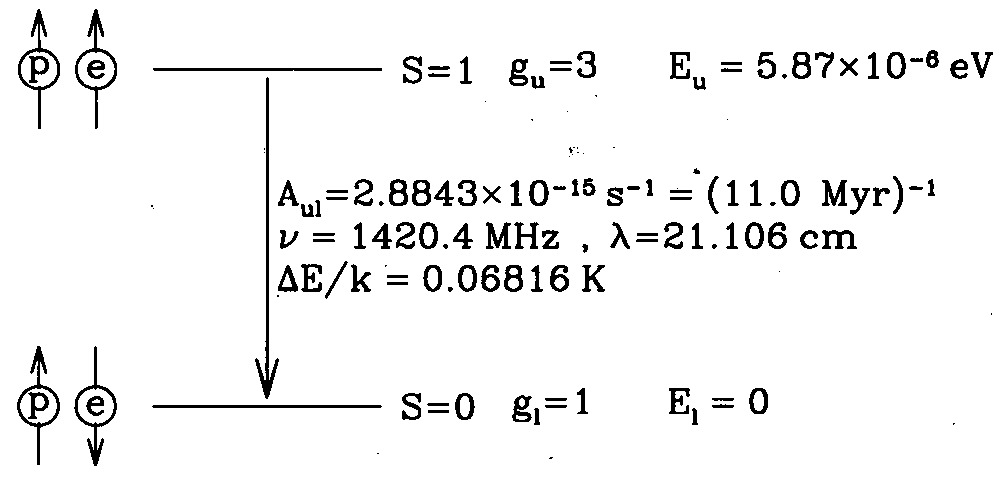
\includegraphics[width=\columnwidth]{ism_figures/Draine_8-1}
\caption{Draine Figure 8.1, depicting the neutral hydrogen 21 cm transition. Note that $S$ represents the hyperfine total angular momentum, not the spin angular momentum. Originally from Gould (1994).}
\label{fig:spin flip}
\end{marginfigure}
\begin{enumerate}
\item collisions with other hydrogen atoms
\item absorption of thermal radiation (note that $T_{CMB} = 2.7$ K is a \textit{floor})
\item Scattering of Ly$\alpha$ photons--it can cause $T_{spin} \rightarrow T_{kin}$.
\end{enumerate}
Typical values of $T_{spin} \sim 100$ K. Because this transition is a magnetic dipole transition, the Einstein coefficient $A_{21} = 3 \times 10^{-15}\rm \, s^{-1}$, giving the excited state a lifetime of $\sim 10^{11}\,$yr.

Because $kT_{spin} \gg h\nu_{21}$, $n_2/n_1 \simeq g_2/g_1 = 3$; e.g., the upper and lower states are equilibrated and don't depend on the spin temperature.

To get a proper line profile in terms of velocity, we note that 
\[\phi(v) = \phi(\nu) \frac{d\nu}{dv} = \phi(\nu) \frac{v_{21}}{c}.\]

Then, the optical depth of the 21 cm line is
\begin{align}
\tau_\nu &= \frac{3c^2 h A_{21}}{32 \pi k_B \nu_{21}^2}\frac{N_H}{T_{spin}} \phi(v) \nonumber\\
&= 0.549 \left (\frac{N_{\HI}}{10^{21}\,\rm cm^{-2}}\right ) \left (\frac{\phi(v)}{\rm [km\,s^{-1}]^{-1}}\right )\frac{100\, \rm K}{T_{spin}}.
\end{align}
where the velocity width matters, helping determine whether the line self-absorbs or is optically thin.


\subsection{The Saha equation}
The \textbf{Saha equation} tells us the population ratios of \textit{ionization} states.\sidenote{Previously, we've used the \textbf{Boltzmann equation} to figure out \textit{excitation} states. To get a full electron census, we'd want to use both in conjunction.}
It depends on the temperature, $T$, and the number density of electrons, $n_e$. Also, we will use the partition function
\begin{equation}
Z^j(T) = \sum_i g_i^j e^{-E_i/kT} = g_0^j n_{tot}^j / n_0^j.
\end{equation}

So the Saha equation is:
\begin{equation}
\frac{n_{\rm tot}^{j+1} n_e}{n_{\rm tot}^j} = \left (\frac{2\pi m_e kT}{h^2}\right )^{3/2} \frac{2 Z^{j+1}(T)}{Z^j(T)} e^{-h \nu_{j+1 \rightarrow j} / kT}.
\end{equation}

\subsection{Pure hydrogen nebula}
Surrounding a single, massive star (OB star), we find a radiation field with $h\nu \geq 13.6$ eV, corresponding to $\lambda < 912\,$\AA. Photons beyond the Lyman limit are called \textbf{Lyman continuum} or \textbf{Lyman leak} photons.

The rate of production\sidenote{We care about the \textit{number} of ionizing photons (not the luminosity) because any photon can only ionize one atom. Excess energy (as counted in the luminosity) does not contribute to further ionizations, but rather becomes kinetic energy to the electron and/or proton.} of these ionizing photons is $Q$, where $[Q] = \rm s^{-1}$:
\begin{equation}\label{eq:ionization photon rate}
Q = \int_{\nu_{*}}^\infty d\nu\, \frac{L_\nu}{h\nu},
\end{equation}
and where $\nu_* = c / (912\, \textrm{\AA})$, the ionization energy.

Now, we can define the cross-section for ionization as a function of frequency,
\begin{equation}
a_\nu(\nu) = 6.3 \times 10^{-18} {\rm\, cm^2} \left (\frac{\nu_*}{\nu}\right )^4 \frac{\exp[4 -(4/\epsilon)\arctan \epsilon]}{1 - \exp(-2\pi/\epsilon))},
\end{equation}
where $\epsilon \equiv \sqrt{\nu / \nu_* - 1}$ for convenience. Note that $a_\nu \propto \nu^{-3}$. Then, the rate of ionization per unit volume equals the local rate of recombination per unit volume when
\begin{equation}
\label{eq:ionization equilibrium}
n_{\HI}\int_{\nu_*}^\infty d\nu\, \frac{4\pi J_\nu}{h \nu} a_\nu(\nu) = n_e n_p \alpha(T),
\end{equation}
where $\alpha(T)$ is the recombination coefficient. This equation assumes ionization equilibrium.

\HII{} regions can be \textbf{density-bounded}, where ionizing photons escape due to low \HI{} gas density. They can also be \textbf{ionization-bounded}, where the edge of the \HII{} region is defined by the extent beyond which no ionizing photons can reach. We can further define $\alpha_B(T)$, the rate of recombination into \textit{all states} other than the ground state. 

If we volume-integrate equation \eqref{eq:ionization equilibrium}, the left-hand side becomes $Q$, as defined by equation \eqref{eq:ionization photon rate}, and the right-hand side becomes $n_{tot}^2 \propto \alpha_B(T) V_{HII} \sim \alpha_B(T) \cdot 4 \pi r_S^3/3$, and where 
\begin{equation}
r_S = \left (\frac{3Q}{4\pi n_{tot}^2 \alpha_B(T)}\right )^{1/3}
\end{equation}
is the \textbf{Str\"omgren radius}.


\section{Wednesday, 16 September}

\subsection{Fiducial \HII{} regions}
To get a sense of fiducial numbers, let's get some numbers for an \HII region surrounding an O5 star:

\begin{tabular}{cc}
Quantity & Value\\
\hline
$T_{eff}$ & $46120$ K\\
$Q$ & $3.39\times 10^{49}\, {\rm s^{-1}}$\\
$n_H$ & $100\rm \, cm^{-3}$\\
$r_S$ & $4.7$ pc
\end{tabular}

Note that in this case, $r_S$ was calculated by using $\alpha_B (T = 10^4\textrm{ K})$. We've also assumed a high ionization fraction $y = n_e/n_H$ and of course $n_e = n_p$. The rate of recombination into $n \geq 2$, $n_en_p \alpha_B = 2.6 \times 10^{-9} \, y^2\,\textrm{s}^{-1}\,\textrm{cm}^{-3}$.

Thus, the volumetric rate of ionization is
\begin{equation}
\frac{n_{\HI}}{4\pi r^2} \int d\nu\, \frac{L_\nu}{h\nu} e^{-\tau_\nu} \simeq \frac{n_{\HI} Q a_\nu}{4\pi r^2} = 1.8 \times 10^{-4} (1-y) \left (\frac{r}{\textrm{pc}}\right )^{-2} {\rm\, s^{-1}\, cm^{-3}}.
\end{equation}


If we set $n_en_p \alpha_B$ equal to the equation above, and input $y=0.9999$ (e.g., where the \HII{} region begins to become very neutral), we get $r=3.8$ pc. Recall that the entire \HII{} region is $4.7$ pc in radius.

The transition from 50\% ionized to neutral happens over a mean free path $\lambda_{\rm MFP}$ of an ionizing photon,
\begin{equation}
\lambda_{\rm MFP} = \frac{1}{0.5 n_H \nu_T} = 10^{-3} \text{\, pc} \ll r_S.
\end{equation}
This mean free path is comparable to the solar system size (whereas the entire ionized region is far larger).

\subsection{Absorption lines}
We primarily study the intergalactic medium via absorption lines illuminated by a background quasar. We begin by using the equation of radiative transfer,
\begin{equation}
I_\nu = I_{\nu, 0} e^{-\tau_\nu} + B_\nu(T_{\rm ex}) \left (1 - e^{-\tau_\nu}\right ),
\end{equation}
where the first term is absorption and the second term is emission at the excitation temperature. In absorption-line systems, we can assume emission to be unimportant (stimulated emission is negligible due to low $T_{\rm ex}$). Then the absorption coefficient, using the oscillator strength $f_{12}$ becomes
\begin{equation}
\alpha_\nu = \frac{h \nu_{21}}{4\pi} n_1 B_{12} \phi(\nu) = \frac{\pi e^2}{m_e c} f_{12} n_1 \phi(\nu),
\end{equation}
so that the optical depth is 
\begin{equation}
\tau_\nu = \int ds \alpha_\nu = \frac{h \nu_{21}}{4\pi} n_1 B_{12} \phi(\nu) = \frac{\pi e^2}{m_e c} f_{12} N_1 \phi(\nu),
\end{equation}
where we have assumed that the number density is constant throughout the path in order to compute the column density $N_1 = \int ds\, n_1$.

We will assume a gaussian line profile,
\begin{align}
\phi_\nu &= \frac{1}{\sqrt{2\pi}} \frac{c}{\sigma_v \nu_0} \exp\left (-\frac{1}{2}\left [\frac{\Delta \nu / \nu_0}{\sigma_v/c} \right ]^2\right ) \nonumber \\
&= \frac{1}{\sqrt{\pi}} \frac{\lambda}{b} \exp\left (- \left [\frac{\Delta v}{b}\right ]^2\right ),
\end{align}
and $b \equiv \sigma_v \sqrt{2}$ is the Doppler parameter. And thus the optical depth is
\begin{equation}
\tau_\nu = \frac{\sqrt{\pi} e^2}{m_e c} \frac{N_1 f_{12} \lambda}{b}\exp\left (-\left [\frac{\Delta v}{b}\right ]^2\right ).
\end{equation}

The optical depth at the \textit{center} of the line profile, $\tau_0$, is
\begin{align}
\tau_0 &= \tau_\nu \exp\left (\left [\frac{\Delta v}{b}\right ]^2\right ) \\
&\approx 0.7580 \left (\frac{N_1}{\rm 10^{13}\, cm^{-2}}\right )\left (\frac{f_{12}}{0.4164}\right ) \left (\frac{\lambda_{12}}{1215.7\, \rm \AA{}}\right )\left (\frac{b}{10\rm\, km\, s^{-1}}\right )^{-1}, \nonumber
\end{align}
and where the fiducial values of the Ly $\alpha$ transition are given.

So how do we measure tiny dips in some continuum at small optical depth? We can define the \textbf{equivalent width} of an absorption line (which is important, because it's \textit{independent of spectrograph resolution}):
\begin{equation}
W_\lambda = \int d\lambda \, \left (1 - \frac{I_\nu}{I_{\nu, 0}}\right ) = \lambda_0 \int \frac{d\nu}{\nu_0}\left (1 - e^{-\tau_\nu}\right ).
\end{equation}
Draine prefers to use the \textbf{dimensionless equivalent width}, $W = W_\lambda / \lambda_0$. 

\subsection{The curve of growth}

\begin{figure}
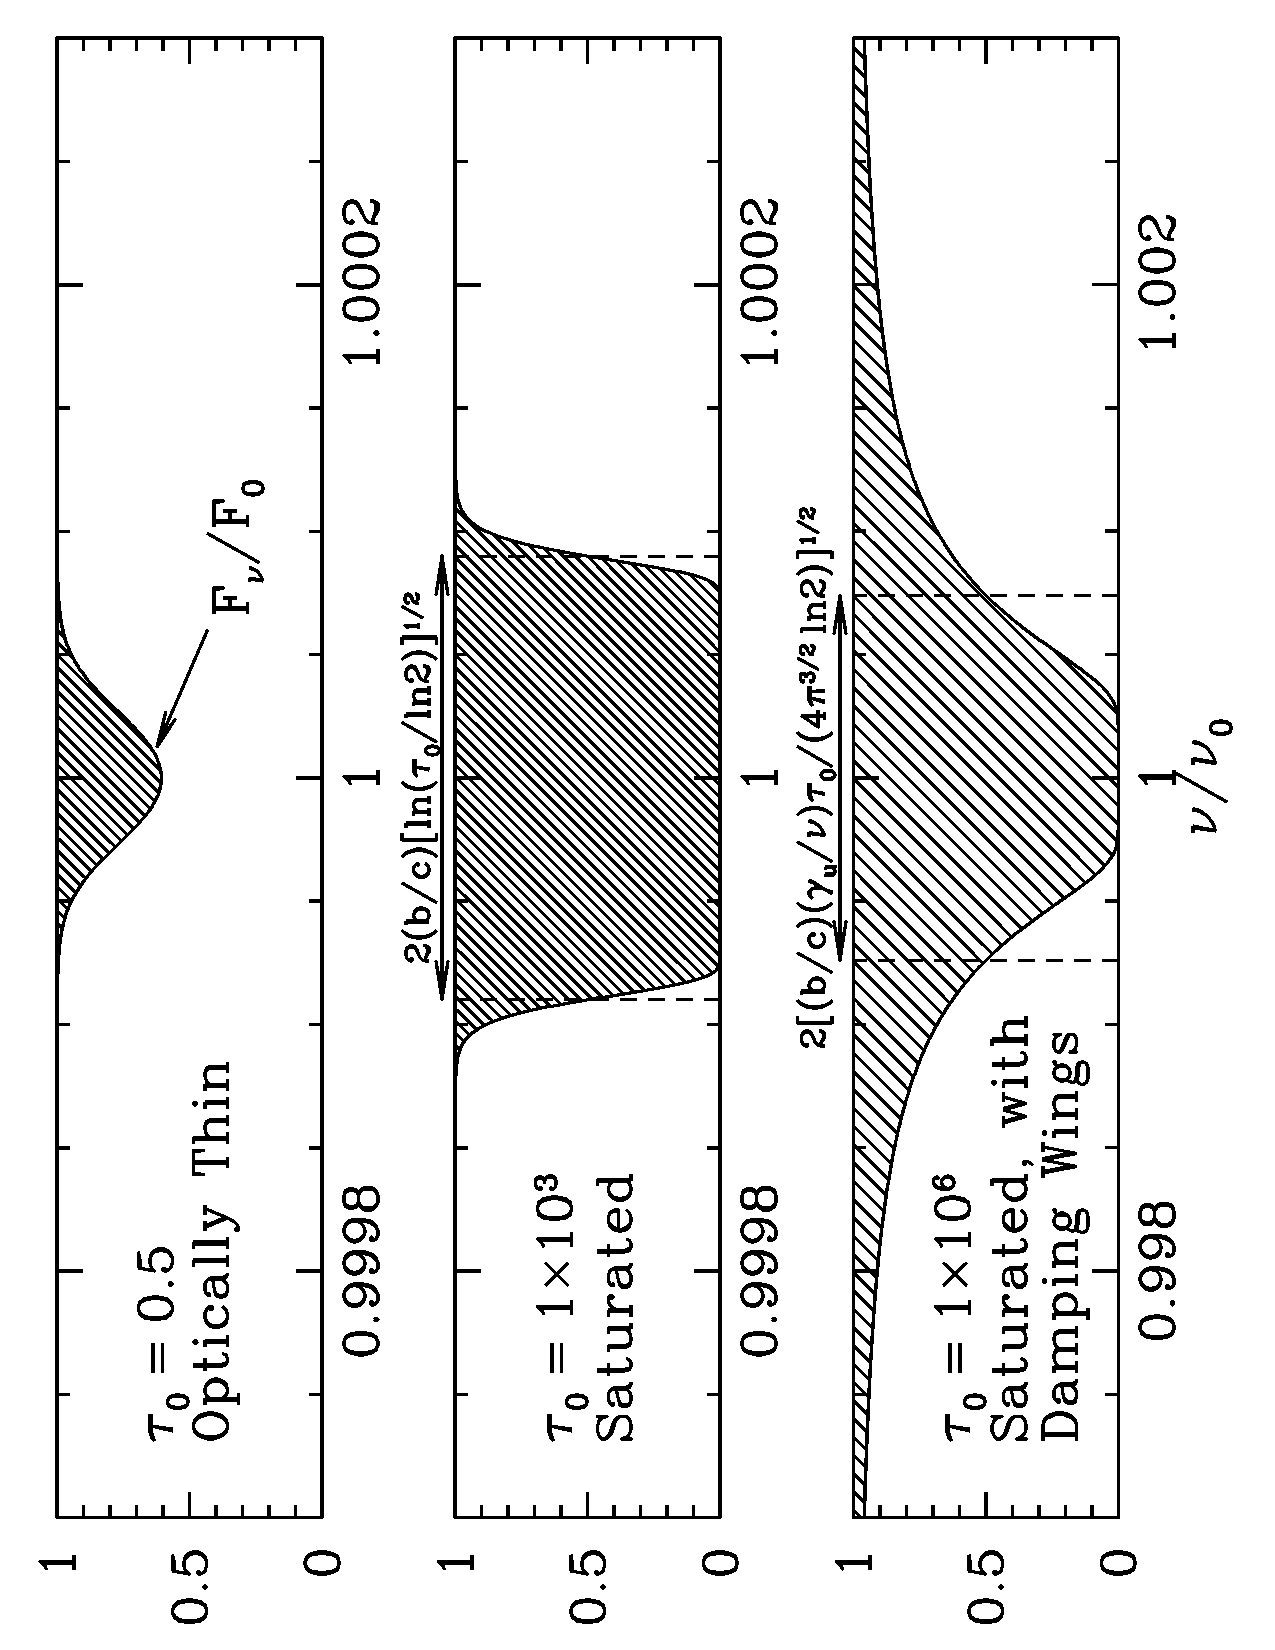
\includegraphics[width=0.8\columnwidth, angle=-90]{ism_figures/Draine-9_1}
\caption{Draine figure 9.1 showing the three regimes of the curve of growth.}
\label{fig:regimes of absorption line systems}
\end{figure}

There are multiple regimes (three that are important) of optical depth, each of which specifically affect $W_\lambda$ dependence on the column density $N_1$:
\begin{enumerate}
\item \textit{Linear regime} ($\tau_0 \leq 1$, so that $1 - e^{-\tau_\nu} \approx \tau_\nu$):
\begin{equation}
W = \int \frac{d\nu}{\nu_0}\tau_\nu = \frac{1}{\nu_0} \frac{\pi e^2}{m_e c} f_{12} N_1 \int d\nu \, \phi(\nu),
\end{equation}
or
\begin{equation}
N_1 = \frac{m_e c^2}{\pi e^2}\frac{1}{f_{12} \lambda} \frac{W_\lambda}{\lambda}.
\end{equation}
\item \textit{Intermediate regime} ($10 \leq \tau_0 \leq 10^3$, so optically thick)
We can approximate this by imagining a square profile between $\tau_\nu =1$ points, so that $W \propto \sqrt{\ln N_1/b}$.

This is called the ``flat'' part of the curve of growth, signifying a weak dependence of $W_\lambda$ on $N_1$.

\item \textit{Saturated regime} ($\tau_0 \geq 10^5$). We can use the ``damping wings'' because the intrinsic broadening dominates over Doppler broadening. If we define the sum over all spontaneous transitions $\gamma_2 = \sum_i A_{2i}$, to get
\begin{equation}
W = \left (\lambda_0 \gamma_2 N_1 f_{12} \lambda \frac{e^2 }{\pi m_e c^3}\right )^{1/2} \propto N_1^{1/2}.
\end{equation}

Therefore, this is the ``square root'' portion of the curve of growth (or damped portion).
\end{enumerate}

\subsection{Spectroscopic notation}
The wavefunction of a single electron is characterized by four quantum numbers
\begin{itemize}
\item $n$: the mean distance from nucleus
\item $\ell$: shape of orbital, eigenvalue of $J^2$, ranges from 0 to $n-1$. 
For example, for $\ell = 0, 1, 2, 3 \rightarrow s, p, d, f$
\item $m$: the eigenvalue of $J_z$, ranges from $-\ell$ to $\ell$
\item $s$: the spin, either $\pm 1/2$
\end{itemize}
E.g., a notation of $n \ell^x$ means that there are $x$ electrons in some orbital ($n, \ell$).

For multiple electrons, we characterized unfilled shells/subshells:
\begin{itemize}
\item $L = \sum_i \ell_i$: orbital angular momentum. We use capital letters, e.g., $0, 1, 2, 3 \rightarrow S, P, D, F$
\item $S = \sum_i s_i$: spin angular momentum, e.g., where $2S+1 = 1, 2, 3, 4 \rightarrow$ singlet, doublet, triplet, quartet
\item $\vec J = \vec L + \vec S$: total angular momentum, which has degeneracy $2 J + 1$.
\end{itemize}
Electron energies depend on $L, S, J$: we split terms given by $L$ and $S$--which then split further by spin-orbit coupling into fine structure levels given by $J$. For a give $L$ and $S$, the number of fine structure levels is $\min (2S+1, L+1)$.

E.g., we label these as $^{2S+1} L_J$.

The ordering of levels follows \textbf{Hund's rules} (for the ground state):
\begin{itemize}
\item higher $S$ leads to lower energies
\item given $S$, higher $L$ leads to lower energy
\item given $L, S$, if outer shell is less than half full, ``normal'' ordering where lower $J$ leads to lower energy. Otherwise it's the other way around
\end{itemize}

Let's now consider the ground state of singly-ionized nitrogen, N\smallcaps{II}. The six electrons are then labeled: $1s^2 2s^2 2p^2$, where the last subshell is unfilled. 

What if we have two electrons? See the table in the equation sheet--showing which states are allowed via the Pauli exclusion principle. We are allowed $S=0$ or $1$, and $L =  0, 1, 2$, so we end up with $^1 S_0, ^1D_2$, and $^3P_0, ^3P_1, ^3P_2$. 

The full level diagram looks like Draine figure 4.1, which is shown in the margin.
\begin{marginfigure}
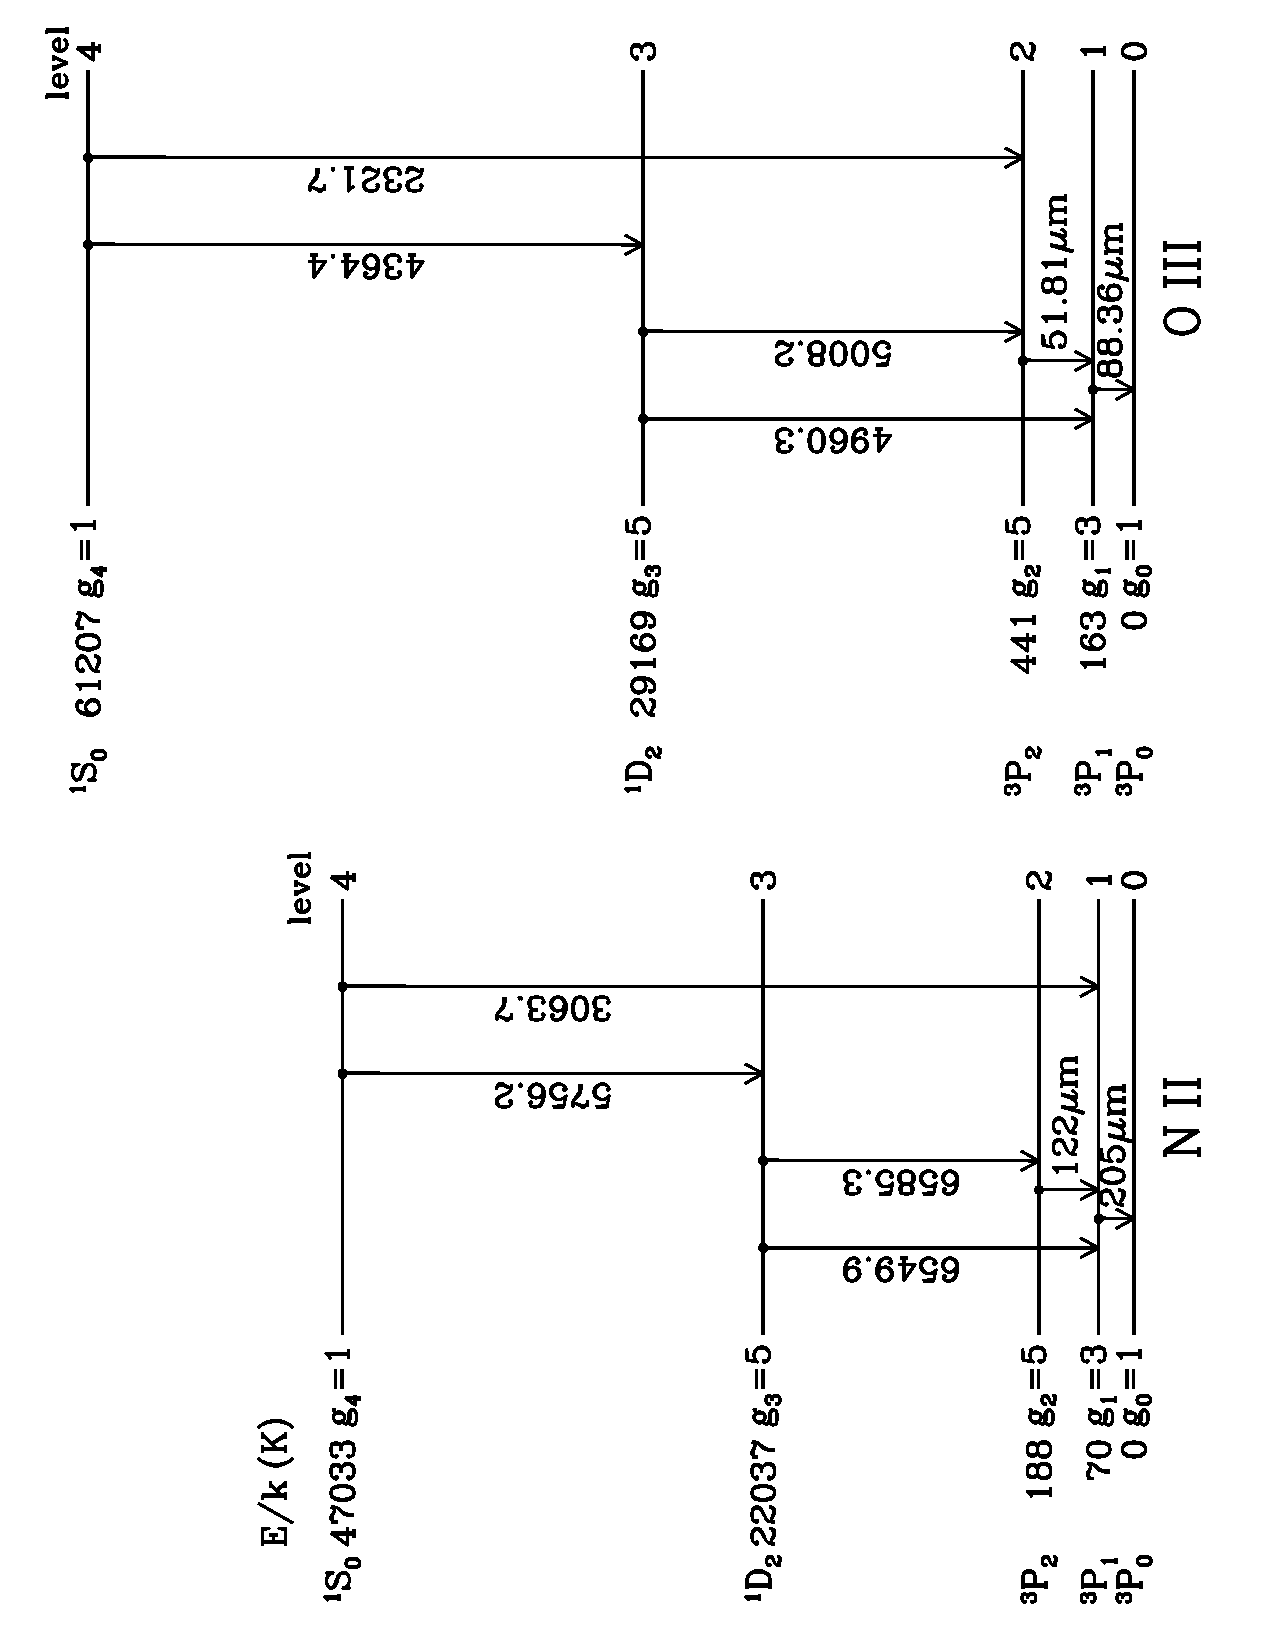
\includegraphics[width=\columnwidth, angle=-90]{ism_figures/Draine-4_1}
\caption{See Draine figure 4.1 showing the electron configurations for N\smallcaps{II} and O\small{III}.}
\label{fig:regimes of absorption line systems}
\end{marginfigure}


\section{Friday, 18 September}
\subsection{Recombination of hydrogen}

A \textbf{recombination cascade} occurs when electrons have more than one recombination/de-excitation states to choose from, e.g., $n=3 \rightarrow n=2$ (H$\alpha$) or $n=3\rightarrow n=1$ (Ly$\beta$).

There are two regimes for recombination:
\begin{itemize}
\item Case A recombination: all photons produced in the recombination cascade escape (an \HII{} region), so that the region is optically thin, or equivalently, density-bounded.
\item Case B recombination (usually more relevant): all non-Lyman series photons escape, but Lyman line and Lyman continuum photons (LyC) \textit{besides Ly$\alpha$} are instantly reabsorbed. The \HII{} region is therefore ionization-bounded, or equivalently optically thick.
\end{itemize}


Remembering our selection rules, and considering hydrogen, we see that Lyman photons must go from $np \rightarrow 1s$. From $3p\rightarrow 1s$, the Ly$\beta$ photon is very easily absorbed when on-resonance by another electron in the $1s$ state (even more easily than LyC photons). Since Case B recombination is far more common in \HII{} regions, the only way for photons to escape is via the cascade, where we get something like $3p \rightarrow 2s \rightarrow 1s$, producing Ly$\alpha$ and H$\beta$ photons that can escape.\sidenote{Note that the $2s \rightarrow 1s$ transition is heavily forbidden, and in high density regions, $2s \rightarrow 2p \rightarrow 1s$ (via collisional excitation and then spontaneous emission, respectively) is more favored.}

A generalization can be made: every Lyman photon with upper level $n \geq 3$ will be converted into either
\begin{itemize}
\item either a Ly$\alpha$ photon or two continuum photons (that sum to Ly$\alpha$ energy)
\item one Balmer series photon
\item sometimes photons from higher series
\end{itemize}

Ly$\alpha$ is resonantly scattered, because $2p \rightarrow 1s$ photons can easily excite another nearby neutral hydrogen. They also might get absorbed by dust. Ly$\alpha$ photons have very long path lengths in the ISM because they are always resonant scattering and random walking through a far greater column density (than, say, LyC photons, which do not resonantly scatter). This is called dust quenching.\sidenote{Actually, this depends on the dust morphology in or near an \HII{} region. Recent literature have shown that Ly$\alpha$ photons do not get significantly more quenched than LyC photons.}

\subsection{Star formation rates}

H$\alpha$ is nice because it will always leave the \HII{} region. Therefore it traces the star formation rate quite well.
\begin{equation}
L_{H\alpha} \propto n_e n_p \alpha_B \Delta V \propto Q.
\end{equation}

The rate of photons emitted from a \textit{cluster} of stars is
\begin{equation}
Q_{\rm cluster} = M_{\rm tot} \int_{m_{L}}^{m_U} dm \int_{\nu_T}^\infty d\nu\, \frac{L_\nu(m)}{h\nu}\Phi(m),
\end{equation}
where $\Phi(m)$ is the initial mass function (IMF), which determines the mass distribution of stars as they are formed. Kennicutt (1998) reviews SFR estimation techniques.

\subsection{Collisional transitions and critical density}
Let's assume a two (or more) level set of energy states, with $E_2 = E_1 + h\nu_{21}$. The relative populations can be affected by absorption and emission, as well as collisions with dominant ``collider'' species (electrons, H, H$_2$) that may impart $\Delta E>h\nu_{21}$ and excite the state (\textbf{collisional excitation}), or steal away exactly $h\nu_{21}$ (\textbf{collisional de-excitation}).

In order for collisional excitation, the collider must have a minimum kinetic energy $mv_{\rm min}^2 / 2 \geq h\nu_{21}$. We can represent these as cross sections, where
\begin{equation}
\gamma_{12}= \left \langle \sigma_{12}v\right \rangle = \int_{v_{\rm min}}^\infty dv\, \sigma_{12} f(v),
\end{equation}
where $[\gamma_{12}] = [{\rm cm^3\, s^{-1}}]$. However, to get a volumetric rate of collisions, we'd want $n_{\rm collider}n_1\gamma_{12}$. For de-excitations, we'd imagine $v_{\rm min} =0$ and simply reverse the subscripts $1 \leftrightarrow 2$.

For a velocity distribution $f(v)$, we often will assume \textbf{Local Thermodynamic Equilibrium}, or LTE. In this case $T_{\rm kin}$ is well-defined and our velocity distribution is a Maxwellian distribution (properly normalized):
\begin{equation}
f(v) =\left (\frac{m_{\rm collider}}{2\pi k T_{\rm kin}}\right )^{3/2} v^2 \exp\left [-\frac{m_{\rm collider} v^2}{2 k T_{\rm kin}}\right ].
\end{equation}
Averaging $\sigma v$ over a Maxwellian leads to the simple relation $\langle \sigma v \rangle \propto T_{\rm kin}^{-1/2}$.

In LTE, our excitation and de-excitations are equal ($n_{\rm collider} n_1 \gamma_{12} = n_{\rm collider}n_2 \gamma_{21}$), leading to our well-known 
\[\frac{\gamma_{12}}{\gamma_{21}} = \frac{n_2}{n_1} = \frac{g_2}{g_1}\exp\left (- \frac{h\nu_{21}}{kT_{\rm kin}}\right ),\]
which makes sense, because $T_{\rm kin}$ acts in the same way as a thermal bath of photons (even though we're imagining a bunch of colliding particles). This is true in LTE without radiative transitions (that we never accounted for). However, these derived relationships for collisional transition coefficients are true \textit{even when radiative transitions are included}--so long as we're in LTE.

What if we assume non-LTE with both collisional and radiative transitions important? Then, we combine their terms\sidenote{I'm abbreviating $n_{\rm collider} = n_{\rm coll}$}
\begin{equation}
n_1\left (n_{\rm coll}\gamma_{12} + B_{12}\bar J\right ) = n_2 \left (n_{\rm coll} \gamma_{21} + B_{21}\bar J + A_{21}\right ),
\end{equation}
and still substitute the $B$ coefficients with previously-derived definitions:
\begin{equation}
\frac{n_2}{n_1} = \frac{n_{\rm coll} \gamma_{12} + (g_2/g_1)(c^2 / 2h\nu_{21}^3) A_{21} \bar J}{n_{\rm coll} \gamma_{21} + (c^2 / 2h\nu_{21}^3) A_{21}\bar J + A_{21}}.
\end{equation}

For now, if we assume $\bar J \rightarrow 0$, then, using a \textbf{critical density} $n_{\rm crit} \equiv A_{21} / \gamma_{21}$:
\begin{equation}
\frac{n_2}{n_1} \rightarrow \frac{\gamma_{12}/\gamma_{21}}{1 + (n_{\rm crit}/n_{\rm coll})}.
\end{equation}

Thus, we now find that
\begin{equation}
\frac{n_2}{n_1} \rightarrow \frac{g_2}{g_1}\frac{e^{-h\nu_{21} / kT_{\rm kin}}}{1+ (n_{\rm crit} / n_{\rm coll})}.
\end{equation}

In the \textit{high-density} regime, where $n_{\rm coll}\gg n_{\rm crit}$, we get
\[\frac{n_2}{n_1} \rightarrow \frac{g_2}{g_1}\exp\left (-\frac{h\nu_{21}}{kT_{\rm kin}}\right ),\]
signifying that the excitation temperature is equal to the kinetic temperature ($T_{\rm exc} = T_{\rm kin}$). In the high-density regime,
\[n_2 n_{\rm coll}\gamma_{21} \gg n_2 A_{21}.\]

In the \textit{low-density} regime, where $n_{\rm coll} \ll n_{\rm crit}$, then
\[\frac{T_{\rm exc}-T_{\rm kin}}{T_{\rm exc}T_{\rm kin}} = \frac{k}{h\nu_{21}}\ln\left (\frac{n_{\rm coll}}{n_{\rm crit}}\right ) < 0,\]
so that $T_{\rm exc} < T_{\rm kin}$, i.e., the excitations are \textit{sub-thermal}. The collisions can't thermalize our population levels

Let's now drop our assumption, so $\bar J \neq 0$. We'll still have to make some other assumptions, namely that photons produced locally can only be absorbed locally (e.g., this can happen with some velocity gradient in the ISM). We will define the \textbf{escape probability}, $\beta(\tau_{\nu_{21}})$, that a photon formed at an optical depth $\tau_{\nu_{21}}$ from the ``surface'' manages to escape:\sidenote{See Lecture 6 notes equations (21-24) for derivation. Note that we've approximated $\phi(v) = (c/v)\phi(v) \approx c\Delta v / v$.}
\begin{equation}
\tau_{\nu_{21}} = \frac{c^3}{8\pi h\nu_{21}^3} A_{21} n_2 \left (\frac{n_1g_2}{n_2g_1} - 1\right )\frac{\Delta s}{\Delta v}.
\end{equation}
This previous result is referred to as the ``large velocity gradient'' formalism for optically thick radiative transfer.

So, revisiting our previous equations, where we've set the number of photons absorbed equal to the number that haven't escaped, we will define a new $n_{\rm crit}' = \beta(\tau_{\nu_{21}})A_{21}/ \gamma_{21}$, and find
\begin{equation}
\frac{n_2}{n_1} \rightarrow \frac{g_2}{g_1}\frac{e^{-h\nu_{21} / kT_{\rm kin}}}{1+ (n_{\rm crit'} / n_{\rm coll})}.
\end{equation}
Here, \textbf{radiative trapping} absorptions help colliders maintain thermal equilibrium (against spontaneous emission), and reduces the effective critical density.
See Draine chapter 19 for values of escape probabilities, $\beta(\tau_{\nu})$.


\section{Tuesday, 22 September}
% Note:  read Draine 14.2, 27. For the PS3, read chapter 15.2, 37.2

\subsection{The [\spec{C}{II}] fine structure line}
Note that all fine structure lines, e.g., where the spin orbit coupling effect causes $\Delta L$ and $\Delta S = 0$. However, fine structure transitions don't change parity, and neither does a single electron wavefunction ($n\ell$) change.

The [\spec{C}{II}] fine structure line at $\lambda = 158$ \um is the dominant cooling line for diffuse gas in star-forming galaxies. Draine writes the spectroscopic notation as $^2P_{3/2}^o \rightarrow ^2 P_{1/2}^o$ (the $o$ is for odd parity; and a nothing for even parity) in his Figure 17.3.

\subsection{Line luminosities per unit volume}
Let's start from the equation of statistical balance:
\[n_1\left ( n_{\rm coll}\gamma_{12} + B_{12}\bar J \right ) = n_2 \left (n_{\rm coll}\gamma _{21} + B_{21}\bar J + A_{21}\right )   \]
and multiple by $h \nu_{21}$ to get local rates of energy transfer per unit volume. These terms have taken into account all emission and absorption due to spontaneous, stimulated, and collisional effects.

Then the net line luminosity per unit volume (with units ${\rm erg\, s^{-1}\, cm^{-3}}$) is:\marginnote{Note: in general, $\Lambda$ is a volumetric cooling rate. There is also an analogous volumetric \textit{heating rate}, $\Gamma$. However, some authors use $\Lambda \rightarrow n^2 \Lambda$ and $\Gamma \rightarrow n\Gamma$.}
\begin{equation}
\Lambda_{21} = h\nu_{21}\left (n_2B_{21}\bar J - n_1 B_{12} \bar J + n_2 A_{21}\right ).
\end{equation}
Why did we drop the terms involving collisions? They aren't associated with \textit{cooling}--i.e., there's no radiative energy transfer.

However, not all these photons will leave our \HII{} region; that would depend on the optical depth, $\tau_{\nu_{21}}$ (we define the optical depth equal to zero at the cloud's surface, and increasing with penetration). We will the idea of the \textit{escape probability} defined last time, $\beta(\tau_{\nu_{21}})$ to summarize the complex radiative transfer, now giving us
\begin{equation}
\left (n_1 B_{21} - n_2{B_{21}}\right )\bar J = n_2\left (1 - \beta(\tau_{\nu_{21}})\right )A_{21}.
\end{equation}

Substituting this back into our definition of the net line luminosity per unit volume, we get nice cancelations:
\begin{equation}\label{eq:cooling rate}
\Lambda_{21} = h \nu_{21} \beta(\tau_{\nu_{21}}) n_2 A_{21}.
\end{equation}
This makes sense,\sidenote{We're assuming that absorption dominates over stimulated emission, which is true \textit{except} in the case of an inverted population. In the limit of small optical depth, absorption is negligible, and likewise stimulated emission, so that only $A_{21}$ is important.} because the cooling rate is equal to the rate of emitted photons times the escape fraction.

If we wanted to calculate the emergent luminosity from the entire cloud, we simply integrate: $L_{21} = \int dV\, \Lambda_{21}$, where obviously $\Lambda_{21}$ is dependent on position.

\subsection{Heavier elements in \HII{} regions}
Helium can ionize and form its own region called a \spec{He}{II} region. Because the ionization energy for He ($h\nu \geq 24.6$ eV) is larger than for H, then the \spec{He}{II} region will be smaller (only for the most massive stars--O1 to O3 stars will the \HI{} region be of comparable size). The two regions are actually coupled, though, because He recombination lines can ionize \HI, but we won't go through those calculations.

What about metals? Elements such as O, Ne, N, S, etc. are in low abundance, but have energy levels near the ground state due to fine structure ($\vec L + \vec S$) and term ($L, S$) splitting of multiple electrons. They can easily be populated by collisional excitations. But collisional de-excitation doesn't happen often, so \textit{forbidden lines do the job of cooling--and they can rapidly cool the cloud this way}.\sidenote{In high density environments such as our labs, collisional excitations easily depopulate via collisional de-excitation. But not so in the near-vacuum of space.}

From equation \eqref{eq:cooling rate}, we see that the strength of cooling depends on $n_2$ and $\beta(\tau_{\nu_{21}})$. $n_2$ is governed by electrons (over protons, due to their greater velocities). In a neutral or molecular region, \HI{} or H$_2$ will be the respective dominant colliders. Metal lines are optically thin so $\beta \rightarrow 1$. We can set $\bar J = 0$ because the frequency-averaged local radiation field is negligible for a line. 

Using the level population ratios at \textit{low density}, 
\begin{equation}
\frac{n_2}{n_1} = \frac{g_2}{g_1} \exp\left (- \frac{h\nu_{21}}{kT_{\rm kin}}\right )\frac{n_{\rm coll}}{n_{\rm crit}},
\end{equation}
and we find that (referencing equations 8-10 on the Lecture 7 equation sheet):
\begin{equation}\label{eq:low density cooling}
\Lambda_{21} = h\nu_{21} n_{\rm coll} n_1 \gamma_{12}.
\end{equation}

In a \textbf{low density region}, every excitation will lead to a spontaneous emission. That is why the result does not depend on $A_{21}$!

In the \textbf{high density region}, we can follow Lecture 7 equations (11-14) to find
\begin{align}\label{eq:high density cooling}
\Lambda_{21} &= h\nu_{21} n_{\rm crit} n_1 \gamma_{12} \frac{1}{1+ n_{\rm crit}/ n_{\rm coll}}\\
& =h\nu_{21} n_{\rm coll} n_1 \gamma_{12} \frac{1}{1+ n_{\rm coll}/ n_{\rm crit}}.
\end{align}
Here, $A_{21}$ appears implicitly because it's factored into $n_{\rm crit}$. The point is that this cooling rate will be lower than in the low density regime, because collisional de-excitations are taking up the energy which would otherwise be radiatively cooled (and collisional de-excitation does \textit{not} cause energy to leave the cloud).

For electron collisions, we will define \textbf{collision strengths} $\Omega_{21}$ and $\Omega_{12}$ implicitly via
\begin{equation}
\gamma_{21} = \frac{h^2}{(2\pi m_e)^{3/2} (kT_{\rm kin})^{1/2}} \frac{\Omega_{21}}{g_2}
\end{equation}
\begin{equation}
\gamma_{12} = \frac{h^2}{(2\pi m_e)^{3/2} (kT_{\rm kin})^{1/2}} \frac{\Omega_{21}}{g_1}\exp\left (- \frac{h\nu_{21}}{kT_{\rm kin}}\right ).
\end{equation}

Regarding \textbf{dust extinction}, we use the term to refer to \textit{both} attenuation (absorption of photons) and scattering of photons out of our line-of-sight. To measure the dust content, we assume a foreground dust screen (which a good assumption for the Milky Way). Dust extinction is usually worse at shorter wavelengths.

Generally extinction, $A_\lambda$, is parametrized in \textit{magnitudes} via
\begin{equation}
m_\lambda = -2.5 \log\left (\frac{F_\lambda}{F_{\lambda, 0}}\right ) + A_{\lambda}.
\end{equation}
For AB magnitudes, $m_{\lambda} = 23.9 - 2.5 \log (F_\lambda / {\rm mJy}) + A_\lambda$, where $1 \,  {\rm \m Jy} = 10^{-29} {\rm erg\, cm^{-2}\, s^{-1}\, Hz^{-1}}$.

The \textbf{dust law} is given by
\begin{equation}
k(\lambda) = \frac{A_{\lambda}}{A_B - A_V} \equiv \frac{A_\lambda}{E(B-V)},
\end{equation}
which is in terms of the \textbf{reddening}, $E(B-V) = A_B - A_V$ (because the of the preferential extinguishing of bluer light).

To study via emission lines, we could use H$\alpha$ and H$\beta$, which is called the \textbf{Balmer decrement}:
\begin{equation}
\left [\frac{F_{H\alpha}}{F_{H\beta}}\right ]_{\rm obs} = 2.86 \times 10^{0.4 (A_{H\beta} - A_{H\alpha})},
\end{equation}
which, for case B recombination, $T_{\rm kin } = 10^4$ K, has a value of 2.86. To derive $A_{H\alpha}$ or $E(B-V)$:
\[A_{H \beta} - A_{H\alpha}  = A_{H\alpha}\left (\frac{k(H\beta)}{k(H\alpha)} - 1\right ).\]

Dust in \HII{} regions systematically causes us to systematically underestimate the intrinsic $Q$ value, and hence, SFR.

\section{Friday, 25 September}
\subsection{Measuring kinetic temperatures in \HII{} regions}
Remember that if we're looking to characterize the dust extinction, we must measure two different lines of the same species (same element and ionization state). Those lines should be far apart, so as to be able to generalize a dust slope.
If we want to measure the \textit{temperature} (also useful for characterizing the dust), then we must measure the ratio of nearby lines to avoid dust sensitivity.

One set of options is\sidenote{see Draine Fig 6.1.}
\begin{itemize}
\item[] [\spec{N}{II}] 5755 (\term{1}{D}{2}{} - \term{1}{S}{0}{})
\item[] [\spec{N}{II}] 6548 (\term{3}{P}{1}{} - \term{1}{D}{2}{})
\item[] [\spec{N}{II}] 6583 (\term{3}{P}{2}{} - \term{1}{D}{2}{})
\end{itemize}
These lines are forbidden because parity $\Pi_i (-1)^{\ell_i}$ are unchanged, \textit{and} because no single electron wavefunctions change.

The latter two are considered a \textbf{doublet} because they are close in wavelength, although they aren't necessarily related quantum mechanically. They also straddle the H$\alpha$ line, which is convenient. These lines are collisionally excited by can only be de-excited above the critical density, $\gtrsim 100 {\rm cm}^{-3}$. So we still see the lines.

The cooling rate of the [\spec{N}{II}] 5755 line is given by 
\[\Lambda_{SD} = h\nu_{SD}n_e n_P \gamma_{PS} \frac{A_{SD}}{A_{SD} + A_{SP}},\]
where $n_P$ is the number density of ionized nitrogen in the $^3P$ state.

If we treat the latter as a single line, we can find the cooling rate
\[\Lambda_{DP} = h\nu_{DP} n_e n_P \left (\gamma_{PD} + \gamma_{PD}\frac{A_{SD}}{A_{SD} + A_{SP}}\right ).\]
Intermediate steps (equations 3-5 on the Lecture 8 sheet) lead to the ratio of line intensities:
\begin{equation}
\frac{\Lambda_{5755}}{\Lambda_{6548} + \Lambda_{6583}} = \frac{\Lambda_{SD}}{\Lambda_{DP}} \simeq \frac{\nu_{SD}}{\nu_{DP}} \frac{\gamma_{SP}}{\gamma_{DP}}\frac{g_S}{g_D}\frac{A_{SD}}{A_{SD} + A_{SP}} \exp\left (-\frac{h\nu_{SD}}{kT_{\rm kin}}\right ).
\end{equation}
The final bit of this equation allows us to figure out the kinetic temperature ($\propto e^{-25000\,{\rm K} / T_{\rm kin}}$, so it's sensitive to temperatures \textit{below} 25000 K). Note that the first line is hardly observed outside of our galaxies.

Another option, which is more commonly used, is \spec{O}{III} (which has the same number of electrons and similar transitions to \spec{N}{II})
\begin{itemize}
\item[] [\spec{O}{III}] 4363 (\term{1}{D}{2}{} - \term{1}{S}{0}{})
\item[] [\spec{O}{III}] 4959 (\term{3}{P}{1}{} - \term{1}{D}{2}{})
\item[] [\spec{O}{III}] 5007 (\term{3}{P}{2}{} - \term{1}{D}{2}{})
\end{itemize}
Even the latter two lines here form a (crude) doublet. Energy splittings are similar to  [\spec{N}{II}].

We can derive general solutions (or rather, Osterbrock \& Ferland) that are valid above low-density, i.e., $n_e \gtrsim 10^{5}\, \textrm{cm}^{-3}$. These are given as equations (7-8) on the Lecture 8 equation sheet for [\spec{N}{II}] and [\spec{O}{III}] respectively. Qualitatively, we see that a \textit{high temperature} gives us a smaller line ratio, whereas \textit{lower temperatures} give us a larger line ratio (because fewer electrons will be in the higher energy \term{1}{S}{0}{} state). From these equations, we see that \HII{} region temperatures are $T \approx 7000-14000$ K.

\subsection{Measuring density in \HII{} regions}
In this case, we want transitions with the same \textit{lower} level. A common choice is to use
\begin{itemize}
\item[] [\spec{O}{II}] 3726 (\term{4}{S}{3/2}{} - \term{2}{D}{3/2}{})\\
\item[] [\spec{O}{II}] 3729 (\term{4}{S}{3/2}{} - \term{2}{D}{5/2}{})
\end{itemize}
The degeneracy factors are given in the spectroscopic notation ($g_i = 2J_i + 1$), so in this case, our three states \term{4}{S}{3/2}{}, \term{2}{D}{5/2}{}, and \term{2}{D}{3/2}{} have respective degeneracy factors of $g_1 = 4$, $g_2 = 6$, and $g_3 =4$.


In the \textit{low density limit}, $n_e \ll n_{\rm crit}$, we get a single photon for every collisional excitation. Note that $A_{32} \ll A_{31}$ because the gap is so extremely small between the second and third fine-structure states of \spec{O}{II}.

Similarly to before, we can call equations (9), (10) from the Lecture 8 equation sheet. A \textbf{line ratio} of the two gives
\[\frac{\Lambda_{3729}}{\Lambda_{3726}} = \frac{\gamma_{12}}{\gamma_{13}} = 1.5,\]
which shouldn't be surprising--the energies are so similar, so the line ratio is simply the ratio of degeneracies ($g_2/g_3 = 1.5$).

\begin{marginfigure}
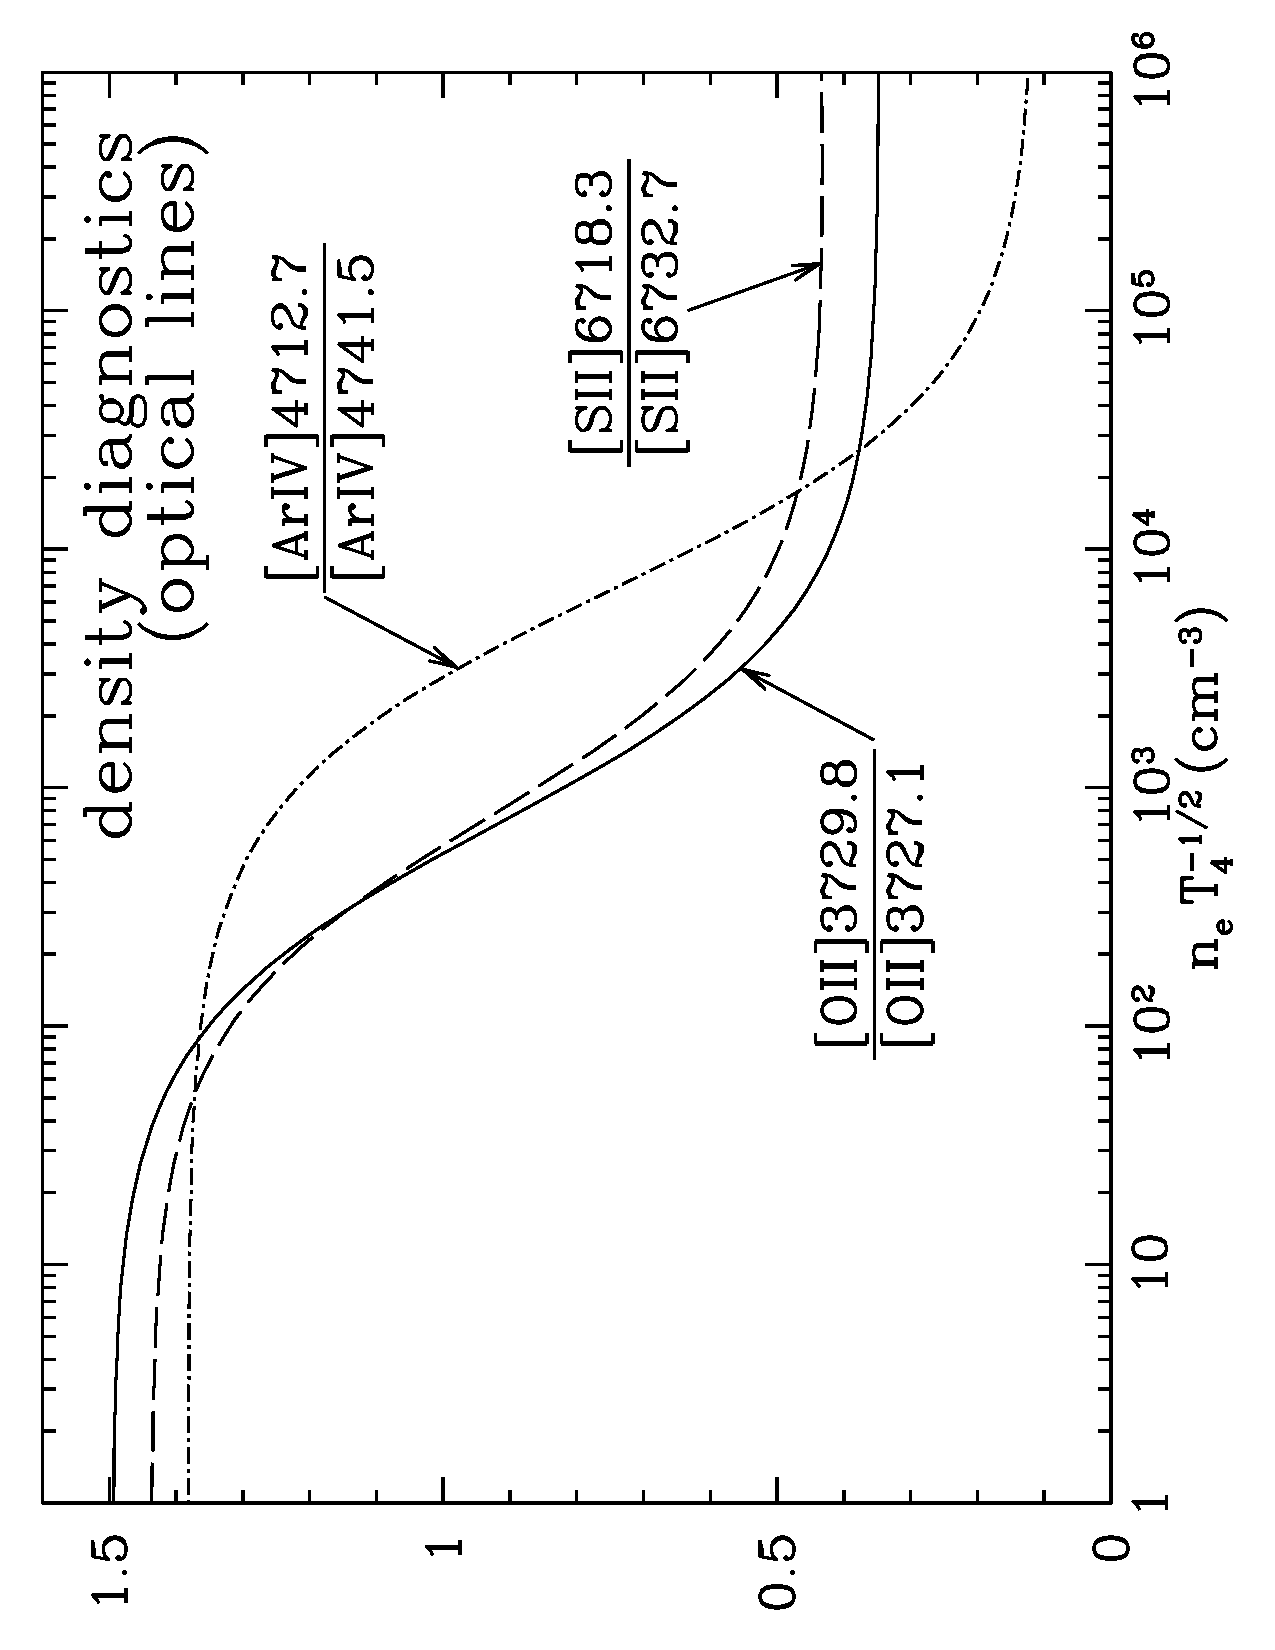
\includegraphics[width=\columnwidth, angle=-90]{ism_figures/Draine-18_4}
\caption{Draine Figure 18.4, showing optical line intensity ratios useful for determining the density.}
\label{fig:determining density}
\end{marginfigure} 
What about in the \textit{high density limit} ($n_e \gg n_{\rm crit}$)? Now things are a little more complicated. Equations (12-16) show all this, culminate in 
\[\frac{\Lambda_{3729}}{\Lambda_{3726}} \simeq \frac{g_2 A_{21}}{g_3 A_{31}} \approx 0.35.\]
The Einstein coefficients are the difference-maker here. This is because our lines are thermalized, and now transitions between the second to third levels may occur far more commonly due to collisions.

See Draine Fig 18.4 in the margin. This diagnostic is sensitive to $n_e (T/10^4 \, \textrm{K})^{-1/2}$ over a range of $10^2 - 10^4\, \textrm{cm}^{-3}$. So we can first measure the temperature (as shown above), and then use it to constrain the density of the gas.

\subsection{Measuring (distant) ionization sources}
Notice the \textbf{BPT Diagram}, shown in Draine Fig 18.7--which allows distinction of AGN from star forming sources.

So why are we using [\spec{O}{III}] 5007 / H$\beta$ 4861 and [\spec{N}{II}] 6583 / H$\alpha$ 6563? The ionization potentials of \spec{N}{I}, \spec{N}{II}, and \spec{O}{II} are 14.5, 29.6, 35.2 eV, respectively. The reason that the BPT star forming component curves to the upper left is because [\spec{N}{II}] decreases and gives way to [\spec{N}{III}] as [\spec{O}{III}] becomes stronger.

\subsection{Measuring metallicity}
Metallicity is usually defined via the relative oxygen to hydrogen abundance ratio. However, ionized oxygen is very common (as we've seen), and we need to sum up \textit{all} ionization states of oxygen to get a proper metallicty. One common method (Pagel et al. 1979) is an empirical indicator:
\begin{equation}
R_{23} = \frac{I_{[\spec{O}{II}] 3727} + I_{[\spec{O}{III}] 4959, 5007}}{I_{H \beta}}.
\end{equation}

Unfortunately, note that [O/H] is actually non-monotonic with $R_{23}$. Metal lines are efficient for cooling (fine structure lines in the far-infrared), which is why at high metallicty, $R_{23}$ decreases. 
Then how do you break this degeneracy? We can use the [\spec{N}{II}] 6583 / H$\alpha$ 6563 line ratio, although this is imperfect too (no [\spec{N}{III}], etc).

The \textbf{ionization parameter} $U$ is
\begin{equation}
U = \frac{Q}{4 \pi r^2 c n_H},
\end{equation}
which is basically $U = n_\gamma / n_H$.\sidenote{Think of $n_\gamma = Qdt/4\pi r^2 dr$.} Empirically, we can use
\[
O_{32} = \frac{I_{[\spec{O}{III}] 4959,5007}}{I_{[\spec{O}{II}] 3727}}
\]
to callibrate $R_{23}$.

\section{Tuesday, 29 September}
% Draine Chapters 27, 30
\subsection{Thermal equilibrium in \HII{} regions}
We kept assuming fiducial values of $T \sim 10^4$ K. How did we derive that?

In the case of thermal equilibrium, heating balances cooling:
\[\Gamma_{\rm tot} = \Lambda_{\rm tot}.\]

The imparted excess kinetic energy from photoionization will be the main heating mechanism. The average extra energy is $\ev{\Delta E} = h\ev{\nu} - h \nu_0$, where $h\nu_0$ is the ionization energy.

Accounting for \textit{all} photons that are around, we find that the heating rate is
\begin{align}
\Gamma_{\rm PI} &= n_e n_p \alpha_A \ev{\Delta E} \nonumber \\
&= n_e n_p \alpha_A(T_{\rm kin}) \frac{\int_{\nu_0}^\infty d\nu \, \frac{4\pi J_\nu}{h\nu} h(\nu-\nu_0) a_\nu }{\int_{\nu_0}^\infty d\nu\, \frac{4\pi J_\nu}{h\nu} \alpha_\nu},
\end{align}\marginnote{Aside: the mean energy decreases as we go further away from the star. This is because the photon-electron cross section \textit{decreases} as we increase in energy above the ionization threshold.}

where we've included the un-normalized distribution of ionization events by averaging $h(\nu-\nu_0)$. Other species behave similarly, but H dominates. Of course, this quantity will depend on the shape of the local ionization spectrum, $J_\nu$ for $\nu > \nu_0$.

The characteristic initial temperature $T_{\rm init}$ of photoionized electrons is 
\[\ev{\Delta E} = \frac{3}{2} k T_{\rm init}.\]
Note that $T_{\rm kin} \neq T_{\rm init}$. However, $\Gamma_{\rm PI}$ depends on $T_{\rm kin}$ via $\alpha_A$ (recombination coefficient), with $\alpha_A \propto T_{\rm kin}^{-1/2}$.

The timescale for an ejected electron to collide with another electron is $\sim 100$ s for $n_e \simeq n_H \sim 100 \, {\rm cm}^{-3}$, and this timescale is inversely proportional to number density. Compare with the timescale for ejected electrons to recombine, $t_{\rm rec} = (\alpha_B n_p)^{-1} \sim 1200$ yr. Because newly ejected electrons collide many times before recombining, the entire \HII{} regions are basically in a \textit{thermal bath} of electrons.

There are three main processes that cool ionized gas:
\begin{enumerate}
\item Recombination

We assume that the initial kinetic energy ($\frac{1}{2}m_e v^2$) of an electron is lost when it recombines with a nucleus. If $\sigma_n(T_{\rm kin})$ is a cross-section for recombination into level $n$, and $f(v)$ is a normalized Maxwellian velocity distribution,
\begin{equation}
\Lambda_{\rm rec} = n_e n_p \sum_{n=1}^\infty \int_0^\infty dv \, v \sigma_n(T_{\rm kin}) \frac{1}{2}m_e v^2 f(v).
\end{equation}

Note also that $\sigma_n \propto v^{-2}$, such that the \textit{slowest} electrons are recombined first. This tends to make $T_{\rm kin} > T_{\rm init}$ (which might seem weird for ``cooling''). The temperature dependence of recombination is $\Lambda_{\rm rec} \propto T_{\rm kin}^{1/4}$.

\item Free-free emission

We've already discussed the power density of free-free radiation,
\[\frac{dW}{d\nu\, dV\, dt} = C_4 n_e^2 T_{\rm kin}^{-1/2} \ln\left (C_3 T_{\rm kin}^{3/2	}/\nu\right ) \exp\left (-\frac{h\nu}{kT_{\rm kin}}\right ).\]
To get a cooling rate, we must integrate over all $\nu$ (and we'll treat the Gaunt factor as approximately constant): $\Lambda_{\rm ff} \propto n_e^2 T_{\rm kin}^{1/2}$.

\item Metal lines

These turn out to be the dominant cooling mechanisms in \HII{} regions and planetary nebulae.
The result from collisional excitation followed by forbidden line radiation.\sidenote{Hydrogen and helium don't operate this way, because their ground states are in the $1s$ orbitals, whereby a $2s$ state requires a relatively large increase in energy. And even when that does happen, the photons can resonantly scatter.} The net effect converts kinetic energy to radiation, which is then \textit{optically thin} in the region.

As we've calculated before,
\begin{align}
\Lambda_{21} &= h\nu_{21} n_2 A_{21} \nonumber \\
&= h\nu_{21} n_e n_1 \gamma_{12} \frac{1}{1+ \left (n_{e}/ n_{\rm crit}\right )}.
\end{align}
\end{enumerate}



So if we assume low $\tau_{\nu_{21}}$ with $\beta(\tau_{\nu_{21}}) \rightarrow 1$, then the total forbidden line cooling rate is the summed cooling rates over all species. It depends on
\begin{itemize}
\item[] the local abundance of a given element
\item[] the distribution of elements' ionization states
\item[] the local density relative to a transition's critical density
\end{itemize}

For an \HII{} region with solar metallicity, $Z_\odot$, $T_{\rm kin} = 10^4$ K, $n_H = 100 \,{\rm cm}^{-3}$, dominant cooling lines are
\begin{itemize}
\item{} [\spec{O}{II}] 3726+3729 $n_{\rm crit} = 3300, 630 {\rm\, cm^{-3}}$
\item{} [\spec{O}{III}] 4959+5007 $n_{\rm crit} = 6.5 \times 10^5 {\rm \, cm^{-3}}$
\item{} [\spec{N}{II}] 6458+6583 $n_{\rm crit} = 7.8 \times 10^4 {\rm\, cm^{-3}}$
\end{itemize}
These are \textit{strongly} sensitive to $T_{\rm kin}$ via $n_2 \propto \exp(-h\nu_{21} / kT_{\rm kin})$.

So far, all cooling and heating rates are proportional to $n^2$, even in the case of species like oxygen, e.g., $n_en_O = n_e^2 (n_O/n_H) \propto n_H^2$. So $T_{\rm equil}$ is \textit{nearly} independent of density. However, the caveat is the $n_{\rm coll}$ vs $n_{\rm crit}$ terms given in the metal line cooling rates. 

\textit{So how do we get to an \HII{} region temperature?} We plot the heating and cooling lines and see at what temperature they balance, i.e., see Draine Fig. 27.1 (top panel). If we change the metal abundances (Draine Fig. 27.2), then of course the metal line cooling (which dominates) will be change, so that the heating-cooling balance will affect the equilibrium temperature. And if we change the densities, $n_H$, we change the collisional de-excitation rates as shown in Draine Fig. 27.3. All of these are of order $T \sim 10^4$ K.

\subsection{Thermal equilibrium in neutral atomic gas}\marginnote{Note that there is some non-zero ionized fraction of hydrogen.}
In a primarily neutral region, there are multiple \textit{heating} mechanisms and only one main cooling mechanism. 

The main coolant is [\spec{C}{II}] (\term{3}{P}{3/2}{o} $\leftarrow$ \term{2}{P}{1/2}{o}) at 158 \um{}. Carbon is the second most abundant element in the ISM, typically one-third is in the gas phase, and the rest is in molecular gas and dust. Most of the atomic hydrogen is C$^+$. The [\spec{C}{II}] splitting of energy levels is $h\nu_{21}/k = 92 $ K.

The dominant collider population in neutral gas is \textit{still} electrons--if and only if we're at low densities, $n_H < 3000 {\rm\, cm^{-3}}$ for typical ionization fraction $y \sim 10^{-3}$. But neutral atoms are the dominant colliders if $n_H$ is higher than that.

The rate of [\spec{C}{II}] colling in low-density limit ($n_{\rm coll} < n_{\rm crit}$) is given by
\begin{equation}
\frac{\Lambda_{[\spec{C}{II}]}}{\rm erg\, cm^{-3}\, s^{-1}} \simeq 3\times 10^{27} \left (\frac{n_H}{\rm cm^{-3}}\right )^{2}\left (\frac{n_C/n_H}{1.4 \times 10^{-4}}\right )\left (1 + 0.42(y/10^{-3})\right ) \exp\left (-\frac{92 \,\rm K}{T_{\rm kin}}\right ).
\end{equation}

Draine Fig. 30.1 shows the cooling rates for different cooling mechanisms, where we see that [\spec{C}{II}] dominates at low temperatures and lower densities.

What about heating? Photons with energy less than $13.6$ eV can ionize elements with low ionization potentials, e.g., C, S, Si (with potentials 11.3, 10.4, 8.2 eV). Most of these will be ionized in the ISM. But this is a \textit{small} source of heating.

Dominant sources of heating will be by
\begin{enumerate}
\item Cosmic rays

We typically talk about highly energetic protons with $1-10$ MeV, and subtracting Ly$\alpha$ radiations, we get a primary energy of $E_{\rm prim} = 7$ eV per ionization. The heating rate is simply
\begin{equation}
\Gamma_{\rm CR} = n_{\HI}E_{\rm prim} \zeta_{\rm CR} \sim 4.6 \times 10^{-27} \left (\frac{n_{\HI}}{\rm cm^{-3}}\right ) {\rm \, erg\, cm^{-3}\, s^{-1}},
\end{equation}
where canonical value of the rate of cosmic ray primary ionizations is $\zeta_{\rm CR} \simeq 3\times 10^{-17}\, {\rm s^{-1}}$.

\item X-rays

Hard X-rays have $E > 250$ eV, and $\zeta_{\rm XR} \simeq 10^{-18} {\rm\, s^{-1}}$. They're not a huge deal but still relevant.

\item Dust

Photoelectric heating of small dust grains (including polycyclic aromatic hydrocarbons, \textbf{PAHs}) dominates the heating mechanism of the neutral atomic gas. The net effect of dust absorptions is the creation of free electrons, which add kinetic energy to the gas.

The \textbf{yield} is the probability that the dust escapes multiplied by the fraction of the photon's energy that is carried off as kinetic energy. For large grains, the yield is about 5\%, but close to 1\% for small grains. For PAHs, the yield is $\sim 15\%$. All this leads to a local heating rate (by the photoelectric effect on dust)
\begin{equation}
\Gamma_{\rm PE} \simeq 5\times 10^{-26} \left (\frac{n_H}{\rm cm^{-3}}\right ) {\rm\, erg\, cm^{-3}\, s^{-1}}.
\end{equation}
\end{enumerate}

The interstellar radiation field, or \textbf{ISRF} is mostly produced by local stars with intensity $G_0$. In the FUV, we measure the intensity using units of \textbf{Habing}: 1 Habing $=1.2 \times 10^{-4} {\rm\, erg\,cm^{-2}\,s^{-1}\,ster^{-1}}$. The local ISRF has $G_0 = 1.7$ Habing.



\section{Friday, 2 October}
% Reference: Chapter 21 
% For next time: read Draine 22-23

\subsection{Neutral atomic gas}

Thermal equilibrium means that heating and cooling are balanced, such that
\[ \frac{\Gamma}{n_H^2} = \frac{\Lambda}{n_H^2}. \]

If we assume the ideal gas law applies, and we know that these rates are functions of temperature, e.g., $\Lambda / n_H^2 = f(T)$, so we can write
\[ \frac{\Gamma}{n_H} \frac{kT}{P} = f(T). \]

Because most heating is due to dust, and dust heating depends on the density of atoms and density of photons, so that $\Gamma / n_H$ is nearly independent of density (and neither is it dependent on temperature).

Now, \textit{assuming a low density limit} (for convenience), we know that we can use \eqref{eq:low density cooling} and find

\[\Lambda_{21} \propto T_{\rm kin}^{-1/2} \exp\left (-\frac{92 {\rm \, K}}{T_{\rm kin}}\right )\]

\begin{marginfigure}
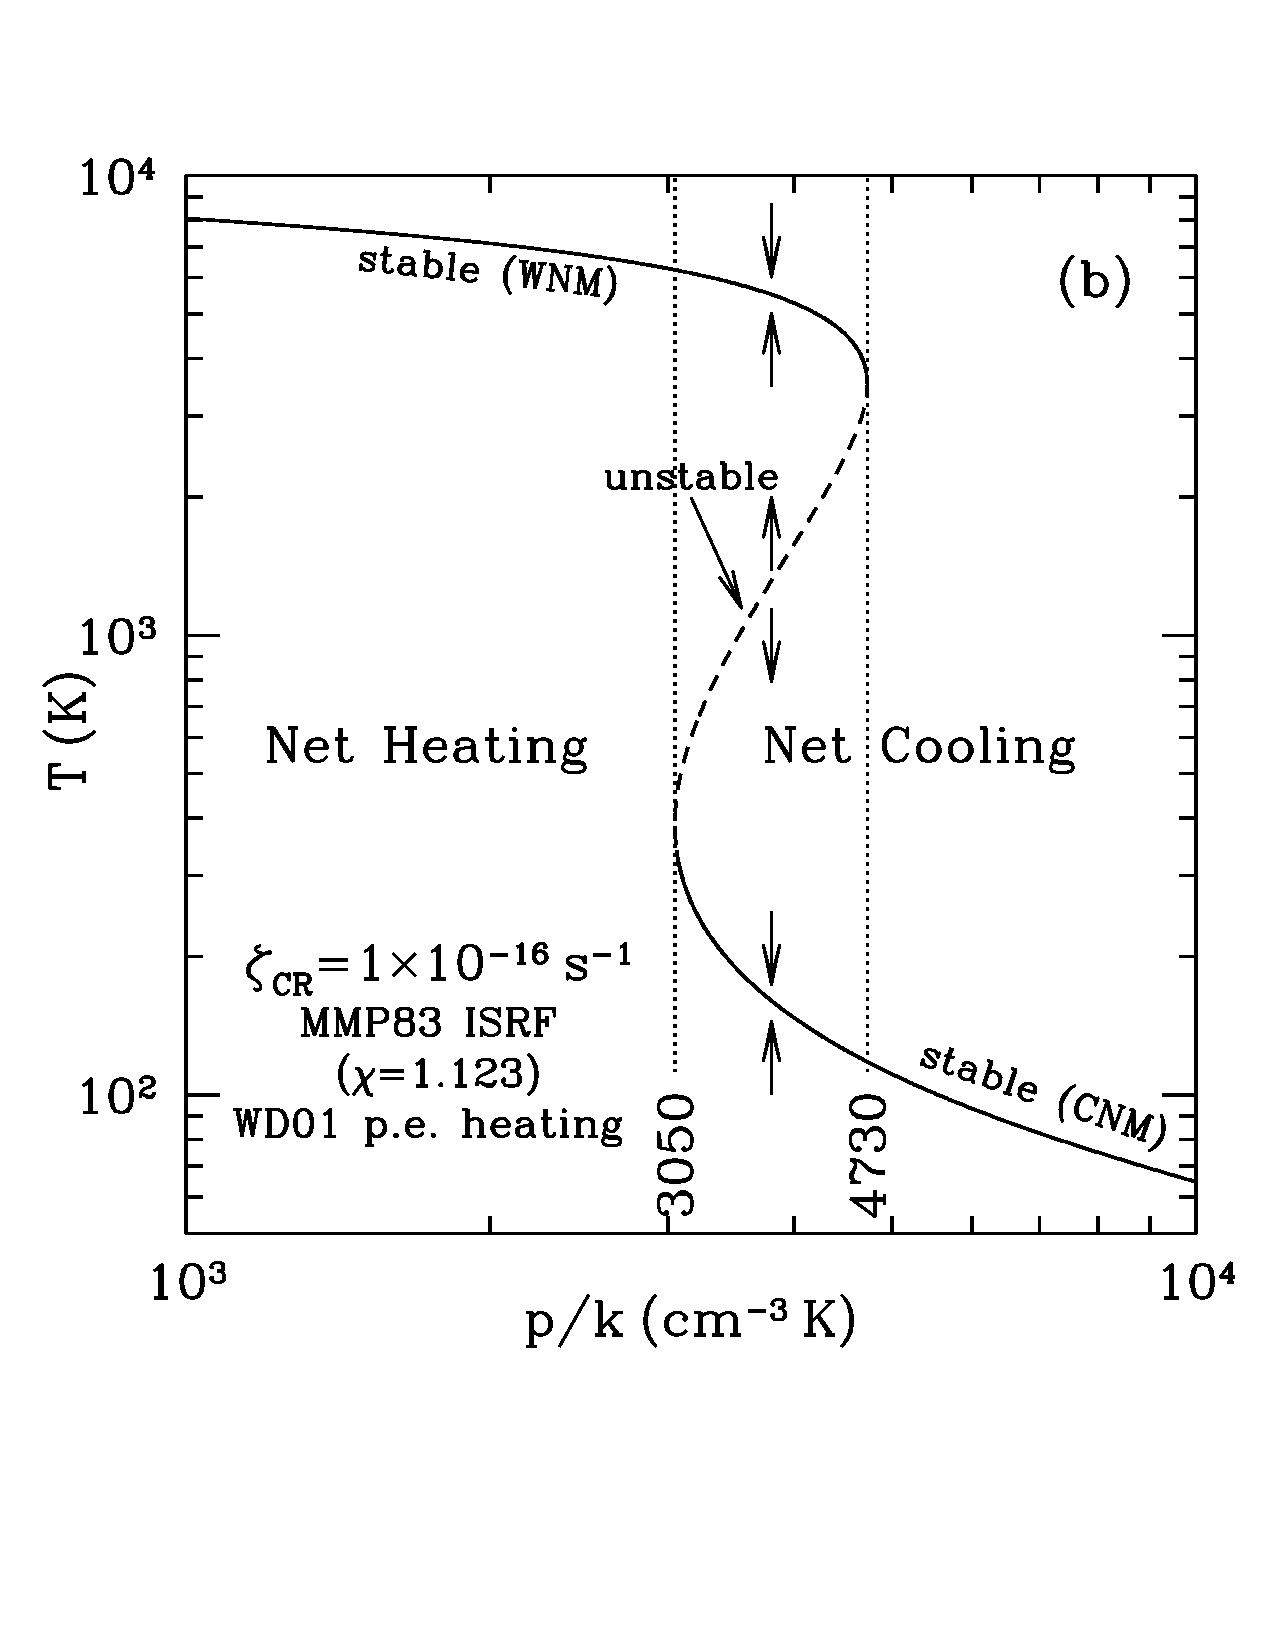
\includegraphics[]{ism_figures/Draine-30_2b}
\end{marginfigure}

We examine Draine figures 30.2 (a) and (b), taking note of panel (b) especially. At the intersection of the cold and warm media, there is \textit{pressure equilibrium} but \textit{not thermal equilibrium} (between $3050$ and $4730 {\rm\, cm^{-3}\, K}$): this \textbf{two-phase ISM} has compressed cold pockets of cold neutral medium (CNM) surrounded by warm neutral medium (WNM). There is also a warm ionized medium (WIM).

This thermal instability is also called an \textbf{isobaric criterion}, and is formally defined as when
\begin{equation}
\frac{\partial (\Lambda - \Gamma)}{\partial T} \bigg\vert_P < 0.
\end{equation}

From above, we can find \[n_H = \left (\frac{\Lambda}{f(T)}\right )^{1/2}.\]

It turns out that we get a two-phase neutral medium IFF $1000 {\rm\, cm^{-3}\, K} \leq P/k \leq 3600 {\rm\, cm^{-3}\, K}$. Or, assuming $P/k = 3000 {\rm\, cm^{-3}\, K}$:


\begin{tabular}{c|ccccccccc}
& $n_H$  & $T_{\rm kin}$ & $y$ & $t_{\rm rec}$   & $t_{\rm therm}$ & $t_{\rm sc}$ & Filling factor & MW scale height\\
& [${\rm cm^{-3}}$] & [K] &  & [yr] & [yr] & [Myr] & & [pc]\\
\hline
CNM & 60 & 50 & $10^{-3}$ & $6\e{4}$ & 3600 & 0.5 & 1\% & 94 &\\
WNM & 0.4 & 7500 & 0.1 & $ \sim6\e{5}$ & $1.6\e{6}$ & 16& 30\% & $\sim 300$ \\
WIM & 0.1 & 8000 &&&&& 25\% & $\sim 900$
\end{tabular}

Some comments:
\begin{itemize}

\item Why is the WNM ionization fraction ($y$) so much higher? It's because the CNM recombination rates are far higher (due to higher $n_H$). 

\item The \textbf{recombination timescale} (of a proton) is given by
\begin{equation}
t_{\rm rec} = \left (\alpha_B n_e\right )^{-1} \sim 200 \left (\frac{T^{0.6}/{\rm\, K}}{n_e/{\rm\, cm^{-3}}}\right ) {\rm\, yr}.
\end{equation}

\item The \textbf{thermal timescale} is the time period for any phase of the ISM to change its energy per unit volume:
\begin{equation}
t_{\rm therm} = \frac{nkT_{\rm kin}}{\Lambda}.
\end{equation}

\item The \textbf{sound crossing time} is
\begin{equation}
t_{\rm sc} \simeq \frac{N_H}{n_H c_s},
\end{equation}

where the sound speed is $c_s \simeq 1.4\e{4} (T_{\rm kin}/{\rm K})^{1/2}$.

\item The WIM cannot have a filling factor of 25\% and still have a scale height of $\sim 900$ pc via stellar winds and SNe alone. They must remain ionized due to OB stars. But OB stars have scale height of 70 pc. This means that there \textit{must} be an appreciable fraction ($\sim 15\%$) of photons escaping \HII{} regions--from \textit{density bounded} \HII{} regions.
\end{itemize}

\subsection{Dust}

What are some observed phenomena of dust?
\begin{itemize}
\item extinction at short wavelength, e.g., dark clouds blocking the disk of the MW--caused by dust grains absorbing light
\item reflection nebulae--dust grains scattering starlight into our line of sight (preserves stellar spectra)
\item reddening of starlight due to differential extinction at different wavelengths
\item polarization of starlight--elongated dust grains align with $B$ fields
\item infrared emission from dense clouds--dust re=emitting absorbed energy
\item \textbf{depletion}--the absence of particular elements (especially Fe, Si, C, Ca, etc.) from the gas phase because they're absorbed onto dust grains
\end{itemize}

To be clear, some of these are degenerate. \textit{Extinction} is actually the sum of \textit{absorption} (a.k.a attenuation) and \textit{scattering}.The old version of radiate transfer was given by
\[dI_\nu = -\alpha_\nu I_\nu\, ds,\]
where $\alpha_\nu$ is the lost specific intensity due to \textit{absorption}. Now, we write
\begin{equation}
dI_\nu = -(\alpha_\nu + \sigma_\nu) I_\nu\, ds,
\end{equation}
where $\sigma_\nu$ is the scattering coefficient. We explicitly keep track of scatterings because we need to conserve photon number!

Previously, we parametrized emission via
\[dI_\nu = j_\nu\, ds,\]
but now we note
\begin{equation}
dI_\nu = (j_\nu + \sigma_\nu J_\nu)\, ds.
\end{equation}

This assumes that scattering is coherent (in frequency, e.g., preserves $\nu$) and isotropic. Of course, the latter is tricky, because the photons change direction compared to before, but it simplifies our problem. Explicitly, this assumption is reflected in the use of the averaged radiation field is $J_\nu = (4\pi)^{-1} \int d\Omega \, I_\nu$.

Now, we \textit{assume emission is thermal} so that $\j_\nu = \alpha_\nu B_\nu(T)$, and combine terms:

\begin{align}
\frac{dI_\nu}{ds} &= -(\alpha_\nu+\sigma_\nu) I_\nu + \alpha_\nu B_\nu(T) + \sigma_\nu J_\nu\nonumber\\
&= -\alpha_\nu (I_\nu - B_\nu) - \sigma_\nu(I_\nu - J_\nu)
\end{align}

So we'll need to define a new version of the source function, $S_\nu'$ (versus the original $S_\nu$), as
\begin{equation}
S_\nu' = \frac{\alpha_\nu B_\nu(T) + \sigma_\nu J_\nu}{\alpha_\nu + \sigma_\nu},
\end{equation}
and
\begin{equation}
\frac{dI_\nu}{ds} = -(\alpha_\nu + \sigma_\nu)(I_\nu - S_\nu').
\end{equation}

So now we can define \textbf{extinction optical depth}, $d\tau_\nu'$,
\begin{equation}
d\tau_\nu' = (\alpha_\nu + \sigma_\nu)\ ds
\end{equation}
so that we get our new equation of radiative transfer
\begin{equation}\label{eq:dusty equation of radiative transfer}
\frac{dI_\nu}{d\tau_\nu'} = - I_\nu + S_\nu'.
\end{equation}

\subsection{Observational perspective of dust}
\marginnote{For a great review of empirical relations of dust extinction, check out Calzetti (2001).}

Let's now assume a foreground dust screen. We can model the extinction
\begin{equation}
F_\lambda = F_\lambda^{\rm no\, dust} e^{-\tau_\lambda'}.
\end{equation}
Be careful with the $F_\lambda$ and $F_\nu$ switches, and don't forget that the primed quantities are \textit{not} derivatives. Our fractional transmission in \textit{magnitudes} are
\[F_\lambda = F_\lambda^{\rm no \, dust} 10^{-0.4 A_\lambda},\] 
\[A_\lambda = -2.5 \log \left (F_\lambda / F_\lambda^{\rm no\, dust}\right ).\]

And it turns out that (because $1 / \ln(2.512) \approx 1.086$),
\[\frac{A_\lambda}{\rm mag} = 1.086 \tau_\lambda'.\]

In a more general case, we might have a distribution of sources mixed with a distribution of dusty clouds. But we'll still assume that the population of sources is uniformly mixed with dust within some slab of thickness $L$. The optical depth through the entire slab is
\begin{equation}
\tau_\lambda' = \int_0^L ds \, (\alpha_\nu + \sigma_\nu).
\end{equation}

Then the observed flux density is
\begin{equation}
F_\lambda = F_\lambda^{\rm no\, dust} \left (\frac{1 - \exp\left (- \tau_\lambda'\right )}{\tau_\lambda'}\right ).
\end{equation}

For example, if $\tau_\lambda ' = 5$ in a \textit{uniformly distributed dust population}, then the fraction of dust-free emission received is 20\% (what's happening here). If $\tau_\lambda' = 5$ for a \textit{complete foreground screen}, we'd received 0.7\% of the emission. However, with the Calzetti law, we usually assume an \textit{effective} foreground screen for simplicity and give us good fits to correct for the dust attenuation.

Our color excess is parametrized by $E(\lambda_1 - \lambda_2) = A_{\lambda_1} - A_{\lambda_2}$: the extra redness is due to the (effective) foreground dust screen of $\lambda_1 - \lambda_2$ color.

We often use $E(B-V)$, where the $B,V$ filters are centered at $\sim 4400$ \AA{} and $5500$ \AA{} respectively. The extinction curve (as we've seen before) is
\begin{equation}
k(\lambda) = \frac{A_\lambda}{E(B-V)},
\end{equation}
and the normalization given by $R_V \equiv k(V) = A_V / E(B-V)$. This is also called the \textbf{total-to-selective extinction ratio}, and it's just a standard. The dust extinction curves are shown in Draine Figures 21.1 and 21.2. Note the 2175 \AA{} ``bump''--which of course is actually an observed trough in our spectra.

Finally, we can apply all this by using the observed Balmer decrement, $F_{H\alpha}/F_{H\beta}$, to calculate the dust law:
\[E(B-V) = \frac{1}{k(H\beta) - k(H\alpha)} \cdot 2.5 \log \left (\frac{F_{H\alpha} / F_{H\beta	}}{2.86}\right )\]

\section{Tuesday, 6 October}

\subsection{Dust extinction (continued)}

The dust column [density] is measured to be higher from hydrogen recombination lines than from UV/optical continuum. This is because the OB stars that ionize hydrogen don't live long enough to drift away from their birth clouds, as opposed to the general UV/optical continuum from potentially older stars. We model this with a simplified geometry of an ``extra'' foreground screen in front of \HII{} regions via
\[E(B-V)_{\rm gas} = \frac{E(B-V)}{0.44}.\]
This factor of $0.44$ is accepted for the local universe but may not be applicable at higher redshift.

The integrated light from a galaxy can also be described by an ``effective'' screen geometry (when dust attenuation is accounted for), e.g., the Calzetti attenuation curve. Star forming regions in the LMC (such as 30 Doradus) do \textit{not} mirror the MW extinction curve (e.g., the 2175 \AA{} bump).

Also in the MW extinction curve, we see \textbf{diffuse interstellar bands} (DIBs; possibly caused by C-C stretching modes). We also see a feature at 3.4 \um due to C-H stretching, and wide 9.7 \um{} Si-O stretching and 18 \um{} O-Si-O bending mode lines. These features can be found in Draine Figures 23.2 and 23.3 (the MW extinction curve is shown in Draine Figure 21.1).

In general, there is a good correlation between color excess and total gas column, implying that the dust-to-gas ratio is nearly constant averaged over large scales. This allows us to write down 
\begin{align*}
\frac{E(B-V)}{\rm mag} &= \frac{N_H + 2N_{H_2}}{5.8\e{21} {\rm\, cm^{-2}}}\\
\frac{A_V}{\rm mag} &= \frac{N_H + 2N_{H_2}}{1.9\e{21} {\rm\, cm^{-2}}},
\end{align*}
where obviously there is the usual factor of 3.1 difference between $A_V$ and $E(B-V)$.

If we look into a dusty region towards a central source, we see further at longer wavelengths. However, this will paradoxically cause us to see a \textit{higher} $E(B-V)$, or dust column, because of the longer optical depth allowed at longer $\lambda$. So we need to measure different wavelength pairs to carefully account for this (e.g., we observe stars near the central super-massive black hole in the MW at NIR wavelengths).


\subsection{Physical properties of dust grains (theoretical)}
We define \textbf{efficiency factors}, $Q$, to be the ratio of the extinction cross section and the effective physical cross section of a dust grain. For dust scattering,
\[Q_{\rm sca}(\lambda) = \frac{\sigma_{\rm sca}(\lambda)}{\pi a^2},\]
where $a \equiv a_{\rm eff} = (3\mathcal V/4\pi)^{1/3}$. For dust absorption,
\[Q_{\rm abs}(\lambda) = \frac{\sigma_{\rm abs}(\lambda)}{\pi a^2}.  \]
This absorption can give rise to thermal emission, so that the \textbf{thermal emission coefficient }is given by
\begin{equation}
j_\nu = n_{\rm dust} Q_{\rm abs}(\lambda) \pi a^2 B_\nu(T_{\rm dust}).
\end{equation}

The total extinction is $Q_{\rm ext}(\lambda) = Q_{\rm sca}(\lambda) + Q_{\rm abs}(\lambda)$, and we can find our total extinction optical depth, including scattering (denoted with primes):
\begin{align}
\tau_\lambda' &= \int_0^L ds \int_{a_{\rm min}}^{a_{\rm max}} da \, n_{\rm dust}(a) \sigma_{\rm ext}(\lambda, a)\\
&\simeq Q_{\rm ext}(\lambda) \pi a^2 N_{\rm dust}.
\end{align}
This result is made only by assuming that the extinction cross section, $\sigma_{\rm ext}$ is independent of position.

The \textbf{albedo} is calculated
\[\tilde w(\lambda) = \sigma_{\rm sca}/ \sigma_{\rm ext} = Q_{\rm sca}/Q_{\rm ext} \leq 1.\] 

In order to calculate cross sections, we need to account for
\begin{itemize}
\item the ratio of $\lambda$ to grain size characterized by $x \equiv 2\pi a / \lambda$ 
\item the grain shapes, because they're generally not spherical
\item the grain composition, which determines electric and magnetic polarizabilities:
\begin{align}
\alpha_E = \frac{p}{E_{\rm app}}\\
\alpha_H = \frac{m}{H_{\rm app}}
\end{align}
based on applied electric and magnetic fields. Recall that $H = B - 4\pi M$, where $M$ is the magnetization within a grain. Furthermore, these depend on their permeabilities $\epsilon$ and $\mu$, which are functions themselves of $\lambda$.
\end{itemize}

To properly solve this crazy last bit, we will need to define a \textbf{complex refractive index} $m = \sqrt \epsilon$ (and $\epsilon$ is now the complex dielectric function; see Draine \textsection 22.2). This leads to \textbf{Mie theory}, as derived by Mie (1908) and Debye (1909). We refer to Draine figures 22.1-22.3, which plot the efficiency factors against $2\pi |m-1| a/\lambda$, which is the phase shift of a wave traveling a distance within grain.

Mie theory is hard stuff, but phenomenologically,
\begin{itemize}
\item for large grains, $Q_{\rm abs} \rightarrow 1$, $Q_{\rm sca} \rightarrow 1$, so $Q_{\rm ext} \rightarrow 2$. Small angle diffractions actually cause this total extinction efficiency to approach \textit{double} the expected absorption (Draine figure 22.3).\sidenote{Even small angles in trajectory along astrophysical path lengths will cause photons to miss their original targets, so this is important in space, but not in a lab.}
\item For intermediate grain sizes, scattering (and hence extinction) $Q$ factors show series of ripples. These ``beats'' are caused by interference between the incident and forward-scattered waves (Draine figure 22.2).
\item The peak efficiency is for grain sizes comparable to $\lambda$. This helps us estimate (crudely) the characteristic dust grain size. It turns out that much of the dust mass is due to dust with $a \approx 0.15$ \um{}. 
\end{itemize}

The \textbf{MRN model} (Mathis, Rumpl, and Nordsieck 1977) is a good, albeit not cutting-edge, model for dust extinction. They proposed power-law distributions of Si and graphite (carbonaceous) grains from 50-2500 \AA{} in size. Those distributions are given by
\begin{align*}
\frac{dn_{\rm sil}}{da} = 7.8\e{-26} \left (\frac{n_H}{\rm cm^{-3}} \right )\left (\frac{a}{\rm cm}\right )^{-3.5}\\
\frac{dn_{\rm gra}}{da} = 6.9\e{-26} \left (\frac{n_H}{\rm cm^{-3}} \right )\left (\frac{a}{\rm cm}\right )^{-3.5}.
\end{align*}

One result of this model is that it assumes two-thirds of all C to be depleted, $\sim 20$\% of all O, and nearly all Mg and F. We do see strong magnesium lines in the NUV, so if this model is correct, then Mg is a terrible predictor of metallicty (and we must be careful using the others). Another implication is that $M_{\rm dust}/M_{H} \simeq 0.01$, suggesting that most of the metals are locked up in dust grains.

The total dust mass (or volume) is then
\[M_{\rm dust} \propto \int da\, a^3 \frac{dn}{da} \propto a_{\rm max}^{0.5} - a_{\rm min}^{0.5},\]
so that the mass (volume) is dominated by the largest grains. The surface area is
\[A_{\rm dust} \propto \int da\, a^2 \frac{dn}{da} \propto a_{\rm max}^{-0.5} - a_{\rm min}^{-0.5},\]
so that the surface area is dominated by the smallest grains. Logically, we also conclude that the number density is dominated by the smallest dust grains.

\subsection{Dust emission}
We'll want to calculate the dust temperature to determine its emission. The volumetric heating rate from the ambient radiation field, $J_\lambda(\lambda)$ is
\[\Gamma_{\rm gr} = 4\pi \sigma_{d} \int_0^\infty d\lambda \, Q_{\rm abs}(\lambda) J_\lambda(\lambda).\]

The emission per volume is then
\[\Lambda_{\rm em} = 4\pi \sigma_d \int_0^\infty d\lambda \, Q_{\rm abs}(\lambda) B_\lambda(T_d).\]

We rewrite the optical depth
\begin{equation}
\tau_\lambda = \int dl \, n_d \pi a^2 Q_{\rm abs}(\lambda),
\end{equation}
where the integral resolves $\tau_\lambda \propto \lambda^{\beta}$. This $\beta$ is the \textbf{emissivity index}, and $\beta \simeq 2$ for metals, $\beta \simeq 1$ for amorphous carbon grains. The observed intensity will be $B_\lambda(T_d)$ modulated by $1 - e^{-\tau_{\lambda}}$, or
\[1-e^{-\tau_\lambda} = 1 - \exp\left [- \left (\frac{\lambda_0}{\lambda}\right )^{\beta}\right ] \simeq \left (\frac{\lambda_0}{\lambda}\right )^{\beta},\]
which also defines the \textbf{emissivity}. Note that $\lambda_0$ is simply the wavelength at which the optical depth is 1.

So then, we can find the expected spectrum in $B_\lambda$ or $B_\nu$:\sidenote{Recall that, despite all of our $\lambda \leftrightarrow \nu$ shenanigans, \[\int d\lambda\, B_\lambda(T_d) = \int d\lambda \, B_\nu(T_d) \frac{c}{\lambda^2}.\]}
\[B_{\lambda}(T_d) (\lambda_0/\lambda)^\beta \propto \lambda^{-5 - \beta}\frac{1}{\exp(hc/\lambda kT_d)-1}\]
\[B_\nu(T_d) (\nu/\nu_0)^\beta \propto \nu^{3+\beta}\frac{1}{\exp{h\nu/kT_d}-1},\]
where now we see the steep \textit{rise} in the spectrum ($3+\beta$), which causes the well-known \textit{positive $k$-correction}.


Nearby bright young stars, we can get $T_d$ via 
\[T_d \simeq 33.5 \left (\frac{a}{0.2 \, \textrm{\um}}\right )^{-0.2} \left (\frac{G_0}{10^4 {\rm \, Habing}}\right )^{0.2} {\rm\, K}\]
in terms of grain size and the ISRF, $G_0$.

Measuring and modelling dust SEDs reveals
\begin{itemize}
\item diagnose whether an obscured source has dust luminosity powered by star formation (SF) or AGN (via $T_d$--warm or hot dust)
\item for AGN, the shape of SEDs can be used to model dust geometry near the black hole (BH)
\item limit to $T_d$: above $T_d \sim 1500$ K, ``sublimation temperature'' would destroy dust grains
\item shape of SED of extragalactic FIR background shows contributions of AGN vs. SF
\item this MRN model fails to explain 2-25 \um{} emission excess caused by transiently heated, small dust grains.
\end{itemize}


\section{Friday, 9 October}
% Read Draine chapters 5, 31 for next time, and Rybicki & Lightman chapter 11

\subsection{Dust grains} % e.g., Draine chapter 25
Dust grains are charged and elongated. Why should dust be charged?
\begin{itemize}
\item Emission of photoelectrons -- volumetric rate $R_{pe} \propto n_e$
\item Accretion of (collisions with) electrons -- volumetric rate $R_{ae} \propto n_e^2$
\item Accretion of (collisions) with positive ions -- volumetric rate $R_{ai} \propto n_e^2$
\end{itemize}
Let's assume for now 2 charge states, $Z_d$ and $Z_d + 1$. Then the fractions $f(Z_d)$ and $f(Z_d + 1)$ are given by
\begin{equation}
f(Z_d) \left [R_{pe}(Z_d) + R_{ai}(Z_d)\right ] = f(Z_d + 1) R_{ae}(Z_d + 1).
\end{equation}
For a multi-charge state, we'd have to balance many terms, etc, similar to our multi-state atom.

In \textit{dense clouds}, $R_{pe}$ is negligible because of the dust shielding. Then the electrons have far higher cross-sections due to their higher velocities, so grains will often have negative charges. This \textit{peak} charge in the charge distribution is like
\[Z_{\rm high\,density}^* \simeq -1.5 \left (\frac{a}{1000 \, {\rm\AA}}\right )\left (\frac{T_{\rm kin}}{100 {\rm\, K}}\right ).\]

In \textit{diffuse clouds}, the photoelectric effect will dominate and our grains should have \textit{positive charge}, with charge distribution peaked at
\[Z_{\rm low\,density}^* \simeq +36 \left (\frac{a}{1000{\rm\, \AA}}\right )\left (\frac{G_0}{1 {\rm\, Habing}}\right ) \left (\frac{T_{\rm kin}}{10^4 {\rm \, K}}\right )^{1/2} \left (\frac{n_e}{0.1 {\rm\, cm^{-3}}}\right )^{-1}. \]

Some general subtleties: Coulomb repulsions/attractions are included, and the Coulomb barrier depends on the charge and size of dust grain. This explains why both of the above scale as $\propto a$ and not $\propto a^2$.

Dust grains are elongated, not spherical. In general, $\vec J$ to align with the principal axis of the largest moment of inertia, $I_1$ \textit{firstly}, and secondly, $\vec J$ will align with any $\vec B$ fields. This leads to polarization of starlight due to differential extinction, given by\sidenote{This is called the Serkowski law, from Serkowski (1973).}
\begin{equation}
p(\lambda) = p_{\rm max} \exp \left (-K \left [\ln (\lambda/\lambda_{\rm max})\right ]^{2}\right )
\end{equation}
Typically, $\lambda_{\rm max} \simeq 5500$ \AA{}, $K \simeq 1$, and we find
\[p_{\rm max} \leq 0.03 \frac{A_{\lambda_{\rm max}}}{\rm mag}.\]

The polarization is less if $\vec B$ is disordered or if it's aligned partially along the line of sight. Also, $\lambda_{\rm max}$ increases with gas density.\sidenote{Because our fiducial polarization peak wavelength is in the optical rather than in the UV, it suggests that large grains with higher absorption tend to either be more spherical, or in regions of disordered $\vec B$ fields.}


\subsection{Molecular energy levels: order of magnitude}
There are three types of energy levels, and we can calculate order-of-magnitude estimates of their energy scales:
\begin{enumerate}
\item Electronic
Given a molecular size $a$, use de Broglie's equation ($\lambda = h/p$) to get $p \sim \hbar / a$:
\begin{equation}
E_{\rm ele} \sim \frac{p^2}{m} \sim \frac{\hbar^2}{m_e a^2},
\end{equation}
where typical $a \sim 10^{-8}$, so we find energy scales of a few eV. Transitions result in \textit{optical/UV wavelength} photons.

\item Vibration 
We will assume a diatomic molecule and treat it like a simple harmonic oscillator, where the potential is $\frac{1}{2}M \omega^2 \xi^2$, where $\xi$ is the displacement from some usual separation, $R_0$, and $M$ is the nuclear mass and $\omega$ the vibrational frequency. Then the electron energy differences are given by
\begin{equation}
\frac{1}{2}M \omega^2 a^2 \sim \frac{\hbar^2}{2 m_e a^2}
\end{equation},
so if $E_{\rm vib} \sim \hbar \omega$, and 
\begin{equation}
E_{\rm vib} \sim \left (\frac{m_e}{M}\right )^{1/2} \frac{\hbar^2}{m_e a^2},
\end{equation}
putting our energy scales $\sim 0.1-0.01$ eV and wavelengths in the infrared (MIR).

\item Rotation

Rotational transitions depend on $J$, with angular momentum $J \hbar$ and 
\begin{equation}
E_{\rm rot} \sim \frac{\hbar^2 J(J+1)}{2I}.
\end{equation}
For a diatomic molecule, $I \simeq \frac{1}{2}Ma^2$ (so long as the two atom masses are comparable), and for small $J$,
\begin{equation}
E_{\rm rot} \sim \left (\frac{m_e}{M}\right )\frac{\hbar^2}{m_e a^2}.
\end{equation}
So rotational energy transitions have $E_{\rm vib} \sim 101^{-3}$ and $\lambda$ is at radio wavelengths.
\end{enumerate}
This allows us to use the Born-Oppenheimer approximation because $E_{\rm ele} \gg E_{\rm vib} \gg E_{\rm rot}$.

\subsection{Electronic bonds}
We will consider $H_2^+$, in which the energetically favorable configuration will look something like $p^+ \cdot e^- \cdot p^+$. We will use the \textbf{Linear Combination of Atomic Orbitals} (LCAO), so that the protons (labeled A and B) can be written in their ground states
\begin{equation}
\psi_A(\vec r) = \frac{1}{\sqrt{\pi a_0^3}} \exp\left (- \frac{|\vec r - \vec R_A|}{a_0}\right ),
\end{equation}
etc. The Bohr radius is $a_0 = 0.529\e{-8}$ cm, and we know that normalized, $\int d^3 \vec r |\psi_{A,B}(\vec r)|^2 = 1$. We can construct molecular states, where $g \rightarrow$ \textit{gerade}, or even, and $u\rightarrow$ \textit{ungerade}, which is odd:
\begin{equation}
\chi_g(\vec r) = C_+ \left (\psi_A(\vec r) + \psi_B(\vec r)\right )
\chi_u(\vec r) = C_- \left (\psi_A(\vec r) - \psi_B(\vec r)\right ).
\end{equation}
Note that 
\begin{equation}
C_{\pm}^{-2} = \int d^3 \vec r \, \left |\psi_A(\vec r) \pm \psi_B (\vec r)\right |^2 = 2 \pm 2\left (1 + \frac{R}{a_0} + \frac{1}{3}\left (\frac{R}{a_0}\right )^2\right )e^{-R/a_0}.
\end{equation}

The Hamiltonian is
\begin{equation}
H = -\frac{\hbar^2}{2_e}\nabla^2 - \frac{e^2}{\vec r - \vec R_A}- \frac{e^2}{\vec r - \vec R_B}- \frac{e^2}{\vec R_A - \vec R_B},
\end{equation}
with expectation value
\begin{equation}
\ev{H_{\pm}} = \int d^3 \vec r\, \chi_{\pm}^*(\vec r) H \chi_{\pm}(\vec r)
\end{equation}
and net binding energy $E_{\pm} - E_{1s}$ given by equation 20 given by the Lecture 20 equation sheet. A negative binding energy is energetically favorable.

Only the \textit{even} state dips negative, resulting in a \textbf{bonding orbital} (dip is to $\sim 2.8$ eV at $R \simeq 1.0$ \AA{}). The odd state remains at positive energy, so that it's an \textbf{anti-bonding orbital}.

Now, for neutral H$_2$, we can build orbitals by combining $\chi_g$ orbitals (adding in Coulomb repulsion of two electrons and watching out for the Pauli exclusion principle). Therefore, we must keep the electron pair at opposite spins, which is the \textbf{singlet anti-symmetric state}:
\begin{equation}
\chi_{\rm singlet} \propto \left (\psi_A(\vec r_1) + \psi_B(\vec r_1)\right )\left (\psi_A(\vec r_2) + \psi (\vec r_2)\right )\phi_{\rm singlet},
\end{equation}

where we can ground cross terms given by ``equations'' (22) and (23) on the Lecture 20 equation sheet. Equation (22) describes an H$^-$ combining with another proton, but that's unlikely; instead we want equation (23), which is the H$_2^+$ scenario. Then the \textit{singlet} and \textit{triplet} states are bound and unbound, respectively, and equations (24-25) on the equation sheet.

\section{Tuesday, 13 October}
\subsection{Electronic states for homonuclear diatomic molecules}
Quantum numbers of relevance include
\begin{itemize}
\item $S$, the total spin
\item $\Lambda$, the orbital angular momentum of electrons \textit{along internuclear axis}
\item $\Omega$, (where $\vec \Omega = \vec S + \vec \Lambda$) the total angular momentum of electrons \textit{along internuclear axis}
\item $u$/$g$, odd/even parity, defined only for homonuclear molecules
\item +/-, reflection symmetry along a plane containing internuclear axis, defined only if $\Lambda = 0$
\end{itemize}
The eigenvalue $\lambda = |m_\ell|$, labeled as $\sigma, \pi, \delta, \phi$ for $\lambda= 0,1,2,3$. Then the total $M_L = \Sigma_i m_{\ell, i}$, and $\Lambda \equiv |M_L|$.\sidenote{But note that $\Lambda \neq \sigma_i |m_{\ell|,i}$.} These $\Lambda$ terms are labeled as $\Sigma, \Pi, \Delta, \Phi$ for $\Lambda = 0, 1, 2, 3$.

If we have spin-orbit coupling, then $\Omega = \Lambda + M_S$, where $M_S$ is the projected spin along the internuclear axis. So the full \textit{term} symbol looks like $^{2S+1} \Lambda_\Omega$.

For H$_2$, the four lowest-energy electronic states are
\begin{itemize}
\item[X] \term{1}{$\Sigma$}{0}{} $g$+ : both electrons are in lowest $\sigma_g\, 1s$ orbital and have opposite spins
\item[b] \term{3}{$\Sigma$}{1}{} $u$+ : ``repulsive'' electrons in $\sigma_g\, 1s$ and $\sigma_u\, 1s$ orbitals with same spins
\item[B] \term{1}{$\Sigma$}{0}{} $u$+ : electrons in $\sigma_g\, 1s$ and $\sigma_u\, 1s$ orbitals with opposite spin
\item[C] \term{1}{$\Pi$}{1}{} $u$ : electrons are in $\sigma_g\, 1s$ and $\pi_u\, 2p$ orbitals with opposite spins
\end{itemize}

\begin{marginfigure}
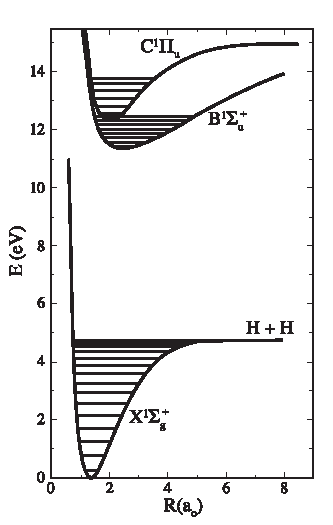
\includegraphics[]{ism_figures/Draine-5_1}
\caption{The energy spectrum of different H$_2$ molecular states (Draine Figure 5.1).}
\end{marginfigure}


See Draine Figure 5.1 (margin) to see some of the electron potentials of the H$_2$ electronic configurations.
Observationally, transitions linking X to B are \textbf{Lyman bands}, and transitions linking X to C are Werner bands--both sets of line transitions are in the rest-UV.


\subsection{Rotational spectra for linear molecules}
In cold, dense environments, we can assume that the molecules are in their lowest electronic and vibrational states, such that only the rotational excitations are allowed.
We diagonalize the moment of inertia tensor to get the principle moments, $I_x, I_y, I_z$.
Typically we see the following molecular shapes:\sidenote{We call them \textit{tops} because they tend to spin}
\begin{itemize}
\item Linear $I_x = I_y$, $I_z \simeq 0$, e.g., CO
\item Oblate (symmetric top) $I_x = I_y < I_z$, e.g., ammonia (NH$_3$).
\item[] Prolate also works, $I_x < I_y = I_z$, e.g., methyl acetylene (CH$_3$CCH)
\item Spherical top $I_x = I_y = I_z$, e.g., methane (CH$_4$)
\item Asymmetric top $I_x \neq I_y \neq I_z$, e.g., formaldehyde (H$_2$CO)
\end{itemize}

Classically, e can write the total energy and angular momentum:\sidenote{Why do we use $J$ as the single quantum number? Only because this tends to behave like a classical system, but it has nothing to do with the total spin-orbit angular momentum of an atom.}
\begin{align}
E &= \frac{\vec J_x^2}{2I_x} + \frac{\vec J_y^2}{2I_y} + \frac{\vec J_z^2}{2I_z}\\
\vec J^2 &= J_x^2 + J_y^2 + J_z^2
\end{align}

The hamiltonian is simply $H_{\rm rot} = J / 2I$, and we find energy levels
\begin{equation}
E_{\rm rot} = \frac{h^2 J(J+1)}{\mu R^2},
\end{equation}
where sometimes we define a \textbf{rotation constant} $B = h/8\pi^2 I$, so that $E_{\rm rot} = h B J(J+1)$.

Selection rules for electronic dipole transitions:
\begin{enumerate}
\item $d \neq 0$. It must have a permanent electric dipole moment, i.e., $d$ cannot equal zero (this is impossible for homonuclear molecules)
\item $\Delta J = \pm 1$
\end{enumerate}

Energy levels can easily be written in terms of frequency $\nu_{J+1 \rightarrow J} = 2B(J+1)$. The quadratically spaced energy levels have linearly spaced energy separations. This is exactly how the CO rotational ladder works.

Remember way back when we derived the $A_{21}$ Einstein coefficient,
\[A_{21} = \frac{64 \pi^4}{3hc^3} \nu_{21}^3 \left |\ev{\psi_1|\vec d | \psi_2}\right |^2.\]

For rotational transition $J+1 \rightarrow J$, 
\[\left |\ev{\psi_{J+1}|\vec d | \psi_J}\right |^2 = d^2 \frac{J+1}{2 J + 3}.\]
All these have assumed a \textbf{rigid rotator}, which ignores centrifugal stretching (a $\sim$ 10\% effect).

The moment of inertia and dipole are affected by \textbf{isotopic composition} because the rotation coefficient $B \propto I^{-1} \propto \mu^{-1}$. So changing the mass leads to

\begin{align*}
\nu &\propto \frac{M_1 + M_2}{M_1 M_2}\\
\frac{d\nu}{dM_1} &\propto -\frac{1}{M_1^2}\\
\frac{\Delta \nu}{\nu} &= -\frac{\Delta M_1}{M_1} \frac{M_2}{M_1 + M_2}
\end{align*}
So, for the case of $^{13}$CO versus $^{12}$CO, we find a shift in frequency
\[\frac{\nu(^{13}CO) - \nu(^{12}CO)}{\nu(^{12}CO)} \simeq -\frac{1}{12} \frac{16}{28} \approx -0.048,\]
again assuming a rigid rotator.

\subsection{Rotational spectra for more complex molecules}
First, we'll examine the energy of a prolate molecule ($I_B = I_B > I_A$):
\begin{equation}
H_{\rm rot} = \frac{J^2}{2I_B} + J_z^2 \left (\frac{1}{2I_A} - \frac{1}{2I_B}\right ).
\end{equation}
This form is nice because the eigenvalues of $J^2$ and $J_z$ are known:
\begin{align}
J^2 \psi &= \hbar^2 J(J+1) \psi\\
J_z \psi &= \hbar K \psi,
\end{align}
where $K \in [-J, -J+1, \ldots, J] $. So, plugging back into the hamiltonian,
\begin{align}
E &= \frac{\hbar^2}{2I_B}J(J+1) + \left (\frac{\hbar^2}{2I_A} - \frac{\hbar^2}{2I_B}\right )K^2\\
&= hBJ(J+1) + h(A-B) K^2,
\end{align}
where $B$ was the old rotational constant and $A$ is a new one. The \textit{oblate} top is exactly the same, except that the constant $A$ is swapped out for another one.

So now we come upon these new selection rules for electric dipole transitions:
\begin{enumerate}
\item $\Delta J = 0, \pm 1$
\item $\Delta K = 0$
\end{enumerate}
The $K$ quantum number \textit{cannot} change via dipole transitions, so, e.g., a molecule starting out with $J=0$ will \textit{always} have $K=0$.


\begin{marginfigure}
\caption{The energy spectrum of ammonia molecules (Draine Figure 5.5).}
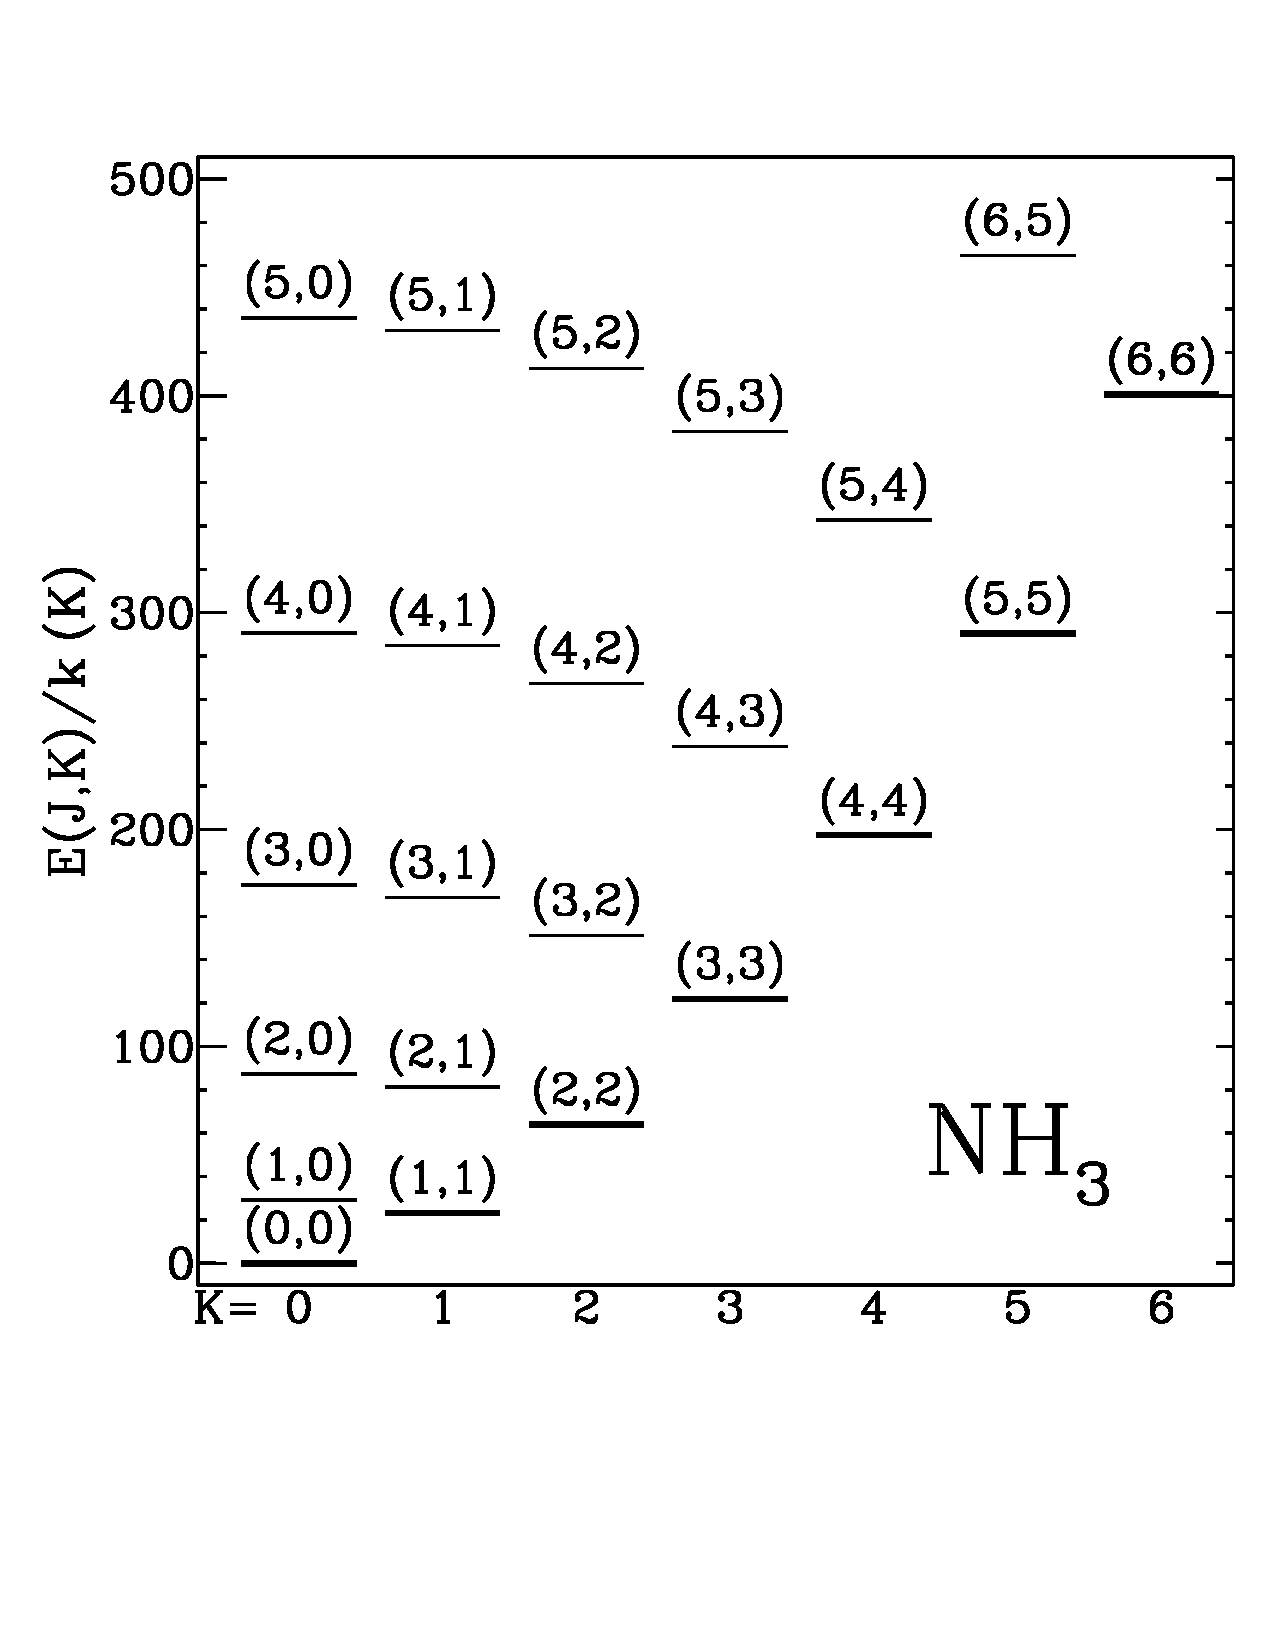
\includegraphics[]{ism_figures/Draine-5_4}
\end{marginfigure}

Draine Figure 5.4 shows the spectrum of NH$_3$, which is an oblate spheroid. The nitrogen can tunnel through the three hydrogen molecules, causing a parity difference and a $\sim 23$ GHz transition.

Finally, nuclear wavefunctions can also break degeneracies in energy splittings. They are called \textit{ortho-} when they are symmetric, and \textit{para-} when anti-symmetric. For water (Draine Figure 5.5) or formaldehyde, we can observe the difference in line populations. The conversion between ortho and para takes $\sim$ a million years. \marginnote{Observing formaldehyde, we can probe its formation history (by default, we'd see a ratio of 3:1 for ortho:para).}


\section{Friday, 16 October}
% Read Draine chapter 32,33 

\subsection{Vibrational spectra}
For a diatomic molecule, we can use a \textit{Morse potential}:
\begin{equation}
U(r) = U_0 + B_n \left [1 - e^{-\beta_n (r-r_0)}\right ]^2.
\end{equation}
These constants, $B_n, \beta_n, r_0$ are fit to each particular molecule (and $n$ refers to the electronic state--impacting the separation of the atomic nuclei). Energy eigenvalues are given by
\begin{equation}
E_{nv} = \hbar \omega_{n0}\left (v + \frac{1}{2}\right ) - \frac{\hbar \omega_{n0}^2}{4 B_n}\left (v + \frac{1}{2}\right )^2,
\end{equation}
where $\omega_{n0} = \beta_n \sqrt{2B_n/\mu}$ and $\mu$ the reduced mass. Note that we get a vibrational quantum number $v$, which is an integer within:\sidenote{The upper energy limit is $E=B_n$, which will basicaly lead to the unbinding of the molecule.}
\[0 \leq v \leq \frac{\sqrt{2\mu B_n}}{\beta_n \hbar} - \frac{1}{2}.\]

A slight digression: Suppose we have a molecule with $N$ atoms--then the number of degreens of freedom, $\mathfrak D$, is $3N$ (in configuration space). We ``lose'' 3 to center of mass translations, 2 or 3 or more to rotations (if linear, etc), leaving $\mathfrak D = 3N-5$ vibrational degrees of freedom if linear (or $\mathfrak D = 3N-6$ or fewer for more general molecules).

Selection rules for electric dipole vibration-rotation transitions of diatomic molecule:
\begin{enumerate}
\item $d \neq 0$ (from before--we require a permanent dipole)
\item $\Delta d |_{r=r_0} \neq 0$, i.e., the dipole moment must change during a change in vibrational state
\item $\Delta v = \pm 1$
\item $\Delta J = \pm 1$ if $\Lambda=0$, or $\Delta J = \pm 1, 0$ if $\Lambda \neq 0$ (for rotations). For pairs of vibrational levels with $v_2 > v_1$, $\Delta J = J_{v_1} - J_{v_2}$
\end{enumerate}
The notation for the $\Delta J = \{+1, 0, -1\}$ transitions are known as the \{P, Q, R\} branches. It is expressed as $v_2 - v_1 \{\textrm{P.Q,R}\}(J_{v_1})$. For example, for CO:
\begin{itemize}
\item[] 1-0 R(0) at 4.657 \um{} links $(v_2, J_{v_2}) = (1,1)$ to $(v_1,J_{v_1})=(0,0)$
\item[] 2-1 P(10) at 4.814 \um{} links $(v_2, J_{v_2}) = (2,9)$ to $(v_1, J_{v_1}) = (1,10)$
\end{itemize}

H$_2$ with $d=0$ can undergo \textit{electric quadrupole} transitions with selection rule
\begin{enumerate}
\item $\Delta J = \{+2, 0, -2\}$ called \{O, Q, S\} branches.
\item No rules on $\Delta v$
\end{enumerate}
We observe strong transitions in the NIR, e.g., 1-0 S(1) at 2.12 \um{} and 2-1 S(1) at 2.25 \um. Can be seen in shocks or near young stars as UV photons excite molecules electronically, but as they hit the electronic ground state in some arbitrary ro-vibrational\sidenote{or vibro-rotational} state, they cascade down the ro-vibrational ladder. In molecular clouds, the lack of collisional excitations prevent these H$_2$ transitions from occurring often.

The statistical weights for $(v,J)$ ro-vibrational levels of H$_2$ are 
\[g_{(v,J)} = g_{o/p}(2J+1),\]
where $g_{o/p} = 3$ for odd $J$ (ortho-H$_2$) and $g_{o/p} = 1$ for even $J$ (para-H$_2$).

\subsection{Electronic-vibrational-rotational transitions}
The full energy level is given by
\begin{equation}
E_{nvJ} = V_{n0} + \gamma_n \hbar^2 \Lambda^2 + \alpha_n \hbar J(J+1) + \left (v+\frac{1}{2}\right ) \hbar \omega_n.
\end{equation}
We have the following selection rules:
\begin{enumerate}
\item $\Delta \Lambda = \{0, \pm 1\}$
\item $\Delta J = \{0, \pm 1\}$ but $J = 0\rightarrow 0$ excluded, and $\Delta J=0$ if $\Lambda = 0\rightarrow 0$
\item $\Delta v =$ \{any non-zero integer\}
\end{enumerate}
See Rybicki \& Lightman Figures 11.7 and 11.8 for PQR branches of these electro-vibro-rotational transitions.

A decay of H$_2$ down to $v>14$ (or $J>5$ for $v=14$) in the ground electronic state, the molecule will unbind. It's not fully intuitive, but the potential for a molecule will change depending on its electronic state.

\subsection{Formation of H$_2$}
There are gas-phase interactions and grain surface interactions to forming moleuclar hydrogen. First we'll examine the gas-phase interaction (more accurately than when we used the LCAO method). 

Can H$_2$ form via radiative association (i.e., H + H $\rightarrow$ H$_2$ + $\gamma$)? Nope, because there's only one photon emitted via a permanent dipole, but $d=0$ for H$_2$.

The best gas-phase formation channel involves
\begin{equation*}
\textrm{H + }e \rightarrow {\rm H^{-}}+ \gamma \Longrightarrow 
\begin{cases}
\textrm{H}^{-} + \gamma \rightarrow \textrm{H} + e\\
\textrm{H}^{-} + H \rightarrow \textrm{H}_2 + e
\end{cases}
\end{equation*}
where the rates of reaction are given by equations (12-14) in the Lecture 14 equation sheet for the left side, and the upper/lower right side, respectively. Note that the upper part is dissociation of H$^-$ and the lower part is the creation of H$_2$.

If we set equal the rates of H$^-$ formation and destruction equal, we can find the rate of H$_2$ formation
\[ R_{\textrm{H}^-}(\textrm{H}_2) = 7.5\e{-23} \frac{T_{\rm gas}}{100\, \textrm{K}} \frac{x}{1.4\e{-4}} n_H^3\, \textrm{cm}^{-3}\, \textrm{s}^{-1}.\]


But we observe much more \Htwo{} than this channel can explain. H can also be \textit{adsorbed} onto a dust grain at two types of sites:
\begin{itemize}
\item[] \textbf{physisorption}, where the atom is weakly bound by Van der Waals forces
\item[] \textbf{chemisorption}, where the atom is strongly bound by wavefunction overlap (like a chemical bond)
\end{itemize}

Schematically, the formation rate of $R_d(\textrm{\Htwo})$ is
\begin{equation}
R_d(\textrm{\Htwo}) = \frac{1}{2} S(T_{\rm gas}, T_{\rm d}) \eta(T_{\rm d}) n_{\rm d} \sigma_{\rm d} n_{\rm H} v_{\rm H},
\end{equation}
where $S$ is the probability that a H atom with velocity $v_{\rm H}$ will stick to grain, $\eta(T_{\rm d})$ probability it will combine with another H atom and ``evaporate'' back to the gas phase.

We can simply this by substituting $v_{\rm H} \propto T_{\rm gas}^{1/2}$, noting equation (19) from the equation sheet, finding that our dust-catalyzed formation rate of \Htwo{} is:
\[R_d(\textrm{\Htwo}) \simeq 5\e{-17} \left (\frac{T_{\rm gas}}{100\, \textrm{K}}\right )^{1/2}S(T_{\rm gas}, T_{\rm d}) \eta(T_{\rm d}) n_H^2\, \textrm{cm}^{-3}\, \textrm{s}^{-1}. \]
This formation mechanism dominates over the gas-phase creation of \Htwo{}.

If we define
\begin{itemize}
\item $r_{\rm ads}= n_Hv_H \pi a^2 / N_s$ to be the rate of H adsorption per site, $N_S \simeq 2\e{15}\,{\rm cm^{-2}}$ along the grain surface
\item $\theta_p, \theta_c$ as the occupation fractions of physisorption, chemisorption sites
\item $k_{\rm pc}, k_{\rm ev}$ as the rates at which H atoms on the surface jump from physisorption to chemisorption sites, and the rate at which atoms/molecules evaporate (or desorb)
\item $\mu$ as the fraction of formed molecules that do not evaporate
\end{itemize}

Then the equilibrium equations (or balancing the two \textit{at physisorption sites}) is
\begin{equation}
r_{\rm ads}\left [1 - \theta_p(\textrm{\Htwo})\right ] = k_{\rm pc}\theta_p(\textrm{H}) + k_{\rm ev} \theta_p(\textrm{H}).
\end{equation}
Again, we've balanced absorption onto grains versus migration and evaporation out at physisorption sites.

At chemisorption sites equilibrium requires
\begin{equation}
k_{\rm pc}\theta_p(\textrm{H}) \left [1 - 2\theta_c(\textrm{H}) \right ] = 0,
\end{equation}
so that $\theta_c(\textrm{H}) = \frac{1}{2}$ at equilibrium. And finally, for the formation of \Htwo{}, the equilibrium is
\begin{equation}
\mu k_{\rm pc} \theta_p(\textrm{H}) \theta_c(\textrm{H}) = k_{\rm ev} (\textrm{H}) \theta_p(\textrm{\Htwo}).
\end{equation}

There are three regimes:
\begin{enumerate}
\item low temperature ($T_d < 5$ K): H atoms adsorb but don't migrate so physisorption sites fill without making \Htwo{}
\item high temperature ($T_d > 30$ K): H atoms evaporate from physisorption sites before jumping to form \Htwo{}
\item just right (5 K $\leq T_d \leq 20$ K): nearly 100\% efficiency of H atoms adsorbing, migrating, and partnering to form \Htwo{} before evaporation
\end{enumerate}

\section{Tuesday, 20 October}
\subsection{Formation of non-\Htwo{} molecules}
Gas-phase chemistry is more feasible for the formation of molecules when the electric dipole $d \neq 0$.
There are several kinds of important reactions:\sidenote{Grain-phase chemistries are slow because large molecules can are too massive to jump across sites on the surface of a dust grain. Small molecules can form via these mechanisms, but large molecules must be built up slowly.}
\begin{enumerate}
\item \textit{Photodissociation}: e.g., CO + $\gamma \rightarrow$ C + O. Note that, in \HII{} regions, high energy UV photons can come from \Htwo{} excitations due to passing cosmic rays
\item \textit{Neutral-neutral reactions}: e.g., C + OH $\rightarrow$ CO + H
\item \textit{Ion-molecule reactions}: e.g., H$_3^+$ + CO $\rightarrow$ HCO$^+$ + \Htwo{}
\item \textit{Charge transfer}: e.g., O + H$^+ \rightarrow$ O$^+$ + H (key step in gas-phase oxygen chemistry)
\item \textit{Radiative association}: e.g., C$^+$ + \Htwo $\rightarrow$ CH$_2$ + $\gamma$
\item \textit{Dissociative electron recombinations}: e.g., OH$^+$ + e$^- \rightarrow$ O + H 
\end{enumerate}


\subsection{Molecular clouds}
The CO (1-0) line traces molecular hydrogen despite being optically thick. The evidence is
\begin{enumerate}
\item Correlation between $I_{\rm CO(1-0)}$, in units of ${\rm K\, km\, s^{-1}}$, e.g., brightness temperature integrated over velocity, and estimates of $N_{\rm H_{2}}$, from (optically thin) molecular absorption towards background stars proportional to $A_V - A_V(N_{\HI{}})$
\item Correlation between $I_{\rm CO(1-0)}$ and model for N$_{\rm H_2}$ based on maps of \HI{}, dust emission proportional to $I_{\rm dust} - I_{\rm dust}(N_{\HI{}})$
\item Corelation between extinction to background stars and optically thin emission like $^{13}$CO (1-0)
\item Global correlation among CO (1-0), \HI{}, and diffuse gamma ray emission proportional to $F_\gamma - F_\gamma(N_{\HI{}})$
\end{enumerate}

Taken together, the mean MW value of $X_{\rm CO} = N_{\rm \Htwo{}}/I_{\rm CO}$ is given by
\[X_{\rm CO} \simeq 2\e{20} {\rm cm\, \left (K \, km\, s^{-1}\right )^{-1}}.\]

If we examine diffuse clouds ($n_{\Htwo{}} \sim 50 {\rm\, cm^{-3}}$, CNM) versus dense clouds ($n_{\Htwo{}} \geq 200{\rm\, cm^{-3}}$), we compare \textit{abundance ratios}:
\begin{itemize}
\item[] CO/\Htwo{} $\simeq 8 \e{-5}$
\item[] $^{13}$CO/\Htwo{} $\simeq 1.2\e{-6}$, i.e., $^{13}$CO/CO $\sim 1/70$
\item[] C$^{18}$O/\Htwo{} $\simeq 1.7\e{-7}$, e.g., C$^{18}$O/CO $\sim 1/500$
\end{itemize}
We know that \textit{emission line ratios} of these CO species give us closer to $^{13}$CO/CO $\sim 1/20$, signifying that the CO (1-0) line is optically thick. Remember that
\begin{equation}
I_\nu(\tau_\nu) \rightarrow B_\nu(T) \left (1 - e^{-\tau_\nu}\right ),
\end{equation}
with $\tau_\nu \propto N_\nu$. Then if both CO, $^{13}$CO $J=1$ states have low $N$, then 
\[\frac{I_{\rm CO(1-0)}}{I_{\rm ^{13}CO(1-0)}} \simeq \frac{\tau_{\nu, \rm CO(1-0)}}{\tau_{\nu,\rm ^{13}CO(1-0)}} \simeq \frac{N_{\rm CO(J=1)}}{N_{\rm ^{13}CO(J=1}} \simeq 70.\]

So how does this all work out? Different isotopes of CO trace different depths into a cloud, which may also change the temperature of the probed region! The reason our conversion factor works is because we assume \textit{virialized clouds}.

Molecular gas (in the MW, at least) are in gravitationally bound, discrete clouds. We observe a cloud with brightness temperature, $T_{\rm CO}$, with velocity width, $\Delta v_{\rm CO}$, and radius, $r_{\rm CO}$. So our integrated intensity is $I_{\rm CO} \simeq T_{\rm CO} \Delta v_{\rm CO}$. Integrate this over the projected surface area of the cloud to get ``luminosity'' $L_{\rm CO}'$ as in

\begin{equation}
L_{\rm CO}' = \pi r_{\rm CO}^2 T_{\rm CO} \Delta v_{\rm CO},
\end{equation}
which has units of ${\rm K\, km\, s^{-1}\, pc^{2}}$. So now, assuming that our cloud is spherical and virialized, then\marginnote{In the last step, we've converted $M_{\rm gas} = \rho \frac{4}{3} \pi r_{\rm CO}^3$, and $\rho = 1.35 \times 2 m_H \times n_{\Htwo}$, where the factor of 1.35 corrects for He.}
\begin{align}
\Delta v_{\rm CO} &= \sqrt{GM_{\rm gas}/r_{\rm CO}} \nonumber\\
L_{\rm CO}' &= \pi r_{\rm CO}^2 T_{\rm CO}\left (\frac{G M_{\rm gas}}{r_{\rm CO}}\right )^{1/2} \nonumber \\
&= \pi r_{\rm CO}^2 T_{\rm CO} M_{\rm gas} \left (\frac{G}{r_{\rm CO} M_{\rm gas}}\right )^{1/2} \\
&= T_{\rm CO} M_{\rm gas} \left (\frac{3\pi G}{4\times1.35\times 2 m_H n_{\Htwo}}\right ).
\end{align}

So now we can implicitly define a \textit{Galactic conversion factor} to get $M_{\rm gas} = \alpha_{\rm CO} L_{\rm CO}'$:
\begin{equation}
\alpha_{\rm CO} = \left (\frac{1.35 \times 8 m_H}{3\pi G}\right )^{1/2} \frac{n_\Htwo{}^{1/2}}{T_{\rm CO}}.
\end{equation}

The virial theorem tells us that $M \propto (\textrm{projected\,size}) \times T \times \Delta v$, e.g., observable $L_{\rm CO}'$ IFF it is (roughly) spherical and $n_{\Htwo}^{1/2}/T_{\rm CO}$ is nearly constant, somehow.

Now let's look at some (more) caveats. CO might \textit{not} be a good tracer of molecular gas if
\begin{enumerate}
\item The metallicity of the gas is too low for CO to be present (e.g., in galaxies at early stages of formation). The galactic conversion factor, $\alpha_{\rm CO}$ will underestimate $M_{\rm gas}$
\item Gas is not confined to gravitationally bound clouds (e.g., in turbulent, high-pressure ISM of a galaxy merger). Then the linewidth $\Delta v$ will misrepresent the size of the molecular clouds and cause $\alpha_{\rm CO}$ to overestimate $M_{\rm gas}$
\end{enumerate}

\subsection{Properties of molecular clouds}
For a typical Giant Molecular Cloud (GMC),
\begin{itemize}
\item $n_{\Htwo{}} \sim 200 {\rm \, cm^{-3}}$, \Htwo{} is the dominant collider species
\item $r_{\rm CO} \sim 20$ pc
\item $M_{\rm gas} \sim 5\e{5}\, M_\odot$ (can be measured from size and linewidth, since $M_{\rm gas} \propto r_{\rm CO}^2 \Delta v_{\rm CO}$, but only if the linewidth is resolved)
\item $T \sim 10$ K
\item $\Delta v \sim 5-10 \,{\rm km\, s^{-1}}$, however this significantly exceeds the sound speed in $T=10$ K gas.\sidenote{$c_s = (\gamma kT/ \mu m_H)^{1/2} \simeq 0.2 {\rm\, km\, s^{-1}}$} This means that the gas motions are supersonic; it must also be turbulent since so much MW gas has not formed stars.
\end{itemize}

Molecular gas in the MW (as traced by CO) has:
\begin{itemize}
\item a vertical distribution peaked at mid-plane with a scale height of 75 pc
\item a radial distribution rising and peaking at $\sim 300$ pc from the Galactic Center (GC), void out to 3.5 kpc, and a ring from 5-8 kpc.
\item an azimuthal distribution that predominantly peaks along spiral arms
\item a mean molecular gas surface density is 1 $M_\odot\, {\rm pc}^{-2}$.
\end{itemize}

If we balance the rates of atomic $\leftrightarrow$ molecular hydrogen gas, we can find timescales
\[\frac{M_{\Htwo{}}}{\tau_{\Htwo{}}} \simeq \frac{M_{\HI{} + \HII{}}}{\tau_{\HI{} + \HII{}}},\]
such that $\tau_{\Htwo} \sim 10-100$ Myr.

In the outskirts of GMCs, we have CR heating dominant, and in the inside, photodissociative heating dominates. But CO rotational line cooling dominates the cooling all across the cloud. Equilibrium temperatures are $5-10$ K in densest cores, and $30-40$ K in outskirts or in star-forming cores.

\section{Friday, 23 October}
% Read Draine Chapter 35

\subsection{The molecular ISM}

Once a molecular cloud begins to form stars, we find that there are three additional types of the ``molecular ISM''
\begin{marginfigure}
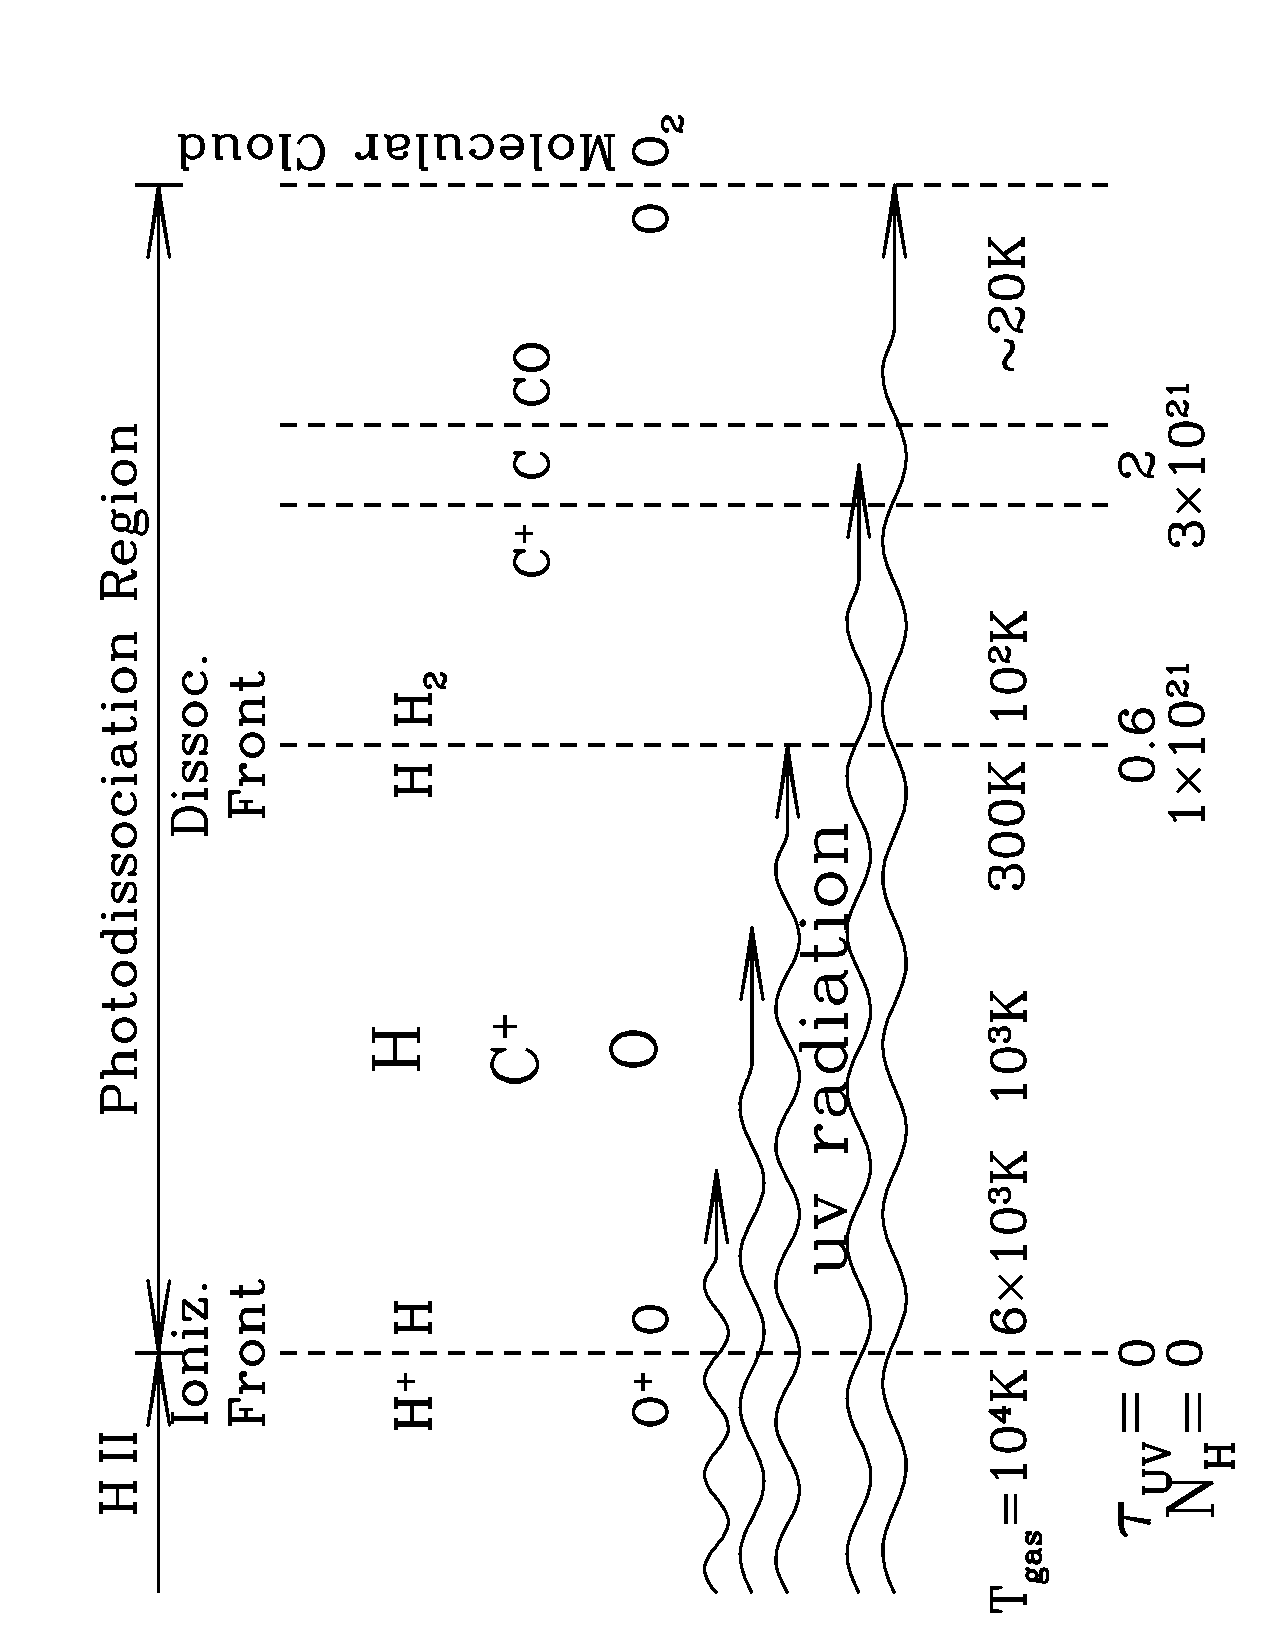
\includegraphics[angle=-90]{ism_figures/Draine-31_2}
\caption{A schematic of a photon-dominated region (Draine Figure 31.2).}
\end{marginfigure}
\begin{enumerate}
\item Dense cores: $n_{\Htwo{}} \gg 200 {\rm\, cm^{-3}}$. N$_2$H$^+$ is a popular choice for observing this phase (because it's not depleted onto dust grains).
\item Hot cores: After the protostar begins to shine, the dust is heated to $T \sim 100$ K, and often we have $n_{\Htwo{}} > 10^6 {\rm\, cm^{-3}}$. 

For low-temperature gas, charge transfer reactions take place:
\[{\rm XH^+ + HD \leftrightarrow XD^+ + H_2 +} \Delta E, \]
yielding abundances
\[n_{\rm XH^+} \cdot n_{\rm HD} = n_{\rm XD^+} \cdot n_{\rm \Htwo{}} \cdot \exp(-\Delta E/kT). \]
The righthand side of the reaction tends to dominate as \textit{deuteration} takes place and creates slightly more stable molecules. So we can measure timescales on the order of thousands of years this ways.
\item Photon-dominated regions (PDRs): UV photons from OB stars dominate chemistry and energy balance cause \textbf{fluorescent excitation}\sidenote{\Htwo{} fluorescence is due to UV photons exciting the electronic state, which then de-excites into a random vibro-rotational mode.} of \Htwo{} vibrational levels.

Cooling is mostly de to fine structure lines [\spec{C}{II}] 158 \um{}, [\spec{O}{I}] 63 \um{} (the latter of which is strong due to high density).
\end{enumerate}

\subsection{Magnetic fields}
There are four approaches to measuring magnetic fields:

First is \textbf{synchrotron emission} - if we assume a power-law energy distribution with spectral index $p$ ($N\,dE \propto E^{-p}\,dE$), we can measure the $B$ field strength from synchrotron intensity, $B$ field geometry from its linear polarization
\begin{equation}
\Pi = \frac{p+1}{p+7/3}.
\end{equation}

For example, a supernova remnant with $p=2$ gives $\Pi \sim 0.7$. But the measured polarization might be far lower, which tells us about how de-coherent the $B$ field direction may be (i.e., geometry).

Secondly, we can use \textbf{Faraday rotation}. Let's assume a plane wave propagating parallel to a fixed magnetic field, $B_0$, which give us circularly polarized waves with cyclotron frequency $\omega_B = eB_0/m_e c$. The electrons move with different velocities for different polarizations (right vs. left), as given by their dielectric constants:
\begin{equation}
\epsilon_{R,L} = 1 - \frac{\omega_p^2}{\omega(\omega \pm \omega_B)}.
\end{equation}
$\omega_p = 4\pi n_e e^2/m_e$ is the plasma frequency, and essentially indicates the electron mobility. Therefore the phase angle, $\phi$, will rotate different amounts for $R,L$ polarized emission.
\begin{equation}
\phi_{R,L} = \frac{1}{c}\int_0^L ds\, \omega\sqrt{\epsilon_{R,L}}.
\end{equation}

So, for a background, linearly polarized source, the phase angle will rotate by an angle
\begin{align}\label{eq:faraday rotation}
\Delta \phi &= \frac{1}{2}\int_0^L ds\,\left (k_R - k_L\right )\nonumber \\
&\approx \frac{2\pi e^3}{m_e^2 c^2 \omega^2}\int_0^L ds\, n B_0.
\end{align}
where the last step used a first-order Taylor expansion (because $\omega_p \ll \omega$; $\omega_p \sim$ kHz and observed $\omega \sim $ GHz). This latter integral is also called the \textbf{rotation measure}, or RM.

Keep in mind the following: 
\begin{itemize}
\item The magnitude of $\Delta \phi \propto \omega^{-2} \propto \lambda^2$. Observationally, we usually use $\geq 3$ wavelengths to break $\pm 2\pi$ degeneracies (two to measure $\Delta \phi$, and a third to break degeneracies).
\item We've assumed $B_0$ to be parallel to the propagation direction (so substitute $B_0 \rightarrow B_{||}$). The field can double back on itself, so Faraday rotation underestimates $B_{||}$ strength due to cancellations---particularly on small scales.
\item We only measure $\int n_e B_{||}\, ds$, so we can't break the degeneracy between $B_{||}$ and $n_e$ from Faraday rotation. To get around this degeneracy, we must measure Faraday rotation towards pulsars, where we can \textit{also} get the \textbf{dispersion measure} (DM).
\end{itemize}

So how do we calculate the dispersion measure? Ignoring the $B$ field for a moment, our dielectric constant is given by $\epsilon = 1 - (\omega_p/\omega)^2$, leading to the dispersion relation
\[c^2k^2 = \omega^2-\omega_p^2.\]

For frequencies below the plasma frequency, the $k$ wavenumbers are imaginary and those waves are damped exponentially. But they \textit{do} manifest in the group velocity, 
\[v_g = \frac{\partial \omega}{\partial k} = c\left (1-\left( \frac{\omega_p}{\omega}\right )^2 \right )^{1/2}.\]
The arrival of a given pulse, from a pulsar at distance $L$, is $t_p = \int_0^L ds\, v_g^{-1}$, where we can Taylor expand (again because $\omega_p \ll \omega$) to estimate 
\[t_p \approx \frac{L}{c} + \frac{1}{2c\omega^2}\int_0^L ds\, \omega_p^2.\]
Then taking the frequency derivative,
\begin{equation} \label{eq:dispersion measure}
\frac{\partial t_p}{\partial \omega} = -\frac{4\pi e^2}{m_e c \omega^3} \int_0^L ds\, n_e,
\end{equation}
and the dispersion measure, DM$ = \int_0^L ds\, n_e$. We should be able to plot the pulses from pulsars at different frequencies and find a simple $\omega^{-3}$ relation. Then, using equations \eqref{eq:faraday rotation} and \eqref{eq:dispersion measure}, we can make an average line-of-sight $B$ field
\begin{equation}
\ev{B_{||}} = \frac{\rm RM}{\rm DM} = \frac{\int_0^L ds\, n_e B_{||}}{\int_0^L ds\, n_e}.
\end{equation}

The rotation measure is formally defined:
\[\frac{\rm RM}{\rm rad\, m^{-2}} = 8.1\e{5} \int_0^L \frac{ds}{\rm pc}\, \left (\frac{B_{||}}{\rm Gauss}\right )\left (\frac{n_e}{\rm cm^{-3}}\right ).\]

Thirdly, we can use \textbf{polarization}. Let's go back and review the \textbf{Stoke's parameters}:
\begin{align}
I &=  E_1^2 + E_2^2\\
Q &=  E_1^2 - E_2^2\\
U &= 2E_1E_2\cos(\phi_1-\phi_2)\\
V &= 2E_1E_2 \sin(\phi_1-\phi_2)
\end{align}
These apply for \textit{single monochromatic waves} (and $I^2 = Q^2 + U^2 + V^2$). If the incident waves are \textit{quasi-monochromatic waves}, where the amplitudes/phases can drift slowly, then the time-averaged versions of the Stoke's parameters above are valid, and $I^2 \geq Q^2 + U^2 + V^2$ and we define the polarization
\begin{equation}
\Pi = \frac{\sqrt{Q^2 + U^2 + V^2}}{I}.
\end{equation}

So we write the \textbf{Stoke's vector} as a sum of unpolarized and polarized components:
\begin{equation}
\begin{pmatrix}
I\\Q\\U\\V
\end{pmatrix} =
\begin{pmatrix}
I-\sqrt{Q^2 + U^2 + V^2}\\0\\0\\0
\end{pmatrix} +
\begin{pmatrix}
\sqrt{Q^2+U^2+V^2}\\Q\\U\\V
\end{pmatrix}.
\end{equation}

Observationally, dust causes
\begin{itemize}
\item[-] Polarized extinction of background stars (comes from everywhere, low value)
\item[-] Polarized emission (dominated by \textit{large} grains in \textit{dense} clouds)
\end{itemize}
Draine Figure 21.3 shows a map of the Galactic dust polarization. But to actually estimate $B$, we can follow the method of Chandrasekhar \& Fermi (1953): assume that the gas velocity dispersion is driven at the \textbf{Alfv\'en speed}, $v_A = B/\sqrt{4\pi \rho}$. It's the speed at which a transverse wave propagates through a magnetic field with oscillations $y = a\cos k (x-v_A t)$. Then, by differentiating the oscillation displacements with distance and time, we find
\begin{align*}
y' =\frac{dy}{dx} &= -ak \sin k(x-v_At)\\
\dot y =\frac{dy}{dt} &= - akv_A \sin k(x-v_At),
\end{align*}
so that \begin{align*}
v_A^2\, y'^2 &= \dot y^2\\
v_A^2 \sigma^2 &= \frac{1}{3}v^2,
\end{align*}
where $\sigma$ is the rms polarization angle and $v$ is the rms velocity of the gas. Thus, we can finally solve (assuming that the turbulent velocity is driven at the Alfv\'en speed):
\begin{equation}
B = \frac{v}{\sigma} \left (\frac{4\pi \rho}{3}\right )^{1/2}.
\end{equation}


\section{Friday, 30 October}
% HW for next Tuesday: read Draine ch 41
\subsection{Magnetic fields: the Zeeman effect}

\begin{marginfigure}
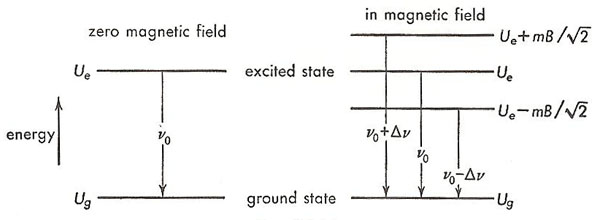
\includegraphics{ism_figures/zeeman_effect}
\caption{The Zeeman Effect in neutral hydrogen. The higher frequency line emission will be circularly polarized, the original frequency line emission will be linearly polarized parallel to $\vec B$, and the lower frequency line emission will be oppositely circularly polarized.}
\end{marginfigure}
For a neutral atom, the ground state of $\vec F = \vec J + \vec I$, where $F$ is the total magnetic moment, and $I$ is the nuclear spin. In \HI{}, the ground state has $F = J + 1 = 1$ (0), with corresponding $2J+1 = 3$ (1) degeneracy. In an external magnetic field, $U \propto - \vec F \cdot \vec B$, and so for $F=1$, we see a very small splitting in the 21-cm line, due to the magnetic field breaking the degeneracy.
\begin{itemize}
\item[] If the line of sight is parallel to $\vec B$, then the unsplit (middle energy) line will be missing, and split lines will be completely polarized.
\item[] If the line of sight is perpendicular, then all three lines are observable, and split lines will be linearly polarized perpendicular $\vec B$.
\item[] For a general line of sight, the split lines will have elliptical polarization.
\end{itemize}

The splitting strength is proportional to $|\vec B|$; for \HI{} the two split lines are separated by a frequency
\[\Delta \nu_B = \frac{eB_{||}}{2\pi m_e c} = 2.8\e{6} \left (\frac{B}{\rm Gauss}\right ) \,\textrm{Hz}.\]

For general molecules and atoms, the split levels of identical $J$ is given by
\begin{align}
U &= \frac{\mu_B}{\hbar}\left (g_L \vec L + g_S \vec S\right ) \cdot \vec B \nonumber \\
&\approx \frac{\mu_B}{\hbar}\left (\vec J + \vec S\right )\cdot \vec B,
\end{align}
where we have assumed $g$ factors $g_L = 1$, $g_s=2$. In terms of the \textit{Land\'e $g$ factor},
\begin{equation}
g(L,S,J) = \frac{J(J+1) + S(S+1) - L(L+1)}{2J(J+1)},
\end{equation}
and the $J$ value, we can find the average magnetic energy
\begin{equation}
\ev{U} = \frac{1}{2}\left (\frac{e\hbar B_{||}}{m_e c}\right )g M_J.
\end{equation}

So the frequency of newly split transitions are
\begin{equation}
\omega_{12} = \frac{1}{2}\left (\frac{eB_{||}}{m_e c}\right )\left (g_1 M_{J_1}-g_2 M_{J_{2}}\right ).
\end{equation}
Observationally, we can use the \textit{polarized} spectra, and take the \textbf{difference spectrum} of the right and left circularly polarized emission to quantify the field strength.\sidenote{Empirically, we see that $B \propto n_H^{1/2}$ for $n_H \geq 10 \,\textrm{cm}^{-3}$. It also turns out that the Alfv\'en speed is $v_A \propto B/\sqrt{\rho} \sim 1.85 {\,\rm km\,s^{-1}}$, and that this velocity is close to the observed linewidths. Therefore, the motions in molecular clouds seem to be manifest from large-scale MHD waves.}

The median field strength as found in difference absorption spectra via Zeeman splitting of the 21-cm line is $B \sim 6\, {\m G}$, implying that the magnetic pressure is several times greater than that of the gas pressure!

\subsection{Star formation: observational constraints}
\begin{itemize}
\item[] Stars form from dense molecular gas, which is traced by the correlation between HCN (1-0) line and FIR continuum.
\item[] Stars form in lots of binaries ($\sim 2/3$ of stars are in binaries).
\item[] Stars tend to form in embedded clusters.
\item[] Stars do \textit{not} form via free-fall collapse of gas.\sidenote{The free-fall time scale is \begin{equation}t_{\rm ff} = \left (\frac{3\pi}{32 G \rho}\right )^{1/2}. \end{equation} In the Milky Way, $t_{\rm ff} \sim 4.3\e{7}\sqrt{(n_H/\textrm{cm}^{-3})}$ yr.}
\item[] Stars do not form with a Salpeter IMF down to $0.1\,M_\odot$. A better modern IMF, $\Phi(m)$ is given by Kroupa et al. (1993) or Chabrier et al. (2003).
\item[] The mass function of dense cores has a power-law index ($\propto m^{-2.5}$) similar to the that of the IMF for CO-emitting clouds ($\propto m^{-1.7}$).
\begin{marginfigure}
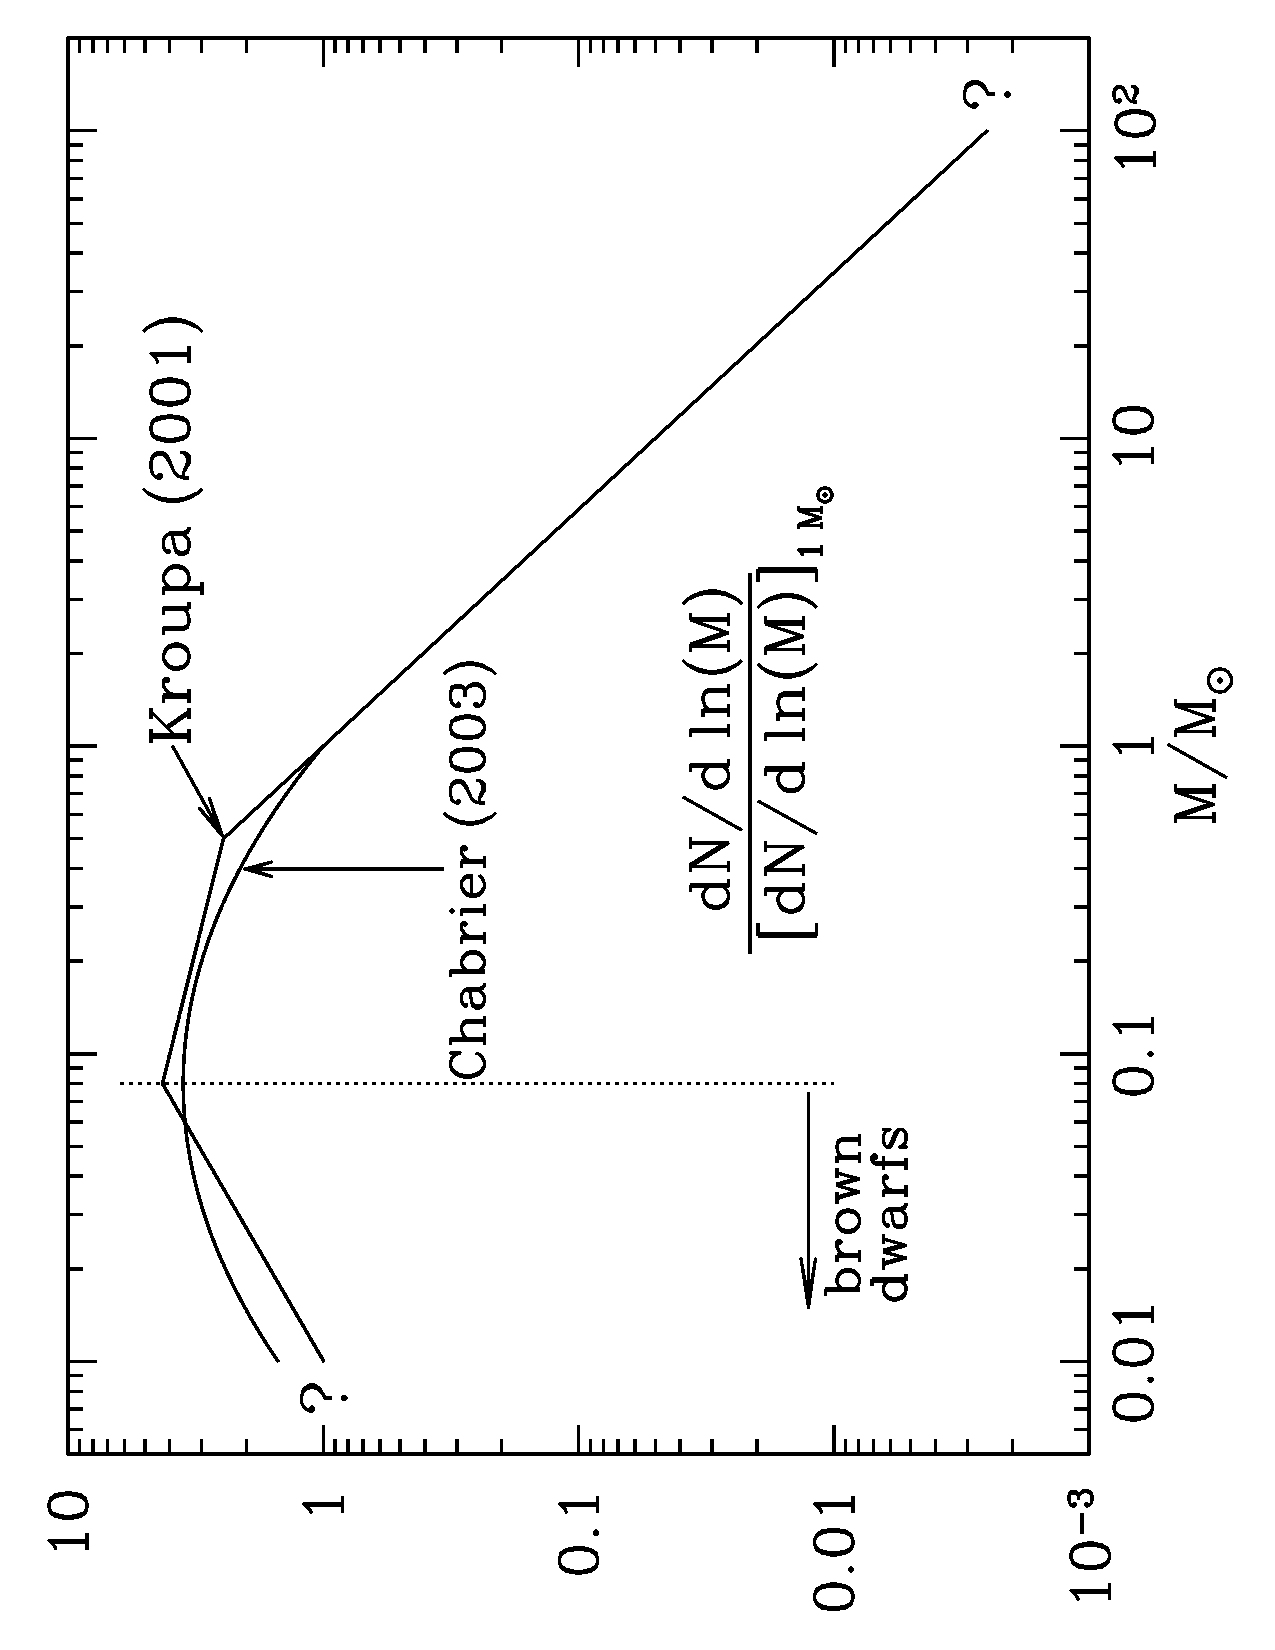
\includegraphics[angle=-90]{ism_figures/Draine-42_1}
\caption{A few forms of the initial mass function (Draine Figure 42.1).}
\end{marginfigure}
\item[] The efficiency of star formation (SF) is $1-3\%$ of GMC mass into stars, and $10-20\%$ of dense gas mass into stars.
\item[] Protostars grow from the difference between accretion (inflow) and outflow. We can trace the outflow via SiO emission.
\end{itemize}

The observational classification of young stars are
\begin{itemize}
\item[] \textbf{Class 0} have more than half of their mass in infalling envelopes, but are too heavily obscured to have optical counterparts
\item[] \textbf{Class I} have less than half of their mass infalling, have strong evidence of outflows, and have IR (and sometimes optical) counterparts
\item[] \textbf{Class II} have dissipated envelopes, but still have circumstellar disks; are also called \textbf{\textit{classical} T Tauri stars}
\item[] \textbf{Class III} have dispersed the inner edge of protostellar disks (due to radiation); are also known as \textbf{\textit{weak-lined} T Tauri stars}
\end{itemize}

To understand the star formation process better (since it's not as simple as computing the free fall of gas), we'll delve into fluid mechanics
\subsection{Basic equations of fluid mechanics}

We will begin by deriving the equations for conservation of mass, momentum, and energy. First ups is \textit{conservation of mass}. We'll consider a small volume $\mathcal V$ bounded by a surface $\mathcal S$, and a change of density within $\mathcal V$ as a function of time $\frac{\partial \rho}{\partial t}(\vec x,t)$. The mass flux is $\rho \vec v$ for a velocity field $\vec v(\vec x,t)$.
\begin{align}
\label{eq:continuity}
\frac{\partial}{\partial t} \int_{\mathcal V} dV\, \rho + \int_{\mathcal S} d\Sigma\, \rho \vec v \cdot \hat n &= 0\nonumber \\
\int_{\mathcal V} dV\, \left (\frac{\partial \rho}{\partial t} + \vec \nabla \cdot (\rho \vec v)\right ) &= 0 \nonumber \\
\frac{\partial \rho}{\partial t} + \vec \nabla \cdot (\rho \vec v) &=0.
\end{align}
This is also called the \textit{continuity equation}. We can also write this as a \textbf{convective} (or \textbf{Lagrangian}) \textbf{derivative}:
\begin{equation}
\frac{d\rho}{dt} = \frac{\partial \rho}{\partial t} + \vec v \cdot \vec \nabla \rho = -\rho \vec \nabla \cdot\vec v,
\end{equation}
where $\vec v \cdot \vec \nabla \rho$.\sidenote{The Lagrangian derivative is evaluated by following a fluid element, whereas the Eulerian derivative is evaluated at a fixed location.}


\section{Tuesday, 3 November}
\subsection{Basic equations of fluid mechanics (continued}
The momentum flux crossing a differential surface element, $d\Sigma$ is $(\rho \vec v \cdot \hat n d\Sigma)\vec v$. Then, the equation of momentum conservation can be found (similarly to last time):
\begin{align}
\frac{\partial}{\partial t}\int_{\mathcal V} dV\, \rho \vec v + \int_{\mathcal S} d\Sigma \left (\hat n \cdot \rho \vec v\right ) \vec v &= 0 \nonumber\\
\frac{\partial}{\partial t} \int_{\mathcal V} \left [dV \, \rho \vec v +  \vec \nabla \cdot \left (\rho \vec v \otimes \vec v \right )\right ] &= 0 \nonumber\\
\frac{\partial (\rho \vec v)}{\partial t} + \vec \nabla \cdot  \mathbf{T_{\rm mo}} &= 0,
\end{align}
where $\mathbf{T_{\rm mo}} = \rho \vec v \otimes \vec v$ is the \textit{momentum flux in tensor form}. 

However, now we can add surface stress via a term $\mathbf{T_{\rm surf}}(i,j)$, which is the force per area in direction $i$ across surface area normal to direction $j$. Using Gauss's law again, 
\begin{equation}
\int_{\mathcal S}d\Sigma_j \, \left (\hat n \cdot \mathbf{T_{\rm surf}}(i,j)\right ) = \int_{\mathcal V} dV\, \left (\vec \nabla_j \cdot \mathbf T_{\rm surf}(i,j)\right ).
\end{equation}
So then, our pressure term can be found
\[-\vec \nabla P = \vec \nabla \cdot \mathbf T_{\rm surf}(i,j),\]
and we can additionally include a force per volume $-\rho \vec \nabla \Phi$,\sidenote{This might be from a potential $\Phi$---which might be gravity, for example. We're ignoring things like viscosity, or magnetic fields.} and end up with the full equation of momentum conservation
\begin{equation}
\label{eq:momentum conservation}
\frac{\partial (\rho \vec v)}{\partial t} + \vec \nabla \cdot \mathbf T_{\rm mo} = -\vec \nabla P - \rho \vec \nabla \Phi.
\end{equation}

Were we to set the left-hand side of equation \eqref{eq:momentum conservation} to zero, then we have hydrostatic equilibrium (i.e., pressure is balanced by gravity), and the fluid remains motionless. Now we add a body force (i.e., a magnetic field, $\vec B$) in a nonzero charged particle density (i.e., current, $\vec j$),\sidenote{Recall that $\vec \nabla \cdot \vec B = 0$ and $\vec j = \frac{1}{4\pi}\vec \nabla \times \vec B$.} and find in terms of the metric, $\mathbf g$, the \textbf{Navier-Stokes equation} for zero viscosity:
\begin{equation}
\label{eq:Navier-Stokes}
\frac{\partial(\rho \vec v)}{\partial t} + \vec \nabla \cdot \left (\mathbf T_{\rm mo} + \mathbf T_{\rm mag} + \mathbf g P\right ) = -\rho \vec\nabla \Phi.
\end{equation}
The magnetic tensor is simply defined
\[\mathbf T_{\rm mag} = \frac{B^2}{8\pi}\mathbf g - \frac{\vec B \otimes \vec B}{4\pi}.\]


For \textit{conservation of energy density}, we multiply equation \eqref{eq:continuity} by $v^2/2$ and take the dot product of equation \eqref{eq:momentum conservation}. Additionally, we define the internal energy $u$ (e.g., heat), the entropy $s$, and enthalpy $h = (u+P)/\rho$:
\begin{equation}
\label{eq:energy density conservation}
\frac{\partial}{\partial t}\left [\rho \left (\frac{1}{2}v^2 + u + \Phi\right ) + \frac{B^2}{8\pi}\right ] + \vec \nabla \cdot \left [\rho \vec v\left (\frac{1}{2}v^2 + h + \Phi\right)\right ] + \frac{1}{4\pi}\vec E \times \vec B = \rho T \frac{ds}{dt}.
\end{equation}

\subsection{The Jeans instability}
Firstly, let's assume $\vec B = 0$, and we can treat the density and velocities as \textit{perturbations} to their equilibrium quantities: $\rho = \rho_0 + \rho_1$ and $\vec v = \vec v_0 + \vec v_1$.\marginnote{It will be useful to invoke the vector identity \begin{equation}
\vec \nabla \cdot (\rho \vec v) = \vec v \cdot \vec \nabla \rho + \rho (\vec \nabla \cdot \vec v).
\end{equation}} Using the continuity equation (equations 14-15 from the Lecture 18 equation sheet), we take the difference between the total and the equilibrium quantities of $\partial \rho/\partial t$ in order to find equation (16). Equation (17) is found via perturbing the potential, $\Phi = \Phi_0 + \Phi_1$ and substituted $dP \simeq c_s^2\, d\rho$. Using Poisson's law ($\nabla^2 \Phi_1 = 4\pi G\rho_1$), and assuming \textit{constant} $\rho_0$ and zero initial velocity ($v_0 = 0$), we find perturbed quantities
\begin{align*}
\frac{\partial \rho_1}{\partial t} &= -\rho_0 \vec \nabla \cdot \vec v_1\\
\frac{\partial \vec v_1}{\partial t} &= -\vec\nabla\Phi_1 - \frac{c_s^2}{\rho_0}\vec \nabla\rho_1.
\end{align*}
We take the divergence of the latter equation,
\begin{equation}
\frac{\partial (\vec \nabla\cdot \vec v_1)}{\partial t} = -4\pi G\rho_1 - \frac{c_s^2}{\rho_0}\nabla^2\rho_1,
\end{equation}
and recognize that the term $\vec\nabla \cdot \vec v_1$ can be substituted with the former equation:
\begin{equation}
\frac{\partial^2 \rho_1}{\partial t^2}= -4\pi G\rho_0 \rho_1 - c_s^2\nabla^2\rho_1.
\end{equation}

If the perturbation propagates as a plane wave ($\rho_1 \propto e^{-i(\omega t - kx)}$), then it is subject to a dispersion relation
\begin{equation}
\omega^2 = c_s^2 \left [k^2 - \left (\sqrt{4\pi G\rho_0}/c_s\right )^2\right ].
\end{equation}

When $k < \sqrt{4\pi G\rho_0}/c_s$, $\omega$ is imaginary, and the perturbations will have an exponentially growing and damping mode. Throwing out the damped solution, we see how our instabilty grows exponentially. The critical wavenumber, $k_*$, corresponds to a length scale (inversely); this is called the \textbf{Jean's length}:\sidenote{We've snuck in the sound speed $c_s^2 = \gamma k_BT/\mu m_H$.}
\begin{equation}
L_J = \frac{2\pi}{k_{*}} = \sqrt{\frac{\pi \gamma k_B T}{\mu m_H G\rho_0}},
\end{equation}
or an equivalent \textbf{Jean's mass}:
\begin{equation}
M_J = \rho_0 L_J^3 = \left (\frac{\pi \gamma k_B T}{\mu m_H G}\right )^{3/2} \rho_0^{-1/2}.
\end{equation}
This is expressed as a \textit{thermal} Jean's mass, at which gravitational energy exceeds thermal energy.

Using typical values ($\mu \simeq 2, \gamma = 3/5$), we find
\[\frac{M_J}{M_\odot} = 1.2 \left (\frac{T}{\rm 10\, K}\right )^{3/2} \bigg (\frac{n_0}{10^3\rm\, cm^{-3}}\bigg )^{-1/2},\]
suggestive of the importance of the Jean's criterion in star formation, seeing as this mass is close to that of our Sun.


\subsection{Magnetic fields and star formation}
The free-fall timescale is too short to be physically plausible, because it's solely based on the thermal pressure. We will invoke the magnetic pressure to help slow down gravitational free fall.

For a uniform sphere, the gravitational binding energy is $U_G = 3GM^2/5R$, and the magnetic energy content is $U_B = \int dV B^2/8\pi = B^2R^3/6$. If we set these equal, the back-of-the-envelope critical magnetic mass turns out to be
\[M_{\rm crit} = \left (\frac{5}{18 G}\right )^{1/2} BR^2 \simeq 0.17 \frac{\Phi_B}{\sqrt{G}},\]
where the magnetic flux is $\Phi_B = \pi BR^2$. For typical systems in the ISM, this critical mass is \textit{larger} than the Jeans mass---so that magnetic fields actually provide support against collapse, rather than thermal pressure.

For subcritical cloud masses, \textbf{ambipolar diffusion}--where neutral and ionized material slip past each other and the $B$ field diffuses outwards--allows less massive stars to collapse. The ambipolar diffusion timescale is $t_{\rm ambi} \sim 10^6$ yr cf. $t_{\rm ff}\sim 10^4$ yr.

\section{Friday, 6 November}
% Read Draine chapter 38,39
% SALT proposals due Nov 20

\subsection{Magnetic fields and star formation (continued)}
As protostars collapse, angular momentum conservation leads to rotational support against gravitational instability. The rotating gas cloud has $E_{\rm grav} \sim - GM^2/R$ and $E_{\rm rot} \sim J^2/2I = 5J^2/4MR^2$ (for a constant density sphere). Contraction will stop when these energies roughly balance each other, at 
\[R_{\rm min} \sim \frac{5}{4}\frac{J^2}{GM^3}.\]

This can cause the protostellar disk to shrink by one or maybe two orders of magnitude, but nowhere near the many orders of magnitude needed to actually create a star. The catalyst for collapse is the magnetic field. The cloud will collapse along (e.g., parallel to) the $B$ field lines to make a pancake shape, and twist the $B$ field lines to corotate in the ambient gas. This is described in Draine \textsection 41.5, and can be quantified with a \textbf{magnetic spin-down timescale} of $t_B \sim 8000$ yr. The magnetic spin-down timescale is always shorter than the contraction timescale, which means that the $B$ fields can robustly transfer angular momentum from the system and allow for collapse.

\subsection{Shocks}
A shock is a pressure-driven disturbances travel faster than the signal speed, or \textbf{magnetosonic speed}\sidenote{On Earth, we think about sonic booms and such, but if a magnetic field allows for signal propagation, then we should care about the magnetosonic speed. The magnetosonic speed is simply the sum of the sound speed and Alfv\'en speed: 
\begin{equation}
c_{\rm ms}^2 = \frac{\gamma P}{\rho} + \frac{B^2}{4\pi \rho}.
\end{equation}} and increase the entropy of the fluid through which they pass. 

There are two ways to produce shocks. The first way is by the steepening of a (finite-amplitude) sound wave, if $\gamma = c_P/c_V > 1$. Another way is via supersonic compressive perturbations (e.g., like a supersonic jet or the crack of a whip). Below, in Fig \ref{fig:shocks}, some relevant quantities are plotted against position. Note that we work in the shock frame, so that the shock is moving to the right.


\begin{figure}
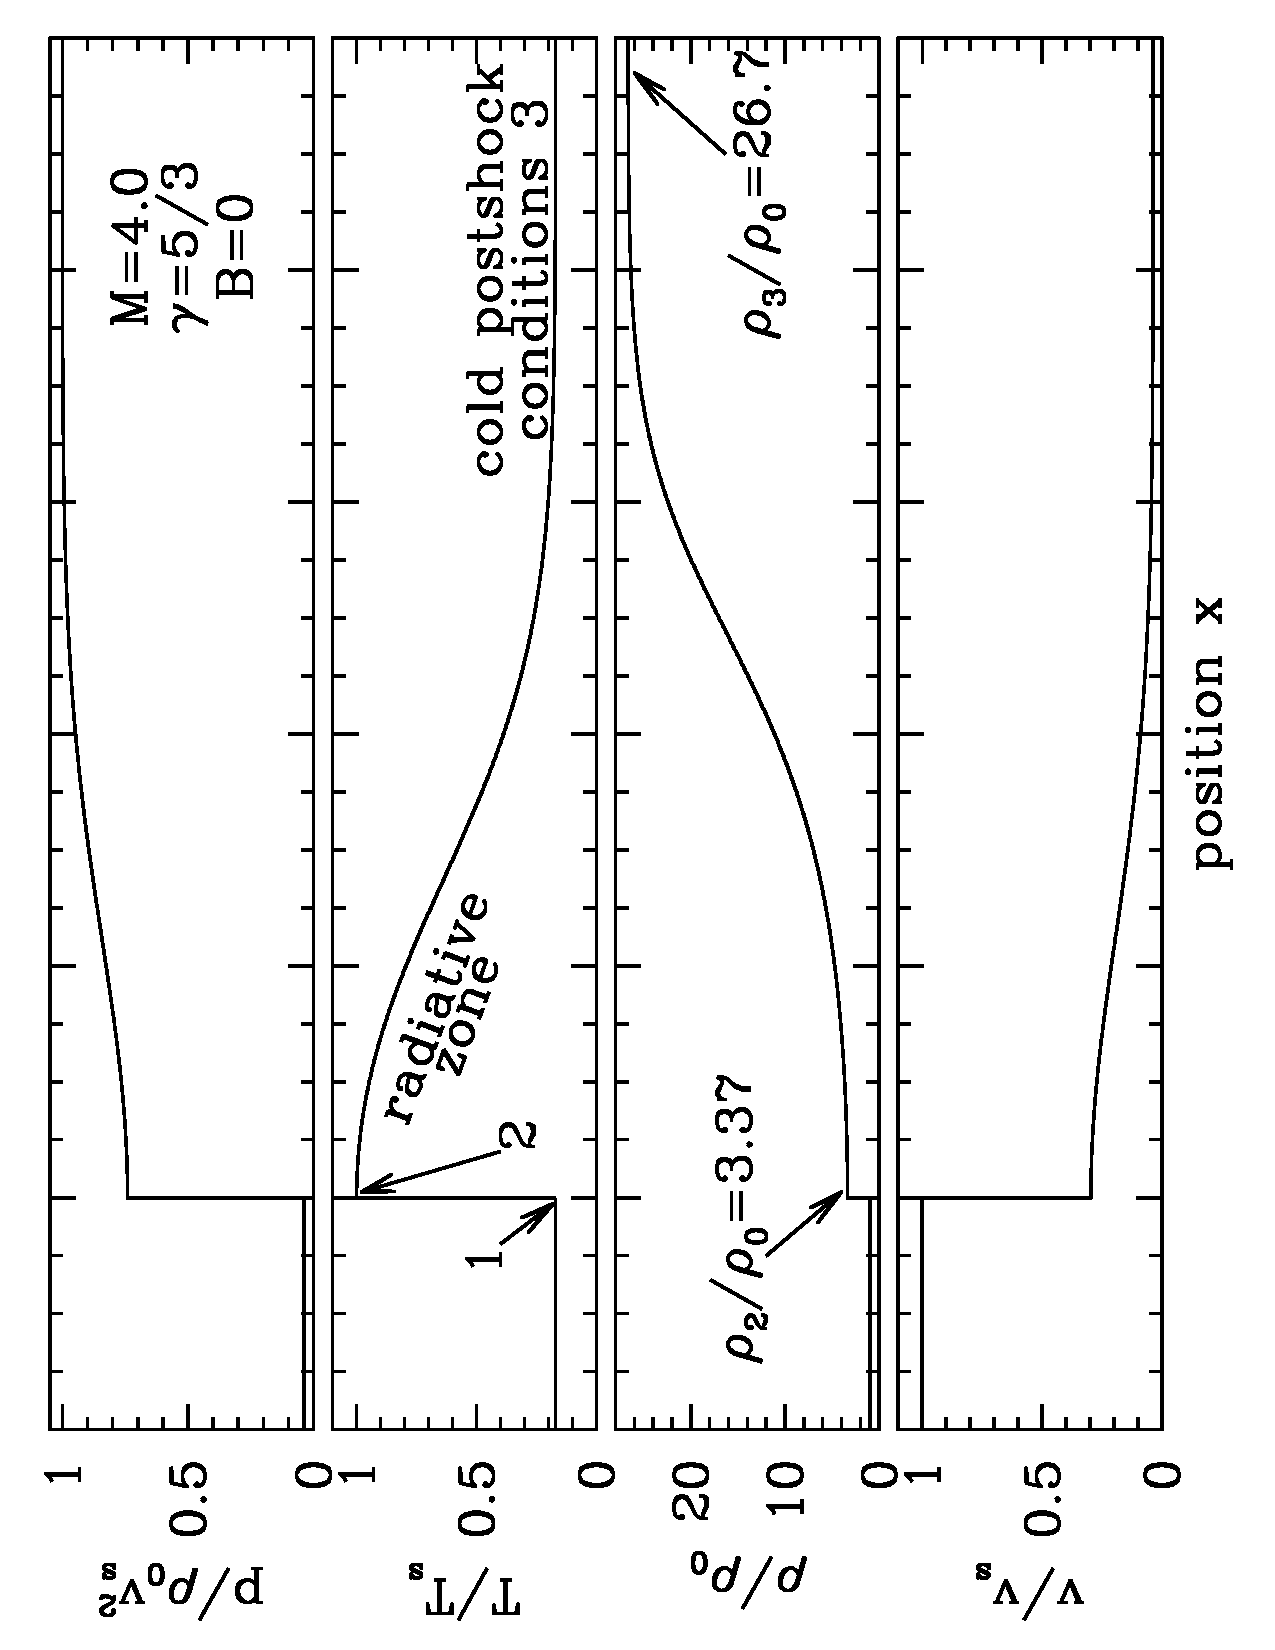
\includegraphics[width=0.75\columnwidth, angle=-90]{ism_figures/Draine-36_1}
\caption{The pressure, temperature, density, and fluid velocity (in the shock frame) of a \textit{J-type} shock (Draine Figure 36.1).}
\label{fig:shocks}
\end{figure}


In the ISM, shocks can be generated by SN explosions, stellar winds, gas cloud collisions, pressure-driven expansion of an \HII{} region, infall of material onto a cloud, or dynamical cloud perturbations (e.g., a spiral shock)---to give a few examples.

\begin{marginfigure}
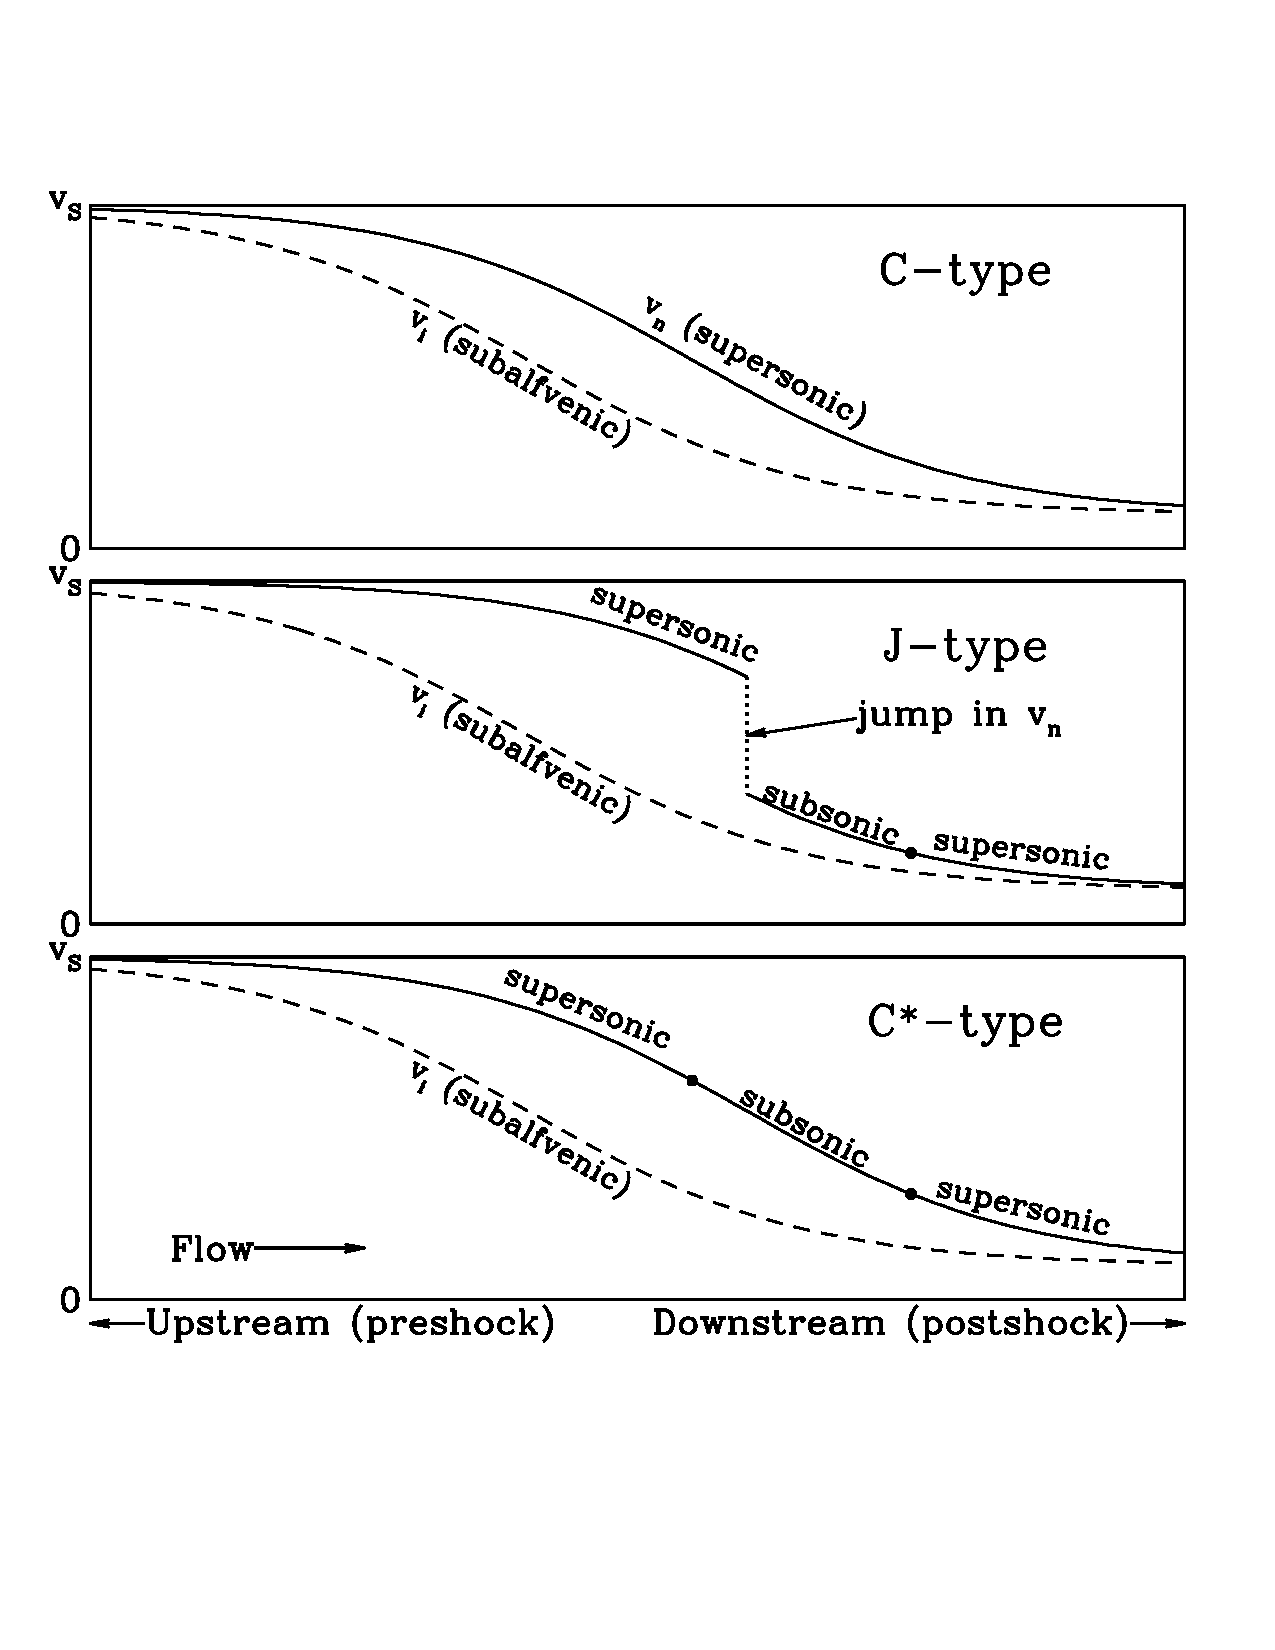
\includegraphics[]{ism_figures/Draine-36_4}
\caption{The velocity gradient over C-type (and C*-) and J-type shocks (Draine figure 36.4).}
\end{marginfigure}

There are two categories of shocks, which are shown in the figure to the right (Draine figure 36.4):
\begin{enumerate}
\item \textbf{J-type} (jump): The gas stops suddenly, is heated to high temperatures, and there is very little relaxation. The shock front is much thinner than the post-shock relaxation layer. 
\item \textbf{C-type} (continuous): These (weaker) shocks tend to occur in magnetized gas that have a low ionization fraction. Heating and cooling are balanced and determine the temperature in the C-shock.
\end{enumerate}
Within molecular clouds, shocks with $v < 40 {\rm\, km\, s^{-1}}$ are likely C-type shocks, and with $v > 40 {\rm\, km\, s^{-1}}$ are likely J-type shocks.


To model our shock, we will work in a shock frame, and assume an infinite plane geometry. The fluid moves in the $\hat x$ direction. Quantities with a $0$ subscript are pre-shock, and quantities with a $1$ subscript are post-shock.

We will calculate the \textbf{jump conditions} across a J-type shock. Starting with the continuity equation (or Equation \ref{eq:continuity}), we note that the shock is stationary in the shock frame, so that
\[\frac{\partial \rho}{\partial t} = 0,\textrm{\ and\ that\ } \vec\nabla \cdot (\rho \vec v) = \frac{\partial}{\partial x} (\rho v_x) = 0.\]

We then integrate from pre- to post-shock, finding that
\[ 0 = \int_{\rm pre}^{\rm post} dx\, \frac{\partial}{\partial x}(\rho v_x) = \left (\rho v_x\right )_1 - \left (\rho v_x\right )_0,\]
\begin{equation}
\rho_0 v_0 = \rho_1 v_1.
\end{equation}
This is the mass conservation across the shock. The momentum flux is conserved by examining
\[\rho \frac{d \vec v}{dt} = - \vec \nabla \left ( P + \frac{B^2}{8\pi}\right ) + \frac{1}{4\pi}\left (vec B \cdot \vec \nabla\right ) \vec B - \rho \Phi,\]
which ignores the viscosity on both sides of the shock. Details are shown in equations (10-14) of the Lecture 19 equation sheet--note that we've used the product rule and that $\frac{\partial}{\partial x}(\rho v_x) = 0 $ to derive equation (13). If we assume a small (negligible) change in gravity across the shock, then the right-hand side of equation (12) is zero, so that
\begin{equation}
\rho_0 v_0^2 + P_0 + \frac{1}{8\pi}\left (B_{y_0}^2 + B_{z_0}^2\right ) = \rho_1 v_1^2 + P_1 + \frac{1}{8\pi}\left (B_{y_1}^2 + B_{z_1}^2\right ).
\end{equation}
Finally, to conserve energy, we start with equation \eqref{eq:energy density conservation}, and ignore $\frac{\partial \Phi}{\partial x}$ and radiative heating and cooling, heat conduction, and substitute
\[u = \frac{1}{\gamma -1}P \hspace{3em} h = \frac{\gamma}{\gamma-1}P,\]
to derive (with no derivation--sorry!)
\begin{equation}
\frac{1}{2}\rho_0 v_0^3 + \frac{\gamma}{\gamma-1} v_0 P_0 + v_0 \frac{B_0^2}{8\pi} = \frac{1}{2}\rho_1 v_1^3 + \frac{\gamma}{\gamma-1} v_1 P_1 + v_1 \frac{B_1^2}{8\pi}.
\end{equation}
These three are the Rankine-Hugonoit jump conditions. Additionally, we have an equation for magnetic flux conservation derived from conserving
\[\frac{\partial \vec B}{\partial t} = - \vec \nabla \times (\vec v \times \vec B),\]
so that \begin{equation}
\vec v_0 \times \vec B_0 = \vec v_1 \times \vec B_1.
\end{equation}
If the magnetic field is \textit{perpendicular to} the propagation of the shock, then clearly (recalling again that we're in the shock front) we derive that $v_0B_0 = v_1B_1$.


To consolidate, we have our four quantities $\rho, B, P, v$, and we have these four equations of conservation. Our shock equation solution is nontrivial if $v_0^2 > c_{\rm ms}^2$, of course. Let's define a compression factor
\begin{equation}
\xi \equiv \frac{\rho_1}{\rho_0} = \frac{B_1}{B_0} = \frac{v_0}{v_1},
\end{equation}
where we're collapsing the magnetic flux conservation and continuity equations to get this definition.

We are left with the remaining two equations:
\[\rho_0 v_0^2 + P_0 + \frac{B_0^2}{8\pi} = \rho_0 v_0^2 \frac{1}{\xi} + P_1 + \frac{B_0^2}{8\pi}\xi^2\]
\[\frac{1}{2}\rho_0v_0^3 + \frac{\gamma}{\gamma-1} v_0 P_0 + v_0\frac{B_0^2}{8\pi} = \frac{1}{2}\rho_0v_0^3 \frac{1}{\xi^2} + \frac{\gamma}{\gamma-1} v_0 P_1 \frac{1}{\xi} + v_0 \frac{B_0^2}{8\pi}\xi.\]

We can define a \textbf{dimensionless Mach number}, $\mathcal M$,
\begin{equation}
\mathcal M^2 \equiv \frac{v_0}{(\gamma P_0/\rho_0) + (B_0^2/4\pi \rho_0)}.
\end{equation}
In the limit of $B\rightarrow 0 $, $\mathcal M \rightarrow \mathcal M_s = v_0/c_s$, and in the limit of $P\rightarrow 0$, $\mathcal M \rightarrow \mathcal M_A = v_0 / v_A$. 

In the limit of $B \rightarrow 0$:
\[\frac{P_1}{P_0} = \frac{2\gamma}{\gamma+1} \mathcal M_s^2 - \frac{\gamma - 1}{\gamma + 1}\]
\[ \frac{\rho_0}{\rho_1} = \frac{\gamma-1}{\gamma+1} + \frac{2}{\gamma+1} \frac{1}{\mathcal M_s^2}.\]

For a very strong shock, $\mathcal M_s \gg 1$. Then (assuming an atomic gas with $\gamma = 5/3$), we can find that $\xi = 4$ (follow equations 32-35 on the lecture notes).


\section{Friday, 13 November}
% Refer to Draine chapter 38 for stellar winds
% But we're skipping straight to SN remnants

\subsection{Supernova remnants}
The evolution of a supernova remnant occurs in three phases:
\begin{enumerate}
\item The \textbf{free expansion phase} when the swept up mass is negligible compared to the ejected mass ($M_{\rm ejecta} \sim 1-5\,M_\odot$): $M_{\rm swept} \ll M_{\rm ejecta}$. We then get a blastwave moving outward at a constant velocity:
\[v_0 = \left (\frac{2E_0}{M_{\rm ejecta}}\right ) = 10^4 {\rm km\, s^{-1}}\left (\frac{E_0}{10^{51}\,\rm erg}\right )^{1/2}\left (\frac{M_{\rm ejecta}}{M_\odot}\right )^{-1/2}.\]
These speeds are highly supersonic--resulting in a jump shock--but there's so little material for it to do much at early stages. The free expansion phase ends when $M_{\rm ejecta} \sim M_{\rm swept}$, at a radius
\[R_1 \simeq \left (\frac{3M_{\rm ejecta}}{4\pi \rho_0}\right )^{1/3} = 2.4 \textrm{\, pc} \left (\frac{M_{\rm ejecta}}{M_\odot}\right )^{1/3}\left (\frac{n_H}{0.5\, \rm cm^{-3}}\right )^{-1/3}.\]

The thickness of the swept--up shell is estimated by using conservation of mass, or
\[\frac{4\pi}{3}R_1^3 \rho_0 = 4\pi R_1 \Delta R_1 \rho_1\]
\[\frac{\Delta R_1}{R_1} = \frac{\rho_0}{3\rho_1} = \frac{1}{12},\]
where we recall that $\xi=4$ for jump shocks and $\gamma = 5/3$. The time at which $R_1$ is reach is simply $t_1 = R_1/v_0 \approx 240 {\,\rm yr}$.

\item Next is the \textbf{adiabatic expansion}\sidenote{The shock is rather abrupt, and is irreversible (entropy increases), so that ``adiabatic'' is a poor description of this phase.} or \textbf{Sedov-Taylor phase}. Material can't cool efficiently (via radiation) because of the hot temperatures within the shock, so that the kinetic + internal thermal energy of gas is conserved.

The kinetic energy during the Sedov-Taylor phase is
\begin{equation}
E_{\rm kin} = \frac{1}{2}\int_0^{R_s}dR\, 4\pi R^2 \rho v^2 = \frac{2\pi}{3} R_s^3 \rho_0 v_s^2 \phi_{\rm kin},
\end{equation}
where obviously these quantities in the integral are not spatially constant, so that we introduce a fudge factor, $\phi_{\rm kin}$. Also, the swept-up mass is becoming increasingly important compared to $M_{\rm ejecta}$.
The internal energy is
\begin{align}
E_{\rm int} &= \int_0^{R_s} dR\, 4\pi R^2 \frac{P}{\gamma - 1}\nonumber \\
&= \frac{4\pi}{3} R_s^3 v_s^2 \frac{P_1}{\gamma - 1} \phi_{\rm int} \nonumber \\
&= \frac{4\pi}{3}R_s^3 \rho_0 v_s^2 \frac{2}{\gamma^2 - 1}\phi_{\rm int},
\end{align}
where we've introduced another fudge factor, and $P_1 = 2\rho_0 v_s^2 / (\gamma + 1)$. The ratio of kinetic-to-internal energy is $E_{\rm kin}/E_{\rm int} = (\gamma^2-1)\phi_{\rm kin}/4\phi_{\rm int}$, and the conservation of total energy results in
\[R_s^3 v_s^2 = \frac{2E_0}{2\pi \rho_0 }\left (\phi_{\rm kin} + \frac{4}{\gamma^2 - 1}\phi_{\rm int}\right )^{-1}.\]

But because $v_s = \dot R_s$, let's define a term
\[\xi_0 \equiv \frac{75}{8\pi}\left (\phi_{\rm kin} + \frac{4}{\gamma^2 - 1}\phi_{\rm int}\right )^{-1},\]
to derive
\begin{align}
R_s^3 \dot R_s^2 &= \left (\frac{2}{5}\right )^2 \xi_0 \frac{E_0}{\rho_0} \nonumber \\
R_s(t) &= t^{2/5} \left (\frac{\xi_0 E_0}{\rho_0}\right )^{1/5}\\
v_s(t) &= \frac{2}{5}t^{-3/5}\left (\frac{\xi_0 E_0}{\rho_0}\right )^{1/5}.
\end{align}

So now we have our shock speed evolving over time.

To get the temperature inside the bubble, we can apply the ideal gas law ($P = \rho k T/ \mu m_H$) to the post-shock gas:\marginnote{Note that we had been using $v_0$ as pre-shock velocity, but the shock is always moving at $v_s$.}
\begin{equation}
T_1 = \frac{\mu m_H}{k}\frac{2(\gamma-1)}{(\gamma+1)^2}v_0^2 \rightarrow \frac{\mu m_H}{k}\frac{3}{16} v_s^2.
\end{equation}

Combining the last two equations together, we find that
\begin{equation}
T_1 = \frac{\mu m_H}{k}\frac{3}{100} t^{-6/5} \left (\frac{\xi_0 E_0}{\rho_0}\right )^{2/5}.
\end{equation}

Were we to do a more detailed analysis, we'd find that $\phi_{\rm kin} = 0.417$, $\phi_{\rm int} = 0.470$, and then $\xi_0 = 2.026$, resulting in the quantities
\begin{align*}
R_s(t) &= 14.5 {\rm\, pc} \left (\frac{E_0}{10^{51}\, \rm erg}\right )^{1/5} \left (\frac{n_H}{0.5\,\rm cm^{-3}}\right )^{-1/5} \left (\frac{t}{10^4\,\rm yr}\right )^{2/5}\\
v_s(t) &= 570 {\rm\, km\, s^{-1}} \left (\frac{E_0}{10^{51}\, \rm erg}\right )^{1/5} \left (\frac{n_H}{0.5\,\rm cm^{-3}}\right )^{-1/5} \left (\frac{t}{10^4\,\rm yr}\right )^{-3/5}\\
T_1(t) &= 8\e{6} {\rm\, K} \left (\frac{E_0}{10^{51}\, \rm erg}\right )^{2/5} \left (\frac{n_H}{0.5\,\rm cm^{-3}}\right )^{-2/5} \left (\frac{t}{10^4\,\rm yr}\right )^{-6/5}.
\end{align*}

The temperature in a shock drops below $10^6$ K at $t \sim 4\e{4}$ yr, with $R_s \simeq 25$ pc, $v_s \simeq 250 {\rm\, km\, s^{-1}}$, and the \textit{swept-up mass} is an astounding $M_{\rm swept} \simeq 1100\, M_\odot$.


\item The final phase is called the \textbf{radiative expansion phase}, also known as the \textbf{snowplow phase}. Pre- and post- shock temperatures will be nearly identical as radiation cools the post-shock medium. Momentum is conserved, slowing down the shock during this phase: $\frac{d}{dt}(Mv) = 0$. The Sedov-Taylor phase mass and velocity, $M_{\rm ST}$ and $v_{\rm ST}$ become:
\[M_{\rm ST}v_{\rm ST} = M(t) v_s(t) \propto R_s^3(t) v_s(t),\]
but since the left-hand side is constant, so $v_s(t) \propto R_s^{-3}$, and $R_s^{-3} \propto t^{-1/4}$.

However, the full solution to this problem requires inclusion of the thermal pressure from the interior bubble (see  Draine chapter 39 for the full derivation).

The SN remnant basically ``ends'' after its motions become comparable to that of the ambient medium ($\sim 10{\rm\, km\, s^{-1}}$). The final size for a typical SN remnant is $\sim 75$ pc.
\end{enumerate}

\section{Tuesday, 17 November}
% Read Draine 42

\subsection{The hot ionized medium}
\begin{marginfigure}
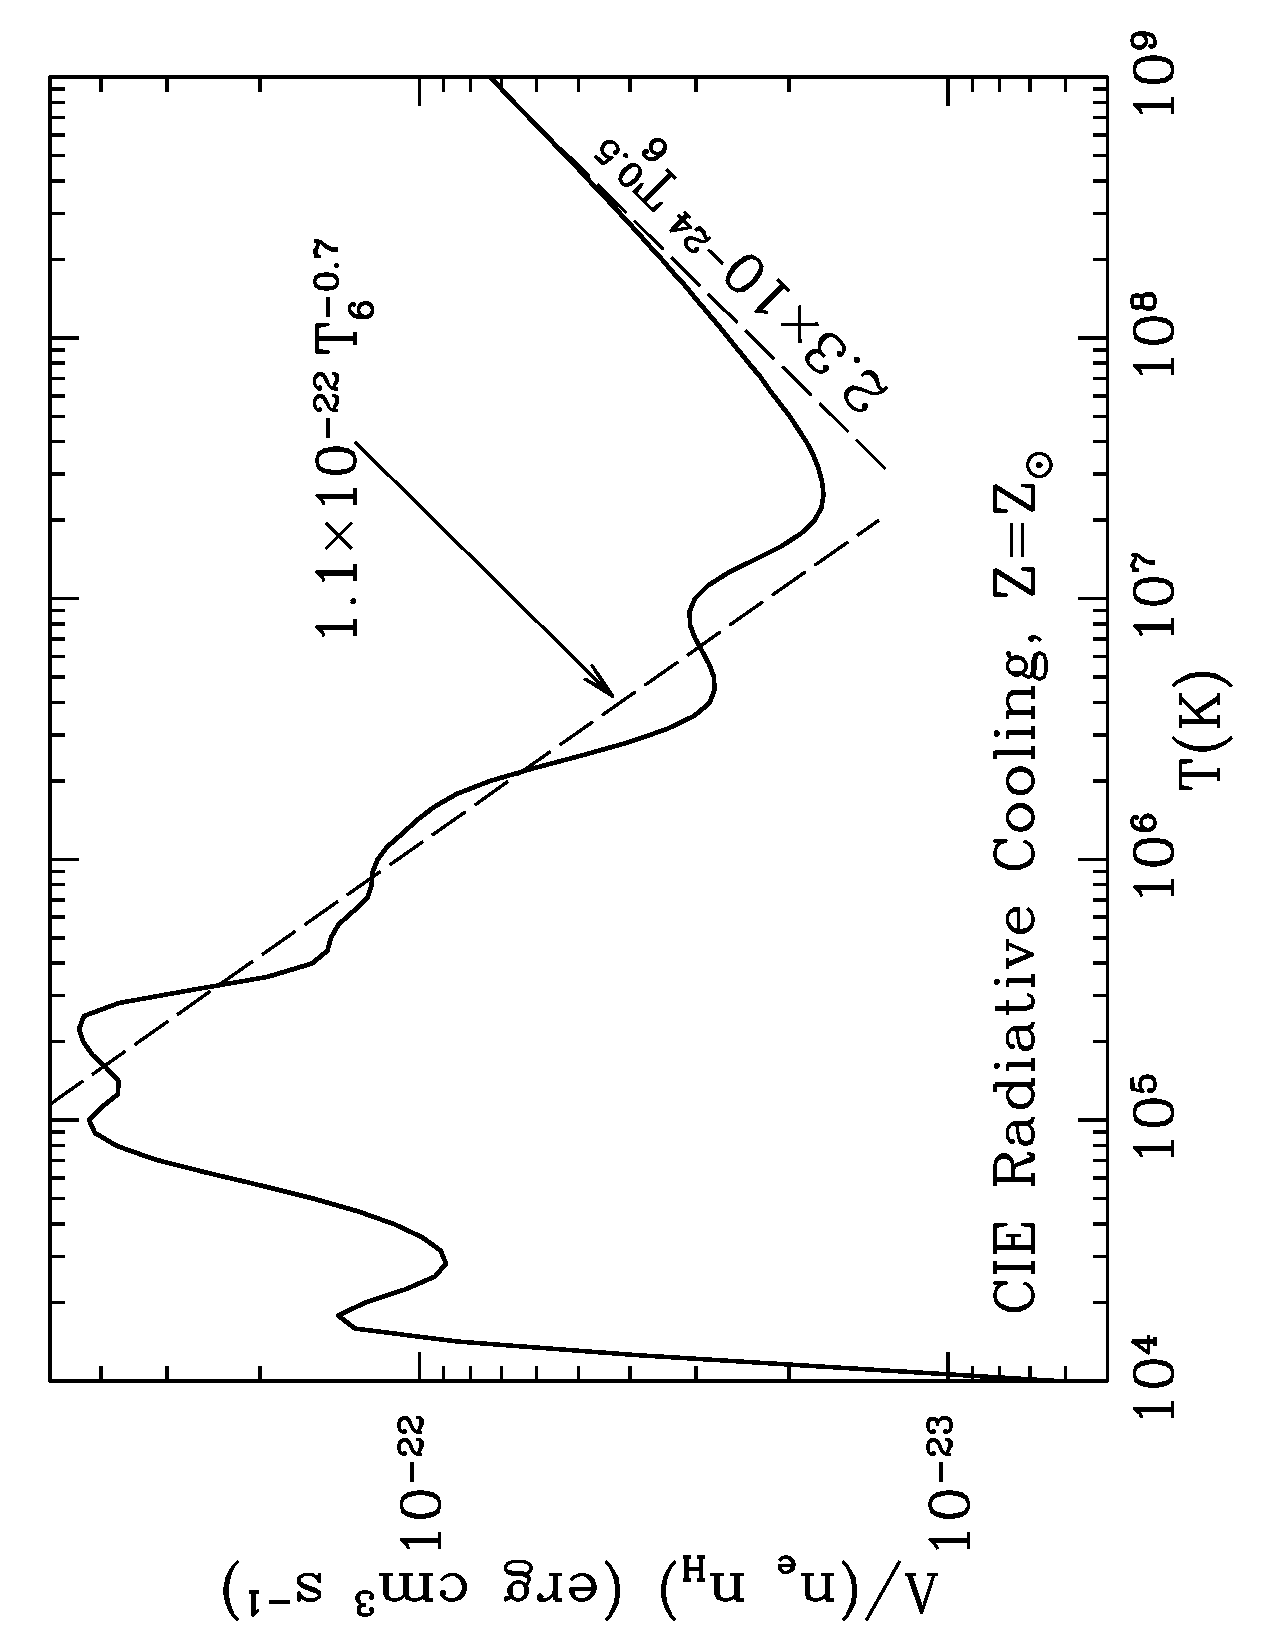
\includegraphics[angle=-90]{ism_figures/Draine-34_1}
\caption{The cooling curve as a function of temperature (Draine Figure 34.1). Note that cooling is inefficient at $T \sim 10^7$ K.}
\end{marginfigure}

The \textbf{hot ionized medium} (HIM) is the dominant phase of the local ISM by volume.

Let's now consider the thermal energy density ($\frac{3}{2}n k T$) changed by a volumetric cooling rate,
\[\frac{d}{dt}\left (\frac{3}{2}n_H kT\right ) = \Lambda,\]
which can be expressed in terms of a \textbf{cooling curve}, $F(T)$:
\begin{equation}
F(T) = \frac{\Lambda}{n_H^2} = \frac{3k}{2n_H}\frac{dT}{dt}.
\end{equation}
This cooling curve is shown in the figure to the right.

How long does it take to cool from $T_0\rightarrow T_0/2$?
\begin{align*}
t &= \frac{3k}{2n_H}\int_{T_0/2}^{T_0}\frac{dT}{F(T)}\\
&\sim \frac{3kT_0}{8n_H}\left [\frac{1}{F(T_0)} + \frac{1}{F(T_0/2)}\right ].
\end{align*} 
In the last step, we've approximated $\int dT/F(T) \sim \Delta T \cdot \ev{1/F(T)}$. These gas cooling timescales are shown in Lecture 21 Equation 8 (which assumes that $x = 0.1$ and $n_H$ in units of cm$^{-3}$. There is a rapid drop in $F(T)$ at $T < 10^4$ K, causing gas to ``hang up'' at $\sim 10^4$ K and not cool efficiently above that.

At this point, we can make a nice big table of phases of the ISM (sorta like we did on 2 October):

\begin{tabular}{c|ccccccccc}
& $n_H$  & $T$ & $nT$ & Fractional volume & Scale height & Surface density \\
& [${\rm cm^{-3}}$] & [K] & [K cm$^{-3}$] & & [pc] & $M_\odot\,\textrm{pc}^{-2}$  \\
\hline
HIM & 0.004 & $\geq 3\e{5}$ & $\geq 1200$ & $\sim 0.5$ & 3000 & 0.3 \\
WIM & $0.3-10^4$ & $10^4$ & $\geq 3000$ & 0.1 & 900 & 1.1 \\
WNM & 0.6 & 5000 & 3000 & 0.4 & $220-400$ & 2.9\\
CNM & 30 & 100 & 3000 & 0.01 & 94 & 2.3\\
GMCs & $10^3-10^6$ & 10-50 & $> 2000$ & $0.0001$ & 75 & 1.0
\end{tabular}


\vspace{2em}

As we can see, the \textit{volume} is dominated by warmer, diffuse phases, whereas the \textit{mass} is dominated by cooler, dense phases. All phases are basically in pressure equilibrium, except the self-gravitating GMCs.

We now introduce the \textbf{three-phase ISM}, which is introduced by McKee \& Ostriker (1977).
At first, the three phases were \textit{clouds} (CNM), the \textit{cloud surfaces} (WNM \& WIM), and \textit{inter-cloud gas} (HIM); they produced this model when contemplating the topology of the ISM when heated by SNe.

We can estimate the volumetric rate of supernova explosions in the Galactic disk to be $S \sim 10^{-13} \,{\rm pc^{-3}\, yr^{-1}}$. The probability that a second supernova will go off within the volume of the a first's remnant is $P_{\rm overlap} = \frac{4\pi}{3}R_{\rm fade}^3 S t_{\rm fade}\sim 0.3$.\sidenote{We know that $t_{\rm fade} \sim 1.7\e{6}$ yr.} It's evident that there will be overlap, and that the topology of the HIM won't be trivial (isolated bubbles). New SNe can rapidly drive pressure through other ionized bubbles, or ``tunnel'' along them.

The McKee \& Ostriker model of the ISM includes:
\begin{enumerate}
\item Three phases of the ISM that are in pressure equilibrium
\item Pressure maintained by supernova remnants, with self-regulated pressure equilibrium
\item Mass equilibrium: cycle of material through the three phases of ISM:
\begin{itemize}
\item some HIM becomes a cool, dense shell swept up at the edge of a SNR
\item shell fragments into cool cloud cores (CNM and eventually GMCs)
\item cores heated and ionized by contact with HIM, producing WNM \& WIM
\item tenous WNM \& WIM material on outer edges of clouds \textit{evaporating} back into HIM
\end{itemize}
\end{enumerate}

Regarding the last point about \textbf{thermal evaporation}, we can calculate the \textit{heat flow} into a cloud via  $K |\nabla T|4\pi r^2 \simeq 4\pi r KT$ (which is in terms of the conductivity $K(T) \simeq 6.1\e{-7}\, (T/\textrm{K})^{-5/2} \, {\rm erg \, s^{-1}\, K^{-1}\, cm^{-1}}$). The energy deposited into the gas flowing away from the cloud causes evaporation at a rate
\begin{equation}
\dot M = \frac{16\pi}{25} \frac{\mu}{k}rK(T),
\end{equation}
where $\mu$ is the average mass of the gas particles.

McKee \& Ostriker predict a spectrum of cloud masses given by $dN \propto R^{-4}\,dR \propto M^{-2}\,dM$, such that small clouds dominate the surface area and evaporation like $d\dot M \propto R\,dN \propto R^{-3}\, dR$. This model does pretty well, except that it underpredicts the mass in the WNM.


\section{Friday, 20 November}
\subsection{Global star formation rates}
Regarding this section title, ``global'' refers to the SFR of entire galaxies. Much of this content comes from Kennicutt \& Evans (2012). What are good SFR estimators?
\begin{enumerate}
\item \textit{Stellar UV continuum emission} (from stars with masses $M_* > 8\, M_\odot$) estimates the SFR averaged over the past $\sim 100$ Myr.\sidenote{This 100 Myr timescale is considered ``instantaneous.''} We have to assume an IMF to convert from massive star formation ($\dot M_{> 8\,M_\odot}$) to total star formation ($\dot M_{> 0.08\,M_\odot}$). However, this will need to be corrected for dust.
\item \textit{Recombination line emission} (usually the Balmer series, sometmies Pa$\alpha$, etc.) is dominated by stars with $M_* \geq 10\, M_\odot$ and lifetimes $\leq 20$ Myr. H$\alpha$ is considered to be the ``gold standard'' (Kennicutt).
\item \textit{Collisional line emission}, e.g., the [\spec{O}{II}] 3727\,\AA{} doublet, can also be a SFR indicator. The [\spec{O}{II}] is a nebular emission line and can be seen at optical wavelengths out to $z = 1.5$.
\item \textit{FIR dust continuum emission} at $40-120\, \upmu$m, or \textit{total IR emission} from $8-1000 \,\upmu$m, which is due to dust heating--mostly from OB stellar light--and traces SFR in highly dust obscured or very actively star-forming galaxies. To a small extent, it also processes general radiation from old stars.
\item \textit{Total inventory of SF}, determined by summing the $L_{\rm UV} + L_{\rm IR}$ gets you the total SFR. Note that upwards of half the UV radiation can be extinguished by dust.\sidenote{BThis isn't always constant, as $L_{\rm IR}/L_{\rm UV} \sim 0.1 - 10^5$, which is a huge range! In very dusty galaxies, using just $L_{\rm IR}$ is reasonable.}
\item \textit{X-ray luminosity} (excluding AGN) is dominated by thermal \textit{bremsstrahlung} high-mass X-ray binaries (HMXBs) from massive stars. We need to correct for low-mass X-ray binaries (LMXBs), which trace stellar mass (but contribute only a bit of $L_{\rm X}$), and also correct for obscuration by atoms such as Fe.
\item \textit{Radio continuum emission}, whereby O stars ($M_* > 10\,M_\odot$) ionize the gas and lead to free-free emission, and also explode in Type II SNe, whose remnants generate synchrotron emission. We also need to exclude AGN in this case.\marginnote{There is a remarkable result linking points 4 and 7 called the \textbf{radio-FIR correlation}. Radio emission at $\nu = 1.4$ GHz and FIR emission are tightly correlated over \textit{five orders of magnitude} of SFR. The FIR emission traces OB stars whereas radio continuum emission traces mostly just O stars, so it's odd to have such a strong correlation.}
\end{enumerate}

\subsection{Global SFR and gas content}
Stars from molecular gas; we often will use the CO luminosity as a proxy for gas mass (or sometimes, HCN as a proxy for dense gas mass), and often use the IR luminosity as a proxy for SFR. We can see that $L_{\rm IR}/L_{\rm CO}' \sim$ SFR/$M_{\rm gas}$, which is the inverse of the gas depletion time, or a \textit{star formation efficiency} (SFE).\sidenote{Note that specific SFR (sSFR) has the same dimensions and is related to SFE, but is not the same thing as SFE.}

\[L_{\rm IR}/L_{\rm CO}' \propto \left (L_{\rm CO}'\right )^x \propto \left (L_{\rm IR}\right )^{\frac{x}{1+x}},\]
where $x \simeq 0.25-0.44$ (Gao \& Solomon 2004a,b). Modulo the brightest IR galaxies (especially those with dust-obscured AGN), this relation should work well. Additionally, HCN $(1-0)$ luminosity correlations more strongly and linearly with $L_{\rm IR}$, with $L_{\rm IR}\propto (L_{\rm HCN}')^{1+x}$, where $x \simeq 0.0-0.05$. This makes sense, because a higher fraction of the densest gas is being turned into stars.

\subsection{The Schmidt law}
Schmidt (1959) found a power-law between SFR and gas density: SFR $\propto \rho^{1.5}$ (where the exponent is based on modern data). But it's very hard to figure out the density of a disk, so we often use 2-D surface densities, called the Schmidt-Kennicutt law (Kennicutt 1998):
\begin{equation}
\frac{\Sigma_{\rm SFR}}{M_\odot \rm\, yr^{-1}\, kpc^{-2}} = (2.5 \pm 0.7)\e{-4} \left (\frac{\Sigma_{\rm gas}}{M_\odot \, \rm pc^{-2}}\right )^{1.4 \pm 0.15}.
\end{equation}

There are competing interpretations for the basis of the Schmidt-Kennicutt law:
\begin{enumerate}
\item The SFR surface density is tied to the free-fall time scale ($t_{\rm ff} \sim 1/ \sqrt{G\rho}$), so that
\[\Sigma_{\rm SFR} \propto \frac{\rho_{\rm gas}}{t_{\rm ff}} \propto \rho_{\rm gas}^{1.5}.\]
A constant scale height is assumed, so that $\rho_{\rm gas} \propto \Sigma_{\rm gas}$ and we recover the Schmidt-Kennicutt law. But this requires some fine tuning since SF doesn't occur through free-fall, and personally I think this is rubbish.
\item If we try to invoke some relation between SFR and orbital timescales by using $\Omega_{\rm dyn} = 2\pi/t_{\rm dyn}$, which is the angular velocity at half-maximum radius of disk. Kennicutt (1998) finds
\[\frac{\Sigma_{\rm SFR}}{M_\odot \rm\, yr^{-1}\, kpc^{-2}} = 0.017 \left (\frac{\Sigma_{\rm gas}}{M_\odot\, \rm pc^{-2}}\right )\left (\frac{\Omega_{\rm dyn}}{\rm yr^{-1}}\right )\]
to be a reasonable fit, requiring a 10\% conversion of gas into stars per orbit. This last point is also rather fine-tuned (across many galaxies).
\item Wong \& Blitz (2002) note that star formation is a two-stage process, in which molecular clouds, and then stars are formed. They trace the power-law index, $n$:
\begin{align}
n &= \frac{d \ln \Sigma_{\rm SFR}}{d\ln \Sigma_{\rm gas}} \nonumber \\
&= \frac{d\ln \Sigma_{\rm SFR}}{d \ln \Sigma_{\Htwo}}\frac{d\ln \Sigma_{\Htwo}}{d\ln \Sigma_{\rm gas}}\nonumber\\
&= n_{\rm mol}\left (1 + \frac{d\ln f_{\rm mol}}{d\ln \Sigma_{\rm gas}}\right ),
\end{align}
where in the last step, $n_{\rm mol}$ is the index of a new Schmidt-like relation between SFR surface density and \textit{molecular} gas surface density, $\Sigma_{\Htwo} = f_{\rm mol} \Sigma_{\rm gas}$ is the fraction of . As a result of the greater total gas surface density, the mid-plane pressure, $P_{\rm midplane}$ is higher but still in hydrostatic equilibrium:
\begin{equation}
P_{\rm midplane} \simeq \frac{\pi}{2}G \Sigma_{\rm gas}\left (\Sigma_{\rm gas} + \frac{\sigma_{\rm gas}}{\sigma_*}\Sigma_*\right )
\end{equation}
where $\sigma_{\rm gas}$, $\sigma_{*}$ are the velocity dispersions of the gas and stars. This relation naturally explains why the SFR$\rightarrow 0$ at $\Sigma_{\rm gas} \leq 5-10 \, M_\odot \rm pc^{-2}$ is purely atomic gas.
\end{enumerate}


\section{Tuesday, 1 December}
\subsection{Spatially resolved star formation}

\noindent Spiral arms of galaxies are \textbf{density waves} in which:
\begin{itemize}
\item[-] gas enters the arm from behind (concave side)
\item[-] molecular clouds are compressed, creating massive molecular associations.
\item[-] pre-existing magnetic fields are compressed, resulting in a local enhancement of synchrotron emission
\item[-] massive star formation occurs (after a time delay for collapse)
\item[-] young stars continue to move towards the front, emerging from their birth clouds on the front side of the arms \marginnote{The phase difference between the optical and UV/radio synchrotron spiral arms can reveal the dynamics.}
\item[-] young stars that are blue but less massive (e.g., A stars) occupy a broader arm and are spread farther ahead
\end{itemize}

\noindent A \textbf{starburst} is a relatively compact region in a galaxy in which:
\begin{itemize}
\item[-] large quantities of gas are available for star formation
\item[-] SFR in the region is $1-100\, M_\odot\,\rm yr^{-1}$
\item[-] SFR surface density $\Sigma_{\rm SFR} \sim 10\, M_\odot\,\rm yr^{-1}\, kpc^{2}$ (distinctive condition of starbursts)\marginnote{Examples can be found in the archetypical dwarf starburst, M82, and archetypical merging galaxy starburst, Arp 220.}
\item[-] the burst timescale is short ($\sim 10^8\, \rm yr$)
\item[-] a large fraction of stars can be formed in \textbf{super star clusters} (SSCs)
\end{itemize}

\subsection{Observational evidence for feedback}

Feedback is the injection of energy and momentum back into the ISM by hot stars, supernovae, and active galactic nuclei. But why is it important? Indirect arguments that feedback ``solves'' some problems:
\begin{itemize}
\item[-] Lower-mass galaxies have lower $Z$ (metallicity) and lower effective yields ($M_Z/M_\star$), because it's easier to blow enriched gas out of the low-mass galaxies via SNe. These feedback mechanisms are called \textbf{galactic winds}.
\item[-] cD\sidenote{A backformation of cD is ``central dominant,'' although it was originally part of the Yerkes galaxy classification scheme.} galaxies at centers of galaxy clusters do not show the expected SFR, given rates at which the intracluster medium (ICM) should be cooling in local instabilities (the ``cooling flow problem''). \textbf{AGN feedback} solves this problem by periodically injecting energy and momentum and shut off star formation.
\item[-] Models of galaxy evolution struggle to make star formation in the most massive galaxies shut off rapidly enough to explain their red colors (the ``quenching problem'').\sidenote{There is actually a low level of star formation in ellipticals too, but whatever.} AGN feedback is also the likely culprit for shutting off star formation.
\end{itemize}

Large-scale galaxy winds are also known as \textbf{superwinds} (see, e.g., the review by Veilleux et al. 2005). Observational evidence for superwinds include:
\begin{enumerate}
\item ionized species (H$\alpha$ reveal edge-brightened features with (bi)conical geometry, suggestive of outflows
\item hot ($T\sim 10^6$ K) X-ray emitting gas, due to free-free emission; also edge-on galaxies show large radio halos
\item outflowing neutral gas--a key line of investigation for winds; locally we can study the Na D doublet at 5890, 5896 \AA{} in absorption to measure outflows\sidenote{We can break the degeneracy between optical depth, $\tau$, and covering factor, the fraction of background source covered by absorbing cloud, but measuring line ratios.}. Dwarf galaxies drive $0.001-1\, M_\odot \,\rm yr^{-1}$, and ULIRGs drive $10-1000\, M_\odot\,\rm yr^{-1}$.
\item outflowing molecular gas and dust
\item existence of a hot halo in Milky Way, which implies a ``Galactic fountain.''\sidenote{This refers to gas being heated and blown out by feedback, cools far away, condenses into neutral clouds that ``rain'' back down onto the MW disk.}
\end{enumerate}

\subsection{Driving mechanisms for galactic winds}
It turns out that there are two possibilities for driving winds: \textbf{energy-driven} vs. \textbf{momentum-driven}. All winds take the path of least resistance, by the way, so they will be launched perpendicular to the disk. Let's consider $\dot M_W$, the rate of mass loss, and $v_\infty$, the terminal velocity of a wind (after the material is far away enough and acceleration ceases). The energy-driven winds would have a constant rate of energy injection, $\dot E \approx \frac{1}{2}\dot M_W v_\infty^2$, and momentum-driven winds require a constant rate of momentum injection, $\dot p \approx \dot M_W v_\infty$.\sidenote{Check out Murray et al. (2005) for more on the theoretical underpinnings and justifications.}

Energy-driven winds are also known as \textit{thermally-driven} or \textit{pressure-driven} (the latter of which might be misleading). A key parameter is the \textit{thermalization efficiency}, $\xi$, which is the fraction of SN energy that heats the ISM. Another useful term (though not used in our crude analysis) is the \textit{mass loading factor}, $\Lambda$, which is the ratio between total mass swept up in a wind and mass released directly by SNe, stars, or AGN.

Suppose we have a SFR of $1\, M_\odot\,\rm yr^{-1}$ causes 1 SN every 100 yr (frequency $\nu_{\rm SN}$), each SN injects $10^{51} \cdot \xi $ erg into the ISM. The net heating rate is then
\begin{equation}
\dot E_{\rm SN} = \xi E_{\rm SN} \nu_{\rm SN} \sim 3\e{40} \left (\frac{\xi}{0.1}\right )\left (\frac{\dot M_\star}{M_\odot\, \rm yr^{-1}}\right ) \textrm{\,erg\, s}^{-1}.
\end{equation}

The net heating rate, after adding in massive stars, is $\dot E_{\rm mech} \sim 2 \times \dot E_{\rm SN}$ (obviously this is silly and fairly inaccurate). Were we to relate the luminosity to SFR by defining efficiency, $\epsilon$:\sidenote{SB stands for ``starburst.''}
\begin{equation}
L_{\rm SB} = \epsilon \dot M_\star c^2 = 6\e{43} \left (\frac{\epsilon}{0.001}\right )\left (\frac{\dot M_\star}{M_\odot\, \rm yr^{-1}}\right )\left (\frac{v_\infty}{300\, \rm km \, s^{-1}}\right )^{-2}.
\end{equation}
A luminous O star releases $\sim 10^{53}$ erg over its lifetime, whereas the SN releases $10^{51}$ erg all at once. So $\dot E_{\rm mech} = 0.01 \xi L_{\rm SB}$, and we solve for the mass loss:
\begin{equation}
\label{eq:energy driven outflow}
\dot M_W \approx \left (\frac{\xi}{0.1}\right )\left (\frac{\epsilon}{0.001}\right )\left (\frac{\dot M_\star}{M_\odot \, \rm yr^{-1}}\right )\left (\frac{v_\infty}{300\, \rm km \, s^{-1}}\right )^{-2} M_\odot \rm\, yr^{-1}.
\end{equation}

To unbind the gas, the energy injected in a dynamical time, $t_{\rm dyn} \sim r/ \sigma$, must exceed the gravitational energy (assuming, in this analysis, an isothermal sphere--$M = 2\sigma^2 r/G$):
\begin{align}
\dot E_{\rm mech}t_{\rm dyn} &\geq \frac{GMM_{\rm gas}}{r} \nonumber \\
&\geq \frac{G\sigma}{r^2}f_{\rm gas} M^2 = \frac{4f_{\rm gas}\sigma^5}{G}\nonumber \\
L_{\rm SB} = \frac{\dot E_{\rm mech}}{0.01 \xi} &\geq 2\e{46}\left (\frac{f_{\rm gas}}{0.1}\right )\left (\frac{\xi}{0.1}\right )^{-1}\left (\frac{\sigma}{200\, \rm km\, s^{-1}}\right )^{5} \textrm{erg\, s}^{-1}.
\end{align}
But... how do you get these winds without \textit{ionizing} everything instantaneously? That becomes the trouble, even if the numbers might work out well. 

Momentum-driven winds allow the gas to somehow be pushed out without the harsh ionization effects. A single SN drives $\sim 10 \, M_\odot$ of material at $\sim 3000\,\rm km\, s^{-1}$. So the rate of momentum injection is 
\[\dot p_{\rm SN} \sim 2\e{33} \left (\frac{\dot M_\star}{M_\odot \rm\, yr^{-1}}\right ) \rm g\, cm\, s^{-2}. \]
Again, we handwave-ly double that to account for winds, $\dot p_{\rm mech} \sim 2 \times \dot p_{\rm SN}$, add radiation pressure with optical depth $\tau$ (and therefore momentum flux $\tau L_{\rm SB}/c$) to find
\begin{equation}
\dot p_{\rm rad} \sim 2\e{33} \left (\frac{\tau}{1}\right ) \left (\frac{\epsilon}{0.001}\right )\left (\frac{\dot M_\star}{M_\odot \,\rm yr^{-1}}\right ) \rm g\, cm\, s^{-2}.
\end{equation}

An order of magnitude estimate suggests that $\dot M_W v_{\infty} \simeq 3\times L_{\rm SB}/c$, so that
\begin{equation}
\dot M_W \approx \left (\frac{\epsilon}{0.001}\right )\left (\frac{\dot M_\star}{M_\odot \, \rm yr^{-1}}\right )\left (\frac{v_\infty}{300\, \rm km \, s^{-1}}\right )^{-1} M_\odot \rm\, yr^{-1}.
\end{equation}
It's similar to the energy-driven case in Equation \eqref{eq:energy driven outflow}, except that there's no dependence on $\xi$, and that now it's proportional to $v_{\infty}^{-1}$.

But obviously, this whole time we should have known that \textit{both} energy \textit{and} momentum are important. We should count both, but since we're lazy, we just want to pick which one dominates.

Gas blowout will occur when radiation pressure + mechanical momentum flux exceeds gravity:
\begin{align*}
\frac{dp}{dt} &= - \frac{GM M_{\rm gas}}{r^2} + \frac{3L_{\rm SB}}{c}\\
&= -\frac{4f_{\rm gas} \sigma^4}{G} + \frac{3L_{\rm SB}}{c},
\end{align*}
and so $\dot p \geq 0$ when 
\begin{equation}
L_{\rm SB}\geq \frac{4f_{\rm gas} c \sigma^4}{3 G} = 10^{46} \left (\frac{f_{\rm gas}}{0.1}\right )\left (\frac{\sigma}{200\,\rm km\, s^{-1}}\right )^{4} \rm erg\, s^{-1}.
\end{equation}

Below $\sigma \simeq 100\cdot (\xi/0.1\, \rm km\, s^{-1} )$, the energy-driven wind threshold is smaller, so that low-mass galaxies lose mass to energy-driven winds. High-mass galaxies would thus be more affected by momentum-driven winds. Intriguing and maybe correct speculations:
\begin{itemize}
\item It'd be useful, but difficult, to test whether winds from massive galaxies are momentum-driven.
\item The Faber-Jackson relation for bulges/ellipticals ($L\propto \sigma^4$) might be explained?
\item The $M_{\rm BH} - \sigma$ relation is $M_{\rm BH}\propto \sigma^4$.
\end{itemize}

\end{document}
